%!TEX TS-program = xelatex
\documentclass[a4paper, 11pt]{article}
%LAYOUT
\usepackage[a4paper]{geometry}
%FONTS
\usepackage{fontspec}
\setmainfont{Brill}

%GLOSSES
\usepackage{glossingtool}
\lingset{aboveglftskip=-0.3ex, everygla=\itshape, belowglpreambleskip=-0.5ex, everyglpreamble=\itshape}
\DeclareAcronym{1}{short=1,long=first~person,short-format=\scshape}
\DeclareAcronym{1+2}{short=1+2,long=first~person~inclusive,short-format=\scshape}
\DeclareAcronym{1+3}{short=1+3,long=first~person~exclusive,short-format=\scshape}
\DeclareAcronym{2}{short=2,long=second~person,short-format=\scshape}
\DeclareAcronym{3}{short=3,long=third~person,short-format=\scshape}
\DeclareAcronym{a}{short=A,long=agent-like~argument~of~canonical~transitive~verb,short-format=\scshape}
\DeclareAcronym{agt}{short=agt,long=agent,short-format=\scshape}
\DeclareAcronym{ana}{short=ana,long=anaphoric,short-format=\scshape}
\DeclareAcronym{attrz}{short=attrz,long=attributivizer,short-format=\scshape}
\DeclareAcronym{caus}{short=caus,long=causative,short-format=\scshape}
\DeclareAcronym{cert}{short=cert,long=certainty,short-format=\scshape}
\DeclareAcronym{com}{short=com,long=comitative,short-format=\scshape}
\DeclareAcronym{cont}{short=cont,long=continuative,short-format=\scshape}
\DeclareAcronym{cor}{short=cor,long=coreference,short-format=\scshape}
\DeclareAcronym{dem}{short=dem,long=demonstrative,short-format=\scshape}
\DeclareAcronym{des}{short=des,long=desiderative,short-format=\scshape}
\DeclareAcronym{detrz}{short=detrz,long=detransitivizer,short-format=\scshape}
\DeclareAcronym{dub}{short=dub,long=dubitative,short-format=\scshape}
\DeclareAcronym{evid}{short=evid,long=evidentiality,short-format=\scshape}
\DeclareAcronym{frust}{short=frust,long=frustrative,short-format=\scshape}
\DeclareAcronym{hsy}{short=hsy,long=hearsay/indirect~evidentiality,short-format=\scshape}
\DeclareAcronym{imm}{short=imm,long=immentiate~past,short-format=\scshape}
\DeclareAcronym{imp}{short=imp,long=imperative,short-format=\scshape}
\DeclareAcronym{inan}{short=inan,long=inanimate,short-format=\scshape}
\DeclareAcronym{inf}{short=inf,long=infinitive,short-format=\scshape}
\DeclareAcronym{intr}{short=intr,long=intermediate~past,short-format=\scshape}
\DeclareAcronym{ints}{short=ints,long=intensifier,short-format=\scshape}
\DeclareAcronym{lk}{short=lk,long=linker,short-format=\scshape}
\DeclareAcronym{loc}{short=loc,long=locative,short-format=\scshape}
\DeclareAcronym{med}{short=med,long=medial,short-format=\scshape}
\DeclareAcronym{neg}{short=neg,long=negation,short-format=\scshape}
\DeclareAcronym{nmlz}{short=nmlz,long=nominalizer,short-format=\scshape}
\DeclareAcronym{npst}{short=npst,long=non-past,short-format=\scshape}
\DeclareAcronym{obl}{short=obl,long=oblique,short-format=\scshape}
\DeclareAcronym{p}{short=p,long=patient-like~argument~of~canonical~transitive~verb,short-format=\scshape}
\DeclareAcronym{pfv}{short=pfv,long=perfective,short-format=\scshape}
\DeclareAcronym{pl}{short=pl,long=plural,short-format=\scshape}
\DeclareAcronym{pro}{short=pro,long=pronoun,short-format=\scshape}
\DeclareAcronym{prs}{short=prs,long=present,short-format=\scshape}
\DeclareAcronym{pst}{short=pst,long=past,short-format=\scshape}
\DeclareAcronym{rec}{short=rec,long=recent~past,short-format=\scshape}
\DeclareAcronym{rem}{short=rem,long=remote~past,short-format=\scshape}
\DeclareAcronym{s}{short=s,long=single~argument~of~canonical~intransitive~verb,short-format=\scshape}
\DeclareAcronym{sa}{short=S\textsubscript{A},long=S~marked~like~A,short-format=\scshape}
\DeclareAcronym{sp}{short=S\textsubscript{P},long=S~marked~like~P,short-format=\scshape}
\DeclareAcronym{sap}{short=sap,long=speech~act~participant,short-format=\scshape}
\DeclareAcronym{sup}{short=sup,long=supine,short-format=\scshape}
\DeclareAcronym{tam}{short=TAM,long=tense-aspect-mood,short-format=\scshape}
\DeclareAcronym{tr}{short=tr,long=transitive,short-format=\scshape}
\DeclareAcronym{uncert}{short=uncert,long=uncertainty,short-format=\scshape}
\DeclareAcronym{inter}{short=inter,long=interrogative,short-format=\scshape}
\DeclareAcronym{int}{short=int,long=intermediate~past,short-format=\scshape}
\DeclareAcronym{all}{short=all,long=allative,short-format=\scshape}
\DeclareAcronym{dat}{short=dat,long=dative,short-format=\scshape}

%FONTS
\usepackage{fontspec}
\setmainfont{Brill}

%HEADERS AND FOOTERS
\usepackage{fancyhdr}
\pagestyle{fancy}
\fancyhead[L,C]{}
\fancyhead[R]{DRAFT (\today)}
\fancyfoot[L]{}
\fancyfoot[C]{\thepage}
\setlength{\headheight}{14.5pt}

%FIRST MENTIONS
\newcommand{\firstmention}[1]{\textsc{#1}}

% LINENUMBERS
%\usepackage{lineno}
\newcommand{\linenumbers}{}
%\documentclass[letterpaper, 12pt]{article}

%LAYOUT
\usepackage[left=2.54cm, right=2.54cm, top=2.54cm, bottom=2.54cm]{geometry}

%SPACING
%\usepackage{setspace}
%\doublespacing

%GLOSSES
\usepackage{glossingtool}
\definelingstyle{IJAL}{labelwidth=2em,labelanchor=numleft, labeloffset=0pt,labelformat=(A),everylabel=\actualexno, textanchor=normal,textoffset=1em,preambleanchor=text, preambleoffset=0pt,avoidnumlabelclash, appendtopexarg={samplelabel=(\actualexno a)}}
\lingset{aboveglftskip=-0.3ex, everygla=\itshape, belowglpreambleskip=-0.5ex, everyglpreamble=\itshape, lingstyle=IJAL}
\DeclareAcronym{1}{short=1,long=first~person,short-format=\scshape}
\DeclareAcronym{1+2}{short=1+2,long=first~person~inclusive,short-format=\scshape}
\DeclareAcronym{1+3}{short=1+3,long=first~person~exclusive,short-format=\scshape}
\DeclareAcronym{2}{short=2,long=second~person,short-format=\scshape}
\DeclareAcronym{3}{short=3,long=third~person,short-format=\scshape}
\DeclareAcronym{a}{short=A,long=agent-like~argument~of~canonical~transitive~verb,short-format=\scshape}
\DeclareAcronym{agt}{short=agt,long=agent,short-format=\scshape}
\DeclareAcronym{ana}{short=ana,long=anaphoric,short-format=\scshape}
\DeclareAcronym{attrz}{short=attrz,long=attributivizer,short-format=\scshape}
\DeclareAcronym{caus}{short=caus,long=causative,short-format=\scshape}
\DeclareAcronym{cert}{short=cert,long=certainty,short-format=\scshape}
\DeclareAcronym{com}{short=com,long=comitative,short-format=\scshape}
\DeclareAcronym{cont}{short=cont,long=continuative,short-format=\scshape}
\DeclareAcronym{cor}{short=cor,long=coreference,short-format=\scshape}
\DeclareAcronym{dem}{short=dem,long=demonstrative,short-format=\scshape}
\DeclareAcronym{des}{short=des,long=desiderative,short-format=\scshape}
\DeclareAcronym{detrz}{short=detrz,long=detransitivizer,short-format=\scshape}
\DeclareAcronym{dub}{short=dub,long=dubitative,short-format=\scshape}
\DeclareAcronym{evid}{short=evid,long=evidentiality,short-format=\scshape}
\DeclareAcronym{frust}{short=frust,long=frustrative,short-format=\scshape}
\DeclareAcronym{hsy}{short=hsy,long=hearsay/indirect~evidentiality,short-format=\scshape}
\DeclareAcronym{imm}{short=imm,long=immentiate~past,short-format=\scshape}
\DeclareAcronym{imp}{short=imp,long=imperative,short-format=\scshape}
\DeclareAcronym{inan}{short=inan,long=inanimate,short-format=\scshape}
\DeclareAcronym{inf}{short=inf,long=infinitive,short-format=\scshape}
\DeclareAcronym{intr}{short=intr,long=intermediate~past,short-format=\scshape}
\DeclareAcronym{ints}{short=ints,long=intensifier,short-format=\scshape}
\DeclareAcronym{lk}{short=lk,long=linker,short-format=\scshape}
\DeclareAcronym{loc}{short=loc,long=locative,short-format=\scshape}
\DeclareAcronym{med}{short=med,long=medial,short-format=\scshape}
\DeclareAcronym{neg}{short=neg,long=negation,short-format=\scshape}
\DeclareAcronym{nmlz}{short=nmlz,long=nominalizer,short-format=\scshape}
\DeclareAcronym{npst}{short=npst,long=non-past,short-format=\scshape}
\DeclareAcronym{obl}{short=obl,long=oblique,short-format=\scshape}
\DeclareAcronym{p}{short=p,long=patient-like~argument~of~canonical~transitive~verb,short-format=\scshape}
\DeclareAcronym{pfv}{short=pfv,long=perfective,short-format=\scshape}
\DeclareAcronym{pl}{short=pl,long=plural,short-format=\scshape}
\DeclareAcronym{pro}{short=pro,long=pronoun,short-format=\scshape}
\DeclareAcronym{prs}{short=prs,long=present,short-format=\scshape}
\DeclareAcronym{pst}{short=pst,long=past,short-format=\scshape}
\DeclareAcronym{rec}{short=rec,long=recent~past,short-format=\scshape}
\DeclareAcronym{rem}{short=rem,long=remote~past,short-format=\scshape}
\DeclareAcronym{s}{short=s,long=single~argument~of~canonical~intransitive~verb,short-format=\scshape}
\DeclareAcronym{sa}{short=S\textsubscript{A},long=S~marked~like~A,short-format=\scshape}
\DeclareAcronym{sp}{short=S\textsubscript{P},long=S~marked~like~P,short-format=\scshape}
\DeclareAcronym{sap}{short=sap,long=speech~act~participant,short-format=\scshape}
\DeclareAcronym{sup}{short=sup,long=supine,short-format=\scshape}
\DeclareAcronym{tam}{short=TAM,long=tense-aspect-mood,short-format=\scshape}
\DeclareAcronym{tr}{short=tr,long=transitive,short-format=\scshape}
\DeclareAcronym{uncert}{short=uncert,long=uncertainty,short-format=\scshape}
\DeclareAcronym{inter}{short=inter,long=interrogative,short-format=\scshape}
\DeclareAcronym{int}{short=int,long=intermediate~past,short-format=\scshape}
\DeclareAcronym{all}{short=all,long=allative,short-format=\scshape}
\DeclareAcronym{dat}{short=dat,long=dative,short-format=\scshape}

%FONTS
\usepackage{fontspec}
\setmainfont{Linux Libertine}
\newfontfamily\objfont{Linux Libertine} %Doulos SIL does not have italics...
\renewcommand{\obj}[1]{\textit{\objfont#1}}
\renewcommand{\rc}[1]{*\textit{\objfont#1}}
\renewcommand{\ort}[1]{$\langle$\objfont#1$\rangle$}

\lingset{everygla=\itshape\objfont, everyglpreamble=\itshape\objfont, everyglb=\objfont}
\usepackage{newunicodechar}
\newunicodechar{∅}{{\objfont∅}}

%HEADERS AND FOOTERS
\usepackage{fancyhdr}
\pagestyle{fancy}
\fancyhead[L,C,R]{}
\renewcommand{\headrulewidth}{0pt}
%\fancyhead[R]{}
%\fancyfoot[L]{}
\fancyfoot[C]{\thepage}
%\setlength{\headheight}{14.5pt}

%SECTION HEADERS
\usepackage{titlesec}
\titleformat{\section}
{\normalfont\fontsize{14}{14}\bfseries}{\thesection.}{1ex}{}

\titleformat{\subsection}
{\normalfont\fontsize{12}{12}\bfseries}{\thesubsection.}{1ex}{}


%FIRST MENTIONS
\newcommand{\firstmention}[1]{\textit{#1}}

%TITLE AND ABSTRACT
\date{}
\usepackage{etoolbox}
\AtBeginEnvironment{abstract}{\itshape}

\usepackage{placeins}

%FLOATS AND FOOTNOTES
\usepackage[bottom]{footmisc}

% LINENUMBERS
%\usepackage{lineno}
\newcommand{\linenumbers}{}
%\documentclass[a4paper, 11pt, twoside]{article}

%LAYOUT
\usepackage[left=2.4cm,right=2.4cm, top=2.5cm, bottom=2.4cm]{geometry}

%FONTS
\usepackage{fontspec}
\setmainfont{Linux Libertine}

%GLOSSES
\usepackage{glossingtool}
\lingset{aboveglftskip=-0.3ex, everygla=\itshape, belowglpreambleskip=-0.5ex, everyglpreamble=\itshape}
\DeclareAcronym{1}{short=1,long=first~person,short-format=\scshape}
\DeclareAcronym{1+2}{short=1+2,long=first~person~inclusive,short-format=\scshape}
\DeclareAcronym{1+3}{short=1+3,long=first~person~exclusive,short-format=\scshape}
\DeclareAcronym{2}{short=2,long=second~person,short-format=\scshape}
\DeclareAcronym{3}{short=3,long=third~person,short-format=\scshape}
\DeclareAcronym{a}{short=A,long=agent-like~argument~of~canonical~transitive~verb,short-format=\scshape}
\DeclareAcronym{agt}{short=agt,long=agent,short-format=\scshape}
\DeclareAcronym{ana}{short=ana,long=anaphoric,short-format=\scshape}
\DeclareAcronym{attrz}{short=attrz,long=attributivizer,short-format=\scshape}
\DeclareAcronym{caus}{short=caus,long=causative,short-format=\scshape}
\DeclareAcronym{cert}{short=cert,long=certainty,short-format=\scshape}
\DeclareAcronym{com}{short=com,long=comitative,short-format=\scshape}
\DeclareAcronym{cont}{short=cont,long=continuative,short-format=\scshape}
\DeclareAcronym{cor}{short=cor,long=coreference,short-format=\scshape}
\DeclareAcronym{dem}{short=dem,long=demonstrative,short-format=\scshape}
\DeclareAcronym{des}{short=des,long=desiderative,short-format=\scshape}
\DeclareAcronym{detrz}{short=detrz,long=detransitivizer,short-format=\scshape}
\DeclareAcronym{dub}{short=dub,long=dubitative,short-format=\scshape}
\DeclareAcronym{evid}{short=evid,long=evidentiality,short-format=\scshape}
\DeclareAcronym{frust}{short=frust,long=frustrative,short-format=\scshape}
\DeclareAcronym{hsy}{short=hsy,long=hearsay/indirect~evidentiality,short-format=\scshape}
\DeclareAcronym{imm}{short=imm,long=immentiate~past,short-format=\scshape}
\DeclareAcronym{imp}{short=imp,long=imperative,short-format=\scshape}
\DeclareAcronym{inan}{short=inan,long=inanimate,short-format=\scshape}
\DeclareAcronym{inf}{short=inf,long=infinitive,short-format=\scshape}
\DeclareAcronym{intr}{short=intr,long=intermediate~past,short-format=\scshape}
\DeclareAcronym{ints}{short=ints,long=intensifier,short-format=\scshape}
\DeclareAcronym{lk}{short=lk,long=linker,short-format=\scshape}
\DeclareAcronym{loc}{short=loc,long=locative,short-format=\scshape}
\DeclareAcronym{med}{short=med,long=medial,short-format=\scshape}
\DeclareAcronym{neg}{short=neg,long=negation,short-format=\scshape}
\DeclareAcronym{nmlz}{short=nmlz,long=nominalizer,short-format=\scshape}
\DeclareAcronym{npst}{short=npst,long=non-past,short-format=\scshape}
\DeclareAcronym{obl}{short=obl,long=oblique,short-format=\scshape}
\DeclareAcronym{p}{short=p,long=patient-like~argument~of~canonical~transitive~verb,short-format=\scshape}
\DeclareAcronym{pfv}{short=pfv,long=perfective,short-format=\scshape}
\DeclareAcronym{pl}{short=pl,long=plural,short-format=\scshape}
\DeclareAcronym{pro}{short=pro,long=pronoun,short-format=\scshape}
\DeclareAcronym{prs}{short=prs,long=present,short-format=\scshape}
\DeclareAcronym{pst}{short=pst,long=past,short-format=\scshape}
\DeclareAcronym{rec}{short=rec,long=recent~past,short-format=\scshape}
\DeclareAcronym{rem}{short=rem,long=remote~past,short-format=\scshape}
\DeclareAcronym{s}{short=s,long=single~argument~of~canonical~intransitive~verb,short-format=\scshape}
\DeclareAcronym{sa}{short=S\textsubscript{A},long=S~marked~like~A,short-format=\scshape}
\DeclareAcronym{sp}{short=S\textsubscript{P},long=S~marked~like~P,short-format=\scshape}
\DeclareAcronym{sap}{short=sap,long=speech~act~participant,short-format=\scshape}
\DeclareAcronym{sup}{short=sup,long=supine,short-format=\scshape}
\DeclareAcronym{tam}{short=TAM,long=tense-aspect-mood,short-format=\scshape}
\DeclareAcronym{tr}{short=tr,long=transitive,short-format=\scshape}
\DeclareAcronym{uncert}{short=uncert,long=uncertainty,short-format=\scshape}
\DeclareAcronym{inter}{short=inter,long=interrogative,short-format=\scshape}
\DeclareAcronym{int}{short=int,long=intermediate~past,short-format=\scshape}
\DeclareAcronym{all}{short=all,long=allative,short-format=\scshape}
\DeclareAcronym{dat}{short=dat,long=dative,short-format=\scshape}

%FIRST MENTIONS
\newcommand{\firstmention}[1]{\textsc{#1}}

%HEADERS AND FOOTERS
\usepackage{fancyhdr}
\pagestyle{fancy}
\lhead[]{\thepage}
\chead[Conservative first person forms in Cariban]{Cadernos de Etnolingüística}
\rhead[\thepage]{}
\setlength{\headheight}{15pt}

\lfoot{}
\cfoot{}
\rfoot{}

%LINE NUMBERS
\usepackage{lineno}
%\newcommand{\linenumbers}{}

%SPACING
%\usepackage{setspace}
%\onehalfspacing

%FLOATS AND FOOTNOTES
\usepackage[bottom]{footmisc}

\documentclass[a4paper, 11pt]{article}
\usepackage[toc]{appendix}
%FONTS
\usepackage{fontspec}
\setmainfont{Brill}

%LAYOUT
\usepackage[a4paper]{geometry}
%
%\usepackage{setspace}
%\onehalfspacing

%\usepackage{titling}
%\setlength{\droptitle}{-3cm}

\renewcommand{\abstractname}{\vspace{-1.5\baselineskip}}

%CAPTIONS
%\usepackage{caption}
\usepackage{threeparttable}
\usepackage{subcaption}

%TABLES
\usepackage{booktabs}
\providecommand{\mytoprule}{\toprule}
\providecommand{\mymidrule}{\midrule}
\providecommand{\mybottomrule}{\bottomrule}

%GLOSSES
\usepackage{glossingtool}
\lingset{aboveglftskip=-0.3ex, everygla=\itshape, belowglpreambleskip=-0.5ex, everyglpreamble=\itshape}
\DeclareAcronym{1}{short=1,long=first~person,short-format=\scshape}
\DeclareAcronym{1+2}{short=1+2,long=first~person~inclusive,short-format=\scshape}
\DeclareAcronym{1+3}{short=1+3,long=first~person~exclusive,short-format=\scshape}
\DeclareAcronym{2}{short=2,long=second~person,short-format=\scshape}
\DeclareAcronym{3}{short=3,long=third~person,short-format=\scshape}
\DeclareAcronym{a}{short=A,long=agent-like~argument~of~canonical~transitive~verb,short-format=\scshape}
\DeclareAcronym{agt}{short=agt,long=agent,short-format=\scshape}
\DeclareAcronym{ana}{short=ana,long=anaphoric,short-format=\scshape}
\DeclareAcronym{attrz}{short=attrz,long=attributivizer,short-format=\scshape}
\DeclareAcronym{caus}{short=caus,long=causative,short-format=\scshape}
\DeclareAcronym{cert}{short=cert,long=certainty,short-format=\scshape}
\DeclareAcronym{com}{short=com,long=comitative,short-format=\scshape}
\DeclareAcronym{cont}{short=cont,long=continuative,short-format=\scshape}
\DeclareAcronym{cor}{short=cor,long=coreference,short-format=\scshape}
\DeclareAcronym{dem}{short=dem,long=demonstrative,short-format=\scshape}
\DeclareAcronym{des}{short=des,long=desiderative,short-format=\scshape}
\DeclareAcronym{detrz}{short=detrz,long=detransitivizer,short-format=\scshape}
\DeclareAcronym{dub}{short=dub,long=dubitative,short-format=\scshape}
\DeclareAcronym{evid}{short=evid,long=evidentiality,short-format=\scshape}
\DeclareAcronym{frust}{short=frust,long=frustrative,short-format=\scshape}
\DeclareAcronym{hsy}{short=hsy,long=hearsay/indirect~evidentiality,short-format=\scshape}
\DeclareAcronym{imm}{short=imm,long=immentiate~past,short-format=\scshape}
\DeclareAcronym{imp}{short=imp,long=imperative,short-format=\scshape}
\DeclareAcronym{inan}{short=inan,long=inanimate,short-format=\scshape}
\DeclareAcronym{inf}{short=inf,long=infinitive,short-format=\scshape}
\DeclareAcronym{intr}{short=intr,long=intermediate~past,short-format=\scshape}
\DeclareAcronym{ints}{short=ints,long=intensifier,short-format=\scshape}
\DeclareAcronym{lk}{short=lk,long=linker,short-format=\scshape}
\DeclareAcronym{loc}{short=loc,long=locative,short-format=\scshape}
\DeclareAcronym{med}{short=med,long=medial,short-format=\scshape}
\DeclareAcronym{neg}{short=neg,long=negation,short-format=\scshape}
\DeclareAcronym{nmlz}{short=nmlz,long=nominalizer,short-format=\scshape}
\DeclareAcronym{npst}{short=npst,long=non-past,short-format=\scshape}
\DeclareAcronym{obl}{short=obl,long=oblique,short-format=\scshape}
\DeclareAcronym{p}{short=p,long=patient-like~argument~of~canonical~transitive~verb,short-format=\scshape}
\DeclareAcronym{pfv}{short=pfv,long=perfective,short-format=\scshape}
\DeclareAcronym{pl}{short=pl,long=plural,short-format=\scshape}
\DeclareAcronym{pro}{short=pro,long=pronoun,short-format=\scshape}
\DeclareAcronym{prs}{short=prs,long=present,short-format=\scshape}
\DeclareAcronym{pst}{short=pst,long=past,short-format=\scshape}
\DeclareAcronym{rec}{short=rec,long=recent~past,short-format=\scshape}
\DeclareAcronym{rem}{short=rem,long=remote~past,short-format=\scshape}
\DeclareAcronym{s}{short=s,long=single~argument~of~canonical~intransitive~verb,short-format=\scshape}
\DeclareAcronym{sa}{short=S\textsubscript{A},long=S~marked~like~A,short-format=\scshape}
\DeclareAcronym{sp}{short=S\textsubscript{P},long=S~marked~like~P,short-format=\scshape}
\DeclareAcronym{sap}{short=sap,long=speech~act~participant,short-format=\scshape}
\DeclareAcronym{sup}{short=sup,long=supine,short-format=\scshape}
\DeclareAcronym{tam}{short=TAM,long=tense-aspect-mood,short-format=\scshape}
\DeclareAcronym{tr}{short=tr,long=transitive,short-format=\scshape}
\DeclareAcronym{uncert}{short=uncert,long=uncertainty,short-format=\scshape}
\DeclareAcronym{inter}{short=inter,long=interrogative,short-format=\scshape}
\DeclareAcronym{int}{short=int,long=intermediate~past,short-format=\scshape}
\DeclareAcronym{all}{short=all,long=allative,short-format=\scshape}
\DeclareAcronym{dat}{short=dat,long=dative,short-format=\scshape}

%CUSTOM COMMANDS
\usepackage{xspace}
\providecommand{\wbakairi}{Western Bakairi\xspace}
\providecommand{\ebakairi}{Eastern Bakairi\xspace}
\providecommand{\ingariko}{Ingarikó\xspace}
\providecommand{\akawaio}{Akawaio\xspace}
\providecommand{\patamona}{Patamona\xspace}
\providecommand{\yukpa}{Yukpa\xspace}
\providecommand{\japreria}{Japreria\xspace}
\providecommand{\carijo}{Karijona\xspace}
\providecommand{\mapoyo}{Mapoyo\xspace}
\providecommand{\yawarana}{Yawarana\xspace}
\providecommand{\panare}{Panare\xspace}
\providecommand{\maqui}{Ye'kwana\xspace}
\providecommand{\pemon}{Pemón\xspace}
\providecommand{\kapon}{Kapong\xspace}
\providecommand{\waimiri}{Waimiri-Atroari\xspace}
\providecommand{\macushi}{Macushi\xspace}
\providecommand{\waiwai}{Waiwai\xspace}
\providecommand{\hixka}{Hixkaryána\xspace}
\providecommand{\kaxui}{Werikyana\xspace}
\providecommand{\trio}{Tiriyó\xspace}
\providecommand{\akuriyo}{Akuriyó\xspace}
\providecommand{\apalai}{Apalaí\xspace}
\providecommand{\wayana}{Wayana\xspace}
\providecommand{\ikpeng}{Ikpeng\xspace}
\providecommand{\arara}{Arara\xspace}
\providecommand{\kalina}{Kari'ña\xspace}
\providecommand{\uxc}{Upper Xingu Carib\xspace}
\providecommand{\bakairi}{Bakairi\xspace}
\providecommand{\PC}{Proto-Cariban\xspace}
\providecommand{\PPar}{Proto-Parukotoan\xspace}
\providecommand{\PWai}{Proto-Waiwaian\xspace}
\providecommand{\PPek}{Proto-Pekodian\xspace}
\providecommand{\PXin}{Proto-Xinguan\xspace}
\providecommand{\PPP}{Proto-Pemong-Panare\xspace}
\providecommand{\PTar}{Proto-Taranoan\xspace}
\providecommand{\PTir}{Proto-Tiriyoan\xspace}
\newcommand{\notn}{\obj{i-}/Ø/\obj{t(ɨ)-}\xspace}
\newcommand{\yesn}{\obj{n(i)-}/\obj{n(ɨ)-}\xspace}
\newcommand{\setone}{Set I\xspace}
\newcommand{\settwo}{Set II\xspace}
\providecommand{\goodtilde}{\char`~\xspace}
\newcommand{\perscomm}[1]{#1 (p.c.)}
\newcommand{\perscommpar}[1]{(#1, p.c.)}

%TREES
\usepackage{tikz-qtree}

%DRAFT MODE
%\usepackage{draftwatermark}
%\SetWatermarkLightness{0.95}

%\usepackage{lineno}
\newcommand{\linenumbers}{}

%STUBBORN BROKEN SUFFIXES IN RUNNING TEXT
%\usepackage[shortcuts]{extdash}

%HYPHENATION
\hyphenation{Wa-ya-na mar-ker Ti-ri-yó Des-mond An-tro-po-ló-gi-ca}

%BIBLIOGRAPHY
%For diachronica
%\usepackage[backend=biber,
%            bibstyle=biblatex-sp-unified,
%            citestyle=sp-authoryear-comp,
%            maxcitenames=2,
%            mincitenames=1,
%            maxbibnames=99]{biblatex}
%For others
\input{iswbibConfiguration.tex}
\addbibresource{cariban_references.bib}
\addbibresource{non_cariban_references.bib}
\addbibresource{irregular_references.bib}

\newcommand{\glossfootnote}{\footnote{Glossing abbreviations: \glossingAbbrevsComma.}}
\newcommand{\glosssection}{}

%\input{stuff/diachronica.tex}

\usepackage[edges]{forest}

\usepackage{amsfonts}

\usepackage{fancyhdr}
\pagestyle{fancy}
 \fancyhead[L,C]{}
 \fancyhead[R]{DRAFT (\today)}
 \fancyfoot[L]{}
 \fancyfoot[C]{\thepage}
  \setlength{\headheight}{14.5pt}
%CROSSREFS
\usepackage{hyperref}
\usepackage[capitalise,noabbrev]{cleveref}
\newcommand{\pcref}[1]{(\cref{#1})}

\newlist{inlinelist}{enumerate*}{1}
\setlist[inlinelist]{label={\alph*)}, itemjoin={{; }}, itemjoin*={{; and }}}

\newlist{legendlist}{itemize*}{1}
\setlist[legendlist]{itemjoin={{; }}}

\newcommand{\emp}[1]{\textbf{#1}}
\newcommand{\subs}[1]{\textsubscript{#1}}

%to have nice right-hand sources in quotes
\def\signed #1{{\leavevmode\unskip\nobreak\hfil\penalty50\hskip2em
  \hbox{}\nobreak\hfil#1%
  \parfillskip=0pt \finalhyphendemerits=0 \endgraf}}

\newsavebox\mybox
\newenvironment{quotebox}[1]
  {\savebox\mybox{#1}\begin{quotation}}
  {\signed{\usebox\mybox}\end{quotation}}

\newcommand{\detrz}{\rc{əte}\slash{}\obj{e-}}
\usepackage{phonrule}
\usepackage{amsthm,etoolbox,xcolor}

\captionsetup{compatibility=false}

%\usepackage[section]{placeins}
%\let\Oldsection\section
%\renewcommand{\section}{\FloatBarrier\Oldsection}
%
%\let\Oldsubsection\subsection
%\renewcommand{\subsection}{\FloatBarrier\Oldsubsection}
%
%\let\Oldsubsubsection\subsubsection
%\renewcommand{\subsubsection}{\FloatBarrier\Oldsubsubsection}


%\usepackage[nofiglist, notablist]{endfloat}
%
%\AtBeginDocument{%                                                     
%	\DeclareDelayedFloatFlavor{subtable}{table}
%	\DeclareDelayedFloatFlavor{subfigure}{figure}
%}




\newcommand{\pcone}{\\\small\begin{tabular}{@{}rllll@{}}
& \gl{a} & \gl{s_a_} & \gl{s_p_} & \gl{p}\\
\gl{1} & \rc{t(i)-} & \rc{w-} & \rc{u(j)-} & \rc{u(j)-}\\
\gl{2} & \rc{m(i)-} & \rc{m-} & \rc{ə(j)-} & \rc{ə(j)-}\\
\gl{1+2} & \rc{kɨt(i)-} & \rc{kɨt-} & \rc{k-} & \rc{k-}\\
\end{tabular}}

\newcommand{\ppone}{\\\small\begin{tabular}{@{}rllll@{}}
& \gl{a} & \gl{s_a_} & \gl{s_p_} & \gl{p}\\
\gl{1} & \emp{\rc{w-}} & \rc{w-} & \emp{\rc{k-}}, *Ø/\obj{j-} & *Ø/\obj{j-}\\
\gl{2} & \rc{m-} & \rc{m-} & \rc{o(j)-} & \rc{o(j)-}\\
\gl{1+2} & \rc{kɨt-} & \rc{kɨt-} & \rc{k-}, \emp{\rc{kɨt-}} & \rc{k-}\\
\end{tabular}}

\newcommand{\kaxone}{\\\small\begin{tabular}{@{}rllll@{}}
& \gl{a} & \gl{s_a_} & \gl{s_p_} & \gl{p}\\
\gl{1} & \obj{w-} & \obj{w-} & \obj{k-}, Ø/\obj{j-} & Ø/\obj{j-}\\
\gl{2} & \obj{m-} & \obj{m-} & \obj{o-} & \obj{o-}\\
\gl{1+2} & \obj{kɨt-} & \obj{kɨt-} & \obj{k-}, \obj{kɨt-} & \obj{k-}\\
\end{tabular}}

\newcommand{\pwone}{\\\small\begin{tabular}{@{}rllll@{}}
& \gl{a} & \gl{s_a_} & \gl{s_p_} & \gl{p}\\
\gl{1} & \rc{w-} & \emp{\rc{k-}} & \rc{k-} & \emp{\rc{owɨ(ro) j-}}\\
\gl{2} & \rc{m-} & \rc{m-} & \rc{o(j)-} & \rc{o(j)-}\\
\gl{1+2} & \rc{tɨt-} & \rc{tɨt-} & \rc{tɨt-} & \rc{k-}\\
\end{tabular}}

\newcommand{\hixone}{\\\small\begin{tabular}{@{}rllll@{}}
& \gl{a} & \gl{s_a_} & \gl{s_p_} & \gl{p}\\
\gl{1} & \obj{w-}/\obj{ɨ-} & \obj{k-} & \obj{k-} & \obj{r(o)-}\\
\gl{2} & \obj{m-} & \obj{m-} & \obj{o(j)-} & \obj{o(j)-}\\
\gl{1+2} & \obj{t-} & \obj{t-} & \obj{t-} & \obj{k-}\\
\end{tabular}}

\newcommand{\waione}{\\\small\begin{tabular}{@{}rllll@{}}
& \gl{a} & \gl{s_a_} & \gl{s_p_} & \gl{p}\\
\gl{1} & \obj{w-} & \obj{k-} & \obj{k-} & \obj{o(j)-}\\
\gl{2} & \obj{m-} & \obj{m-} & \emp{\obj{m-}} & \obj{a(w)-}\\
\gl{1+2} & \obj{t(ɨt)-} & \obj{t(ɨt)-} & \obj{t(ɨt)-} & \obj{k-}\\
\end{tabular}}

\title{A comparative account of intransitive verbs with conservative first person forms in Cariban}
%\author{}
%\date{}

\begin{document}
%%\begin{center}\Large
%\makeatletter
%\@title
%\makeatother
%\end{center}
%\thispagestyle{empty}
%\pagestyle{empty}
%
%\begin{abstract}
%	\noindent\input{abstract.txt}
%\end{abstract}
%
%%\newpage
%\FloatBarrier
%%\tableofcontents
%%\newpage
%%\listoffigures
%%\listoftables
%%
%%\newpage
%\pagestyle{fancy}
%
%\linenumbers
%
%\setcounter{page}{1}
%\pagenumbering{arabic}
\maketitle	
\thispagestyle{empty}
\pagestyle{empty}

\begin{abstract}
	\input{abstract.txt}
\end{abstract}

\newpage
\tableofcontents
\newpage
\listoffigures
\listoftables

\newpage
\pagestyle{fancy}

\linenumbers

\setcounter{page}{1}
\pagenumbering{arabic}
%%\begin{center}\Large
%	\makeatletter
%	\@title
%	\makeatother
%\end{center}
%\thispagestyle{empty}
%
%\begin{abstract}
%	\begin{center}
%	\bfseries Abstract
%	\end{center}
%	\input{abstract.txt}
%\end{abstract}
%\vspace{0.2cm}
%\noindent Keywords: \input{keywords.txt}
%
%%\newpage
%%\tableofcontents
%%\newpage
%%\listoffigures
%%\listoftables
%%
%%\newpage
%\pagestyle{fancy}
%
%\linenumbers
%
%\setcounter{page}{1}
%\pagenumbering{arabic}
%
%\FloatBarrier

\section{Introduction}
\label{sec:intro}
The Cariban language family is one of the largest of South America, with between 60'000 and 100'000 speakers unevenly distributed between 22 to 25 extant languages \parencite[441]{gildea2012classification}.
The family is concentrated in Venezuela, the Guianas and Northern Brazil, with two Western and four Southern outliers.
\cref{fig:phylomap} shows the geographical distribution and genealogical affiliation of the extant Cariban languages.
%Cariban languages feature relatively rich verbal morphology, both pre- and suffixes, inflecting for person, number, tense, aspect, and evidentiality, combined with a range of valency-modifying affixes.
%Many also have a split-\gl{s} system, which can be reconstructed to \PC \pcref{sec:split}.
For linguistic overviews of and  comparative work on the family, readers are referred to \textcites{gildea1998}{derbyshire1999carib}{meira2002first}{meira2005southern}{meira2006cariban}{gildea2007greenberg}{meira2010origin}{gildea2010story}{gildea2012classification}{matter2021cariban}{gildea2019overview}.

\begin{figure}
	\centering
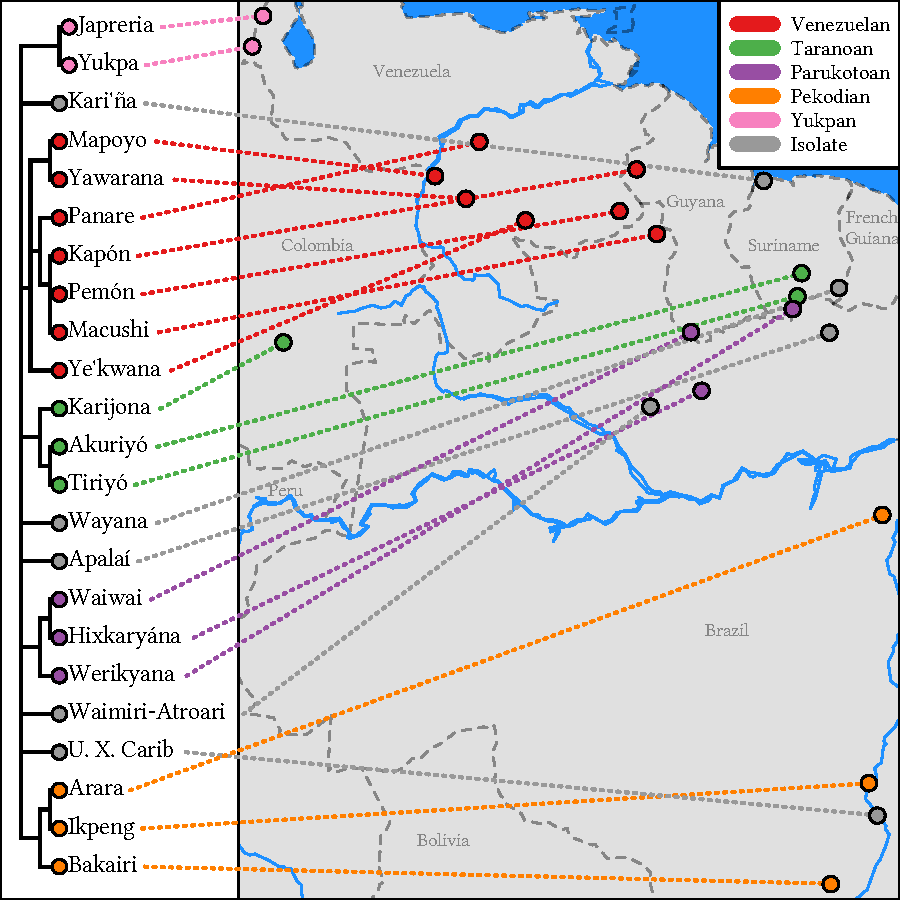
\includegraphics{floats/genealogical_map}
	\caption{The Cariban language family}
	\label{fig:phylomap}
\end{figure}

\begin{table}[htbp]
\centering
\caption[Some \hixka verbs]{Some \hixka verbs \parencites[150, 510, 511, 513, 520]{howard2001wrought}[197, 198]{hixkaryanaderby1985}}
\label{tab:hixintro}
\begin{tabular}[t]{@{}llllll@{}}
\mytoprule
{} &     \qu{to fall} &  \qu{to be afraid} &          \qu{to walk} & \qu{to cut self} &    \qu{to be} \\
\mymidrule
\gl{1}   &  \obj{k-ehurka-} &  \obj{k-oserʲehɨ-} &  \obj{k-atarʲeknohɨ-} &   \obj{k-atama-} &  \obj{w-eʃe-} \\
\gl{2}   &  \obj{m-ehurka-} &  \obj{m-oserʲehɨ-} &  \obj{m-atarʲeknohɨ-} &   \obj{m-atama-} &  \obj{m-eʃe-} \\
\gl{1+2} &  \obj{t-ehurka-} &  \obj{t-oserʲehɨ-} &  \obj{t-atarʲeknohɨ-} &   \obj{t-atama-} &  \obj{t-eʃe-} \\
\gl{3}   &  \obj{ɲ-ehurka-} &  \obj{n-oserʲehɨ-} &  \obj{n-atarʲeknohɨ-} &   \obj{n-atama-} &  \obj{n-eʃe-} \\
\mybottomrule
\end{tabular}
\end{table}
\begin{table}
\centering
\caption[Some \trio verbs]{Some \trio verbs \parencites[292, 294]{triomeira1999}[274]{triocarlin2004}}
\label{tab:triintro}
\begin{tabular}[t]{@{}llllll@{}}
\mytoprule
{} &      \qu{to sleep} & \qu{to see self} & \qu{to bathe (\gl{intr})} &     \qu{to yawn} &     \qu{to go} \\
\midrule
\gl{1}   &    \obj{t-əənɨkɨ-} &    \obj{t-əene-} &              \obj{s-epɨ-} &  \obj{s-entapo-} &  \obj{wɨ-tən-} \\
\gl{2}   &    \obj{m-əənɨkɨ-} &    \obj{m-əene-} &              \obj{m-epɨ-} &  \obj{m-entapo-} &  \obj{mɨ-tən-} \\
\gl{1+2} &  \obj{kɨt-əənɨkɨ-} &    \obj{k-əene-} &             \obj{ke-epɨ-} &  \obj{k-entapo-} &  \obj{kɨ-tən-} \\
\gl{3}   &    \obj{n-əənɨkɨ-} &    \obj{n-əene-} &              \obj{n-epɨ-} &  \obj{n-entapo-} &  \obj{nɨ-tən-} \\
\bottomrule
\end{tabular}
\end{table}

In some Cariban languages, a small group of verbs show a divergent first person inflection pattern, a topic which has not received much attention in the literature.
This is illustrated with person paradigms of four \hixka verbs in \cref{tab:hixintro},\footnote{The presence of a \gl{1+2} person value implies that of a \gl{1+3} value.
This is usually expressed with a free pronoun combined with third person morphology in Cariban languages, so it is not represented as a distinct value in the paradigms shown here.
In \cref{tab:hixintro} and other paradigm tables, any TAM suffixes found in the original forms found in the literature are omitted, since a) the focus lies on the prefixes and stems, and b) full paradigms containing the same TAM suffix are rarely found.
Further, standard IPA symbols are used in the transcription of Cariban languages, with the exception of coronal rhotics, which are simply represented with \ort{r}, rather than \ort{ɽ} for \wayana or \ort{ɾ̠} for \maqui etc.
In languages with strong morphophonological processes and/or subphonemic orthography the original transcription is shown in an additional surface line when presented in interlinearized examples.
\textcite{gildea2018reconstructing} is followed in using \ort{ə} for the proto-vowel reconstructed by \textcite{meira2005southern}, although it was likely more back \parencite{gildea2010story}.
Glossing abbreviations: } %\glossingAbbrevsComma.
all members of the \gl{s_a_} inflectional class.
In this language, the verb \qu{to be} diverges from other \gl{s_a_} verbs like \qu{to fall} by having a first person marker \obj{w-}, rather than \obj{k-}.
A similar pattern exists in \trio, where the verb \qu{to go} has a first-person prefix \obj{wɨ-} while other \gl{s_a_} verbs have a prefix with phonologically conditioned allomorphs \envr{\obj{t-}}{\obj{ə}} and \envr{\obj{s-}}{\obj{e}} \pcref{tab:triintro}.
In both languages, the first person prefix of the verbs on the left is representative for the vast majority of \gl{s_a_} verbs.
%In both languages, there are only a few other verbs inflected identically to the divergent ones on the right; for example, the first-person form of \trio \qu{to be} is \obj{w-ei-} \parencites[339]{triomeira1999}.

Such divergent verbs have been identified for \hixka \parencite[188]{hixkaryanaderby1985}, \waiwai \parencite[90]{gildea1998}, the three Taranoan languages \parencite[112--115]{meira1998proto}, \bakairi \parencite{meira2003bakairi}, and \arara \parencite[153]{alves2017arara}, but have only been subject to comparative scrutiny in \posscite{meira1998proto} reconstruction of \PTar.
In a synchronic analysis of a language, these verbs and their first person prefixes may be called \textsc{irregular}, contrasting with regular prefixes (like \hixka \obj{kɨ-} and \trio \obj{t-}/\obj{s-}) on regular verbs.
However, there is no widely accepted definition of irregularity \parencite{stolz2012introduction}, and many stricter definitions \parencite[e.g.,][]{haspelmath2010understanding} require the pattern to occur at a single place in the grammar.
For such approaches, these verbs simply belong to a small inflectional (sub-)class, an analysis applied to the Pekodian languages \bakairi and \arara \parencites[4]{meira2003bakairi}[149]{alves2017arara}.

Ignoring the specifics of synchronic analysis, the cause for the divergent inflectional patterns lies in the diachrony of the languages in question.
The goal of this study is to approach the patterns from a comparative perspective and to provide a diachronic and functional account, proceeding as follows:
In \cref{sec:background}, relevant aspects of the \PC verbal system are introduced, and it is shown that the mechanism of person marker extensions is responsible for patterns like the \hixka and \trio ones.
In \cref{sec:data}, six incomplete person marker extensions and the verbs unaffected by them are described.
Since conservative verbs show a considerable etymological overlap between languages, they are further discussed and reconstructed.
\cref{sec:motivations} uses \posscite{bybee1985morphology} network model of morphology to search explanations for the verbs (un-)affected by each extension.
\cref{sec:discussion} summarizes and discusses the results of the study.

% analyses:
%\begin{inlinelist}
%	\item special copula prefix \parencite[188]{hixkaryanaderby1985}
%	\item inflectional subclass \parencites[149]{alves2017arara}[4]{meira2003bakairi}
%	\item \dbqu{exceptional cases} \parencite[293]{triomeira1999}
%	\item phonologically conditioned allomorphs \parencites[139]{meira2006syntactic}{meira2003primeras}[189]{hixkaryanaderby1985}
%	\item not discussed \parencites{waiwaihawkins1998}{ikpengpacheco2001}{alves2013verbo}{pacheco2003intransitivos}
%\end{inlinelist}.
%meira: non-detransitivized verbs
%alves: non-detransitivized verbs (as a consequence, o-initial)
\section{Cariban verbal person marking and marker extensions}
The archaic first person markers investigated in this paper are the result of incomplete person marker extensions, i.e., modifications to the ancestral prefix system that did not affect the whole lexicon.
To provide readers with the necessary background, we first introduce said ancestral system \pcref{sec:pc_person}, then the peculiarities of the Cariban split-\gl{s} system \pcref{sec:split}, and finally the concept of person marker extensions \pcref{sec:extensions_intro}.

\subsection{Verbal person marking in \PC}
\label{sec:pc_person}
\PC is reconstructed by \textcite{gildea1998} as using a person paradigm called \setone in its independent verb forms, shown in \cref{tab:pcpers}.%
\footnote{We use standard IPA symbols in our transcription of Cariban languages, with the exception of coronal rhotics, which we simply represent with \ort{r}, rather than \ort{ɽ} for \wayana or \ort{ɾ̠} for \maqui etc.
In languages with strong morphophonological processes and/or subphonemic orthography we show the original transcription in an additional surface line when presented in an interlinearized glossed example.
We follow \textcite{gildea2018reconstructing} in using \ort{ə} for the proto-vowel reconstructed by \textcite{meira2005southern}, although it was likely more back \parencite{gildea2010story}.}
The choice of person marker in transitive verbs can be characterized as being conditioned by a basic person hierarchy \fbox{\gl{1}/\gl{2} > \gl{3}}.\footnote{Glossing abbreviations: \glossingAbbrevsComma.}
The locuphoric markers had two forms, an \gl{a}-oriented one for direct (\gl{sap}>\gl{3}) scenarios and a \gl{p}-oriented one for inverse (\gl{3}>\gl{sap}) scenarios.
There was a single aliophoric marker \rc{n(i)-}, which only surfaced in nonlocal (\gl{3}>\gl{3}) scenarios, without morphologically expressed distinctions between different third person referents.
Local scenarios were expressed in a non-transparent manner, by using the \gl{1+2} prefix \rc{k-} in both cases.%
\footnote{The presence of a \gl{1+2} person value implies that of a \gl{1+3} value.
This is usually expressed with a free pronoun combined with third person morphology in Cariban languages, so it is not represented in this table.}

\begin{table}
	\centering
	\caption[\PC \setone (main clause) person markers]{\PC \setone (main clause) person markers \parencites[495]{meira2010origin}[497]{gildea2016referential}}
	\label{tab:pcpers}
\begin{subtable}[b]{.49\linewidth}
\caption{Transitive}
\label{tab:pctrans}
\centering
	\begin{tabular}{@{}lllll@{}}
	\mytoprule
\gl{a}/\gl{p}&		\gl{1}	&	\gl{2}		&	\gl{1+2}	&	\gl{3}	\\
\mymidrule
\gl{1}	&		&	\rc{k-}	&				&	\rc{t(i)-}		\\	
\gl{2}	&	\rc{k-}			&&				&	\rc{m(i)-}		\\
\gl{1+2}&		&				&				&	\rc{kɨt(i)-}		\\
\gl{3}	&	\rc{u(j)-}	&	\rc{ə(j)-}	&	\rc{k-}			&	\rc{n(i)-}		\\
	\mybottomrule
	\end{tabular}
\end{subtable}%
\begin{subtable}[b]{.49\linewidth}
\caption{Intransitive}
\label{tab:pcintrans}
\centering
\begin{tabular}{@{}lll@{}}
\mytoprule
& \gl{s_a_} & \gl{s_p_}  \\
\mymidrule
\gl{1} & \rc{w-} & \rc{u(j)-} \\
\gl{2} & \rc{m-} & \rc{ə(j)-}\\
\gl{1+2} & \rc{kɨt-} & \rc{k-}\\
\gl{3} & \rc{n-} & \rc{n(i)-}\\
\mybottomrule
\end{tabular}	
\end{subtable}
\end{table}

Formally identical or etymologically related markers occured in intransitive verbs, which showed a split-\gl{s} system \pcref{tab:pcintrans}.
That is, \gl{s_a_} verbs took similar markers as the \gl{a}-oriented ones in transitive verbs, with the exception of first person (\gl{1}>\gl{3} \rc{t(i)-} vs \gl{1}\gl{s_a_} \rc{w-}), as well as the absence of \rc{i} after all \gl{s_a_} prefixes.
On the other hand, \gl{s_p_} verbs took markers fully identical to the \gl{p}-oriented ones.
The third person marker in \gl{s_p_} verbs was identical to the one in \gl{3}>\gl{3} scenarios (\rc{n(i)-)}.

As in many other split-\gl{s} systems found in languages of the world, the intransitive verbal lexicon was divided into two classes, with verbs inherently being members of the \gl{s_a_} or the \gl{s_p_} group.
That is, while in transitive verbs, the choice of person marker had a crucial semantic contribution, it was predictable in intransitive verbs.
This is illustrated with modern \kalina data in \exref[kar1]{kar2}.

\pex<kar1> \kalina
\a<kar-60>
\begingl
\gla mi-kupi-ja//
\glb \gl{2}>\gl{3}-bathe-\gl{prs}//
\glft \qu{You bathe him/her.} \parencite[][160]{hoff1968carib}//
\endgl
\a<kar-62>
\begingl
\gla a-kupi-ja//
\glb \gl{3}>\gl{2}-bathe-\gl{prs}//
\glft \qu{S/he bathes you.} \parencite[][63]{yamada2011evidentiality}//
\endgl
\xe
%
In \exref{kar1}, the choice between the second person \gl{a}- and \gl{p}-oriented markers \obj{mi-} and \obj{a-} depends on the scenario:
The transitive verb \obj{kupi} \qu{to bathe} takes \obj{mi-} in \gl{2}>\gl{3} scenarios \exref{kar1.kar-60}, but \obj{a-} in \gl{3}>\gl{2} scenarios \exref{kar1.kar-62}.
While intransitive verbs show the same (or very similar) person markers, they contribute no semantic difference here \exref{kar2}.

\pex<kar2> \kalina
\a<kar-59>
\begingl
\gla sipi tɨnka-rɨ m-ekema-non hen//
\glb net pull-\gl{nmlz} \gl{2}-be.afraid-\gl{prs}.\gl{uncert} eh?//
\glft \qu{You're afraid to pull up the net, aren't you? } \parencite[][253]{courtz2008carib}//
\endgl
\a<kar-61>
\begingl
\gla aj-awoi-ja//
\glb \gl{2}-get.up-\gl{prs}//
\glft \qu{You are getting up.} \parencite[][167]{hoff1968carib}//
\endgl
\xe
%
Rather, \obj{ekema} \qu{to be afraid} takes an \gl{a}-oriented marker, since it is an \gl{s_a_} verb \exref{kar2.kar-59}, while the \gl{s_p_} verb \obj{awomɨ} \qu{to get up} takes a \gl{p}-oriented marker \exref{kar2.kar-61}.\footnote{The root \obj{awomɨ} \qu{to get up} is subject to syllable reduction and assimilation to the prefix-initial \obj{j}.}
What is more, the choice of prefix does not necessarily convey information about the semantics of the verb, since there are clear mismatches:
\qu{to be afraid} with an \dbqu{agentive} marker can hardly be considered a volitional act, while  \qu{to get up} with a \dbqu{patientive} marker must be considered volitional.
These mismatches are not isolated cases, as will be discussed in \cref{sec:split}.

\subsection{Defining features and origins of the split-\gl{s} system}
\label{sec:split}
As seen in the previous section, the split-\gl{s} system defined two inflectional classes for intransitive verbs within the \setone system.
%\kalina paradigms illustrating the split for each person are given in \cref{tab:kalinaparadigms}.
%\gl{3}\gl{s_a_} differs from \gl{3}\gl{s_p_} by \begin{inlinelist}
%\item not showing the allomorph \obj{ni-} before consonants
%\item not triggering the umlaut of verb-initial \phon{\obj{o}}{\obj{e}}
%\end{inlinelist}, which is shown in \cref{tab:kalinaparadigms}.
%
%\begin{table}[h]
%	\centering
%	\caption{\kalina \gl{s_a_} and \gl{s_p_} person paradigms \parencites[178]{hoff1968carib}[430, 73]{courtz2008carib}[481]{meira2010origin}}
%	\label{tab:kalinaparadigms}
%	\begin{tabular}{@{}lll@{}}
%	\mytoprule
%Person & \gl{s_a_} \obj{opɨ} \qu{to come} & \gl{s_p_} \obj{[o/e]kanumɨ} \qu{to run}\\
%	\mymidrule
%\gl{1} & \obj{w-opɨ-} & \obj{j-ekanumɨ-}\\
%\gl{2} & \obj{m-opɨ-} & \obj{aj-ekanumɨ-}\\
%\gl{1+2} & \obj{kɨt-opɨ-} & \obj{k-okanumɨ-}\\
%\gl{3} & \obj{n-opɨ-} & \obj{n-ekajumɨ-}\\
%	\mybottomrule
%	\end{tabular}
%\end{table}
%
However, there were some other morphological criteria distinguishing \gl{s_a_} from \gl{s_p_} verbs in \PC:
\begin{inlinelist}
\item presence vs absence of the \gl{s_a_} marker \rc{w-}
\item absence vs presence of the second person prefix \rc{ə(j)-} in imperatives
\item presence vs absence of a derivational detransitivizing prefix
\end{inlinelist}.

Many languages show an \gl{s_a_} class marker in deverbalized forms, which can be reconstructed to \PC as \rc{w-}.\footnote{See \textcite[227]{meira2000split}, who identifies reflexes of this morpheme as having \dbqu{no purpose other than being \qu{class markers}, without any obvious semantic or functional load}.}
With \gl{s_a_} verbs, \rc{w-} occurred immediately between the possessive prefixes and the verb stem, while \gl{s_p_} verbs took the bare prefixes.
Reflexes of \rc{w-} in languages from different branches are illustrated in \cref{tab:participles,tab:nominalizations} for participles and nominalizations.
%\kaxui does not preserve \rc{w-} in its participles (\obj{tehurkat͡ʃe} \qu{fallen}, not \ungr{tɨwehurkat͡ʃe}), while \apalai only preserves it there, but not in nominalizations (\obj{jepɨtopo} \qu{my bathing place}, not \ungr{joepɨtopo}).

\begin{table}
\centering
\caption[Participles of \gl{s_a_} and \gl{s_p_} verbs]{Participles of \gl{s_a_} and \gl{s_p_} verbs \parencites[39]{schuring2018kaxuyana}[118, 207]{alves2017arara}[333-334]{triomeira1999}[400]{wayanatavares2005}[35]{koehn1986apalai}[kuruaz-154]{koehns1994textos}[430, 433]{hoff1968carib}[232, 244]{panarepayne2013}}
\label{tab:participles}
\begin{tabular}[t]{@{}lll@{}}
\mytoprule
Language &                               \gl{s_a_} &                        \gl{s_p_} \\
\mymidrule
\kaxui  &         \obj{t-ehurka-t͡ʃe} \qu{fallen} &       \obj{tɨ-jaʔ-so} \qu{burnt} \\
\arara  &         \obj{t-\emp{o-}ep-te} \qu{come} &      \obj{t-oregrum-te} \qu{sad} \\
\trio   &    \obj{tɨ-\emp{w-}əturu-e} \qu{talked} &       \obj{t-əpəə-se} \qu{tired} \\
\wayana &     \obj{tə-\emp{w-}epɨ-he} \qu{bathed} &    \obj{t-onopɨ-he} \qu{painted} \\
\apalai &        \obj{t-\emp{o-}ɨto-se} \qu{gone} &   \obj{t-ɨhto-se} \qu{gone down} \\
\kalina &  \obj{tu-\emp{w-}oʔka-se} \qu{come out} &       \obj{t-okari-se} \qu{told} \\
\panare &  \obj{t-\emp{o-}tatɨhpə-se} \qu{wailed} &  \obj{tɨ-sɨrɨke-t͡ʃe} \qu{tired} \\
\mybottomrule
\end{tabular}
\end{table}

\begin{table}
\centering
\caption[Nominalizations of \gl{sa} and \gl{sp} verbs]{Nominalizations of \gl{sa} and \gl{sp} verbs \parencites[49, 74]{schuring2018kaxuyana}[97]{alves2017arara}[246]{triomeira1999}[130, 409]{wayanatavares2005}[90]{koehn1986apalai}[ner2-003]{koehns1994textos}[135, 392]{hoff1968carib}[390]{panarepayne2013}[23]{mattei1994diccionario}}
\label{tab:nominalizations}
\begin{tabular}[t]{@{}lll@{}}
\mytoprule
Language &                                         \gl{sa} &                                             \gl{sp} \\
\mymidrule
\kaxui  &       \obj{o-\emp{w-}ehurka-tpɨrɨ} \qu{your fall} &            \obj{o-onenmehɨ-tpɨrɨ} \qu{your waking up} \\
\arara  &        \obj{\emp{w-}orik-tubo} \qu{dancing place} &              \obj{ereŋmɨ-tpo} \qu{killing instrument} \\
\trio   &   \obj{ji-\emp{w-}əturu-to} \qu{(for) my talking} &              \obj{j-emamina-to} \qu{(for) my playing} \\
\wayana &          \obj{ɨ-\emp{w-}əturu-topo} \qu{my story} &        \obj{j-ɨnɨkɨ-topo} \qu{my object for sleeping} \\
\apalai &            \obj{j-epɨ-topo} \qu{my bathing place} &   \obj{j-enuru-topõ-pɨrɨ} \qu{the place of my birth} \\
\kalina &  \obj{a-\emp{w-}ekupi-rɨ} \qu{your taking a bath} &    \obj{aj-ereʔna-{\normalfont ∅}} \qu{your fainting} \\
\panare &     \obj{j-\emp{u-}t͡ʃireema-n} \qu{their eating} &  \obj{tj-arunkampətɨ-n} \qu{his hair standing on end} \\
\mybottomrule
\end{tabular}
\end{table}

The distinction between \gl{s_a_} and \gl{s_p_} is also borne out in imperatives.
Here, \gl{s_p_} verbs took the \gl{p}-oriented second person prefix \rc{ə(j)-}, while \gl{s_a_} verbs were unprefixed (both suffixed with \rc{-kə}).
This is illustrated with reflexes in various modern languages in \cref{tab:imperatives}.
As in the case of the \gl{s_a_} marker \rc{w-} participles and nominalizations, some languages have lost the distinction between \gl{s_a_} and \gl{s_p_} verbs in imperatives, for example \panare.

\begin{table}[htbp]
\centering
\caption[Imperatives of \gl{s_a_} and \gl{s_p_} verbs]{Imperatives of \gl{s_a_} and \gl{s_p_} verbs \parencites[44, 89]{derbyshire1965textos}[161]{alves2017arara}[323]{triomeira1999}[227]{wayanatavares2005}[62]{koehn1986apalai}[Mopo/20]{koehns1994textos}[190]{hoff1968carib}[5, 17]{mattei1994diccionario}}
\label{tab:imperatives}
\begin{tabular}[t]{@{}lll@{}}
\mytoprule
Language &                         \gl{s_a_} &                             \gl{s_p_} \\
\mymidrule
\hixka  &          \obj{omoh-ko} \qu{come!} &  \obj{\emp{oj-}okajɨm-ko} \qu{go up!} \\
\arara  &  \obj{odotpot-ko} \qu{come back!} &      \obj{\emp{o-}alum-ko} \qu{jump!} \\
\trio   &          \obj{epɨ-kə} \qu{bathe!} &   \obj{\emp{ə-}eremina-kə} \qu{sing!} \\
\wayana &         \obj{əməm-kə} \qu{enter!} &    \obj{\emp{əw-}eremi-kə} \qu{sing!} \\
\apalai &           \obj{otuʔ-ko} \qu{eat!} &      \obj{\emp{o-}nɨʔ-ko} \qu{sleep!} \\
\kalina &         \obj{oʔmaʔ-ko} \qu{stop!} &   \obj{\emp{aj-}awon-ko} \qu{get up!} \\
\panare &            \obj{ape-ʔ} \qu{flee!} &             \obj{ahpən-kə} \qu{jump!} \\
\mybottomrule
\end{tabular}
\end{table}

%\subsubsection{The detransitivizing prefix}
There is one further property uniting most \gl{s_a_} verbs, not based on inflectional morphology.
As mentioned in \cref{sec:pc_person}, mismatches between the semantics of intransitive verbs and their \gl{a}- or \gl{p}-oriented inflectional morphology are common.
However, the Cariban split-\gl{s} system goes further than all other known such systems, in that its division of the verbal lexicon does not follow any discernible semantic criteria whatsoever.
\textcite{meira2000split} takes a sizable corpus of intransitive verbs from \trio, \kalina, \apalai, and \wayana, and categorizes them by applying different criteria commonly encountered in split-\gl{s} systems.
He shows that neither (non\-)activities, % \parencite[210]{meira2000split}, 
(non-)agency, % \citeyearpar[212]{meira2000split}, 
(in-)animacy, % \citeyearpar[213]{meira2000split},
nor Aktionsart % \citeyearpar[215]{meira2000split} 
satisfactorily predict the class membership of intransitive verbs.

Rather, the reason for a verb to take the \gl{a}- or \gl{p}-oriented prefix is (at least diachronically) a morphological one.
\textcite[217--221]{meira2000split} demonstrates that those intransitive verbs which (etymologically) have a detransitivizing prefix are treated as \gl{s_a_} verbs, while essentially all others are \gl{s_p_} verbs:
\begin{quotebox}{\parencite[201]{meira2000split}}
Almost all verbs in the \gl{s_a_} class are detransitivized forms of transitive verbs, either synchronically (with still exisiting transitive sources) or diachronically (with reconstructible but no longer existing transitive sources)
\end{quotebox}
\textcite[221--223]{meira2000split} also argues that the detransitivizing prefixes are indeed deriving \gl{s_a_} verbs, rather than being inflectional in nature:
\begin{inlinelist}
	\item there are a few underived \gl{s_a_} verbs, with no detransitivizing prefix
	\item \gl{s_a_} verbs can develop irregular semantics compared to their transitive counterparts
	\item it is unpredictable whether the \gl{a} or \gl{p} argument of the underlying transitive verb becomes the \gl{s} of the derived \gl{s_a_} verb
	\item some originally derived \gl{s_a_} verbs have lost their transitive counterparts
	\item \dbqu{basic} concepts are expressed as derivations of more complex concepts, like \qu{to dance (\gl{s_a_})} from \qu{to dance with (\gl{tr})}
\end{inlinelist}.
He also notes that this leads to an inflectional split not based in meaning, but rather morphology:

\begin{quotebox}{\parencite[226]{meira2000split}}
Apparently, the morphological behavior of the \gl{s_a_} verb class is an accidental consequence of the fact that detransitivization, as far back as we can reconstruct, entails all the morphology described […] as typical of \gl{s_a_} verbs. The alignment of person-marking prefixes appears not to be driven by any semantic forces in the language; it is as though they were being dragged by the evolution of the reflexive marker.
\end{quotebox}

As for the form of this marker, \textcite[505--512]{meira2010origin} reconstruct two distinct  prefixes for \PC: reciprocal \rc{əte-} and reflexive \rc{e-}, although they have since merged into a single morpheme, apparently in all languages.
Modern reflexes of \detrz show a range of meanings, which can all be characterized as \dbqu{detransitive}; this range is illustrated with \trio examples in \exref{triodetrz}.

\ex<triodetrz> \trio \parencites[218--219]{meira2000split}[128, 256]{triomeira1999}\\
\begin{tabular}[t]{@{}llll@{}}
\\
\obj{nonta}  & → & \obj{e-nonta}, & \qu{abandon each other}\\
\qu{abandon} & & \obj{əi-nonta} &  (reciprocal) \\
\\
\obj{suka} & → & \obj{e-suka}, & \qu{wash self}\\
\qu{wash} & & \obj{əi-suka} & (reflexive)\\
\\
\obj{pahka} & → & \obj{e-pahka} & \qu{break (\gl{intr})}\\
\qu{break (\gl{tr})} & & & (anticausative)\\
\\
\obj{puunəpɨ} & → & \obj{əh-puunəpɨ}, & \qu{think, meditate}\\
\qu{think about} & & \obj{əi-puunəpɨ} & (antipassive)\\
\end{tabular}
\xe
%
The morphological variation featured in \qu{to abandon each other} and \qu{to wash self} is due to the mentioned collapse between the two \PC prefixes:
\obj{e-} is a reflex of the reflexive prefix \rc{e-}, while the form \obj{əi-} originates in reciprocal \rc{əte-}.
However, both can occur with either meaning -- at least for these two verbs.

%\subsubsection{Underived \gl{s_a_} verbs}
As mentioned, there are a few \gl{s_a_} verbs that are not derived from transitive verbs, and do not have a reflex of \detrz, either.
\textcite[221]{meira2000split} characterizes these as very old and exceptional, and counts between 5 and 7 verbs, depending on the language.
\textcite{gildea2007greenberg} identify 7 such underived \gl{s_a_} verbs as reconstructible to \PC, shown in \cref{tab:underived2007}.
Many of these verbs will be discussed in \cref{sec:verbs}.

\begin{table}
	\centering
	\caption[Underived \PC \gl{s_a_} verbs]{Underived \PC \gl{s_a_} verbs \parencite[30]{gildea2007greenberg}}
	\label{tab:underived2007}
	\begin{tabular}{@{}lll@{}}
	\mytoprule
Form & Meaning\\
\mymidrule
\rc{tə[mə]} & \qu{to go}\\
\rc{ətepɨ} & \qu{to come\subs{1}}\\
\rc{ka[ti]} & \qu{to say}\\
\rc{əmə[mɨ]} & \qu{to enter}\\
\rc{eti} & \qu{to dwell, be\subs{2}}\\
\rc{a[p]} & \qu{to be\subs{1}, say}\\
\rc{əməkɨ} & \qu{to come\subs{2}}\\
	\mybottomrule
	\end{tabular}
\end{table}

\subsection{Person marker extensions in intransitive verbs}
\label{sec:extensions_intro}
The original \PC split-\gl{s} system has been subject to change in many languages, in some even to the point of total loss.
Besides modifications like losing the \gl{s_a_} class marker \rc{w-} or losing certain person values altogether, these changes have largely been due to person prefixes being extended to new verbs.\footnote{
In principle, one could also imagine a scenario in which verbs of one of the classes are gradually replaced with innovative verbs from the other class, as suggested for \panare by \textcite[225]{meira2000split}.
However, the verbs Meira sampled came from the \emp{A}-section of \posscite{mattei1994diccionario} dictionary \perscommpar{Spike Gildea}, and \obj{at-}\slash{}\obj{at͡ʃ-}\slash{}\obj{as-} is a frequent reflex of \detrz in \panare, meaning that many \gl{s_a_} verbs are \obj{a}-initial, thus explaining the 80:40 \gl{s_a_}:\gl{s_p_} ratio in Meira's sample.
Thus, the hypothesis that \panare has largely replaced \gl{s_p_} with \gl{s_a_} verbs remains to be thoroughly tested.
For the moment, the most likely scenario leading to the eventual loss of the split-\gl{s} system involves markers being extended to new verbs.}
There have been many such person marker extensions in Cariban languages, and some are still ongoing.
This is shown by \textcite{gildea1998}, using the three Parukotoan languages as an example.
We have reproduced his tables as a tree diagram in \cref{fig:par_ext}, with adapted transcription -- and in the case of \kaxui, the addition of ∅/\obj{j-} as an alternative \gl{1}\gl{s_p_} marker \perscommpar{Spike Gildea}.
Apart from segmental changes to individual morphemes, the following restructuring innovations happened in the \setone paradigm in Parukotoan:

\begin{enumerate}
\item \PPar \begin{enumerate}
	\item \gl{1}\gl{s_a_} \rc{w-} to \gl{1}>\gl{3}
	\item \gl{1+2} \rc{k-} to \gl{1}\gl{s_p_} (completed in \PWai, ongoing in \kaxui)
	\item \gl{1+2} \rc{kɨt-} to \gl{1+2}\gl{s_p_} (completed in \PWai, ongoing in \kaxui)
\end{enumerate}
\item \PWai \begin{enumerate}
\item \gl{1}\gl{s_p_} \rc{k-} to \gl{1}\gl{s_a_}
\item innovative \rc{owɨro j-} \qu{\gl{1}\gl{pro} \gl{lk}} for \gl{1}\gl{p}
\end{enumerate}
\item \waiwai \begin{enumerate}
\item \gl{2}\gl{s_a_} \obj{m-} to \gl{2}\gl{s_p_}\end{enumerate}
\end{enumerate}

\begin{figure}[hbt]
\centering
\setlength{\tabcolsep}{2pt}
\begin{tikzpicture}[
	every node/.append style={align=center},
	level distance=80pt,
]
\Tree[.{\PC{}\pcone}
[.{\PPar{}\ppone}
{\kaxui{}\kaxone}
[.{\PWai{}\pwone}
{\hixka{}\hixone}
{\waiwai{}\waione}
]
]
]
\end{tikzpicture}
  \caption{Person marking extensions in Parukotoan, after \textcite[94]{gildea1998}}
  \label{fig:par_ext}
\end{figure}

\hixka has preserved split-\gl{s} only in the second person prefixes, while \kaxui still shows variation in the first person and \gl{1+2} prefixes.
\waiwai, on the other hand, has lost the system entirely, which notably happened via distinct innovations at three different diachronic stages.
In this case, the loss of the inflectional classes also entailed the loss of the other morphological traces of the split-\gl{s} system.
That is, the \gl{s_a_} class marker \rc{w-} \pcref{sec:split} was lost in \waiwai, as evidenced by the contrast between the \waiwai and \kaxui deverbal forms in \exref{wailoss.wai-158} and \exref{wailoss.kax-138}.
Similarly, the \gl{2}\gl{s_p_} prefix \obj{a-} was extended to imperatives of (former) \gl{s_a_} verbs \exref[wailoss.wai-112]{wailoss.hix-43}, but only C-initial ones \parencite[62]{waiwaihawkins1998}.

\pex<wailoss>
\begin{multicols}{2}
\a<wai-158> \waiwai \parencite[][98]{waiwaihawkins1998}\\
\begingl
\gla k-eɸɨrka-t͡ʃhe//
\glb \gl{1+2}-fall-\gl{advz}.after//
\glft \qu{after our fall}//
\endgl
\a<kax-138> \kaxui \parencite[][49]{schuring2018kaxuyana}\\
\begingl
\gla ku-w-ehurka-tpɨrɨ//
\glb \gl{1+2}-\gl{s_a_}-fall-\gl{nmlz}.\gl{pst}.\gl{pert}//
\glft \qu{our fall}//
\endgl
\a<wai-112> \waiwai \parencite[][177]{waiwaihawkins1998}\\
\begingl
\gla a-mo-ko//
\glb \gl{2}-come-\gl{imp}//
\glft \qu{come!}//
\endgl
\a<hix-43> \hixka \parencite[][191]{hixkaryanaderby1985}\\
\begingl
\gla m-omokɨ-no//
\glb \gl{2}\gl{s_a_}-come-\gl{imm}//
\glft \qu{You have come.}//
\endgl
\end{multicols}
\xe

%Such extensions, often only affecting one person value at a time, and the eventual loss of split-\gl{s} are not entirely unexpected, given that the system lacks any semantic basis.

While different cases of loss of split-\gl{s} are discussed by \textcite[91--96]{gildea1998}, this paper focuses on a so far neglected aspect of the person marking extensions resulting in this loss.
As a prerequisite for our story, we argue that they are executed via lexical diffusion, characterized as a type of extension by \textcite[106--115]{harris1995historical}; this hypothesis is supported by three facts.
First, the variation in first person and \gl{1+2} prefixes described above for \kaxui is not completely free.
Rather, some verbs only allow for example first person \obj{k-}, but not \obj{j-}, while others can occur with both, which is the expected pattern in a lexical diffusion scenario.
In addition, this is speaker-dependent \perscommpar{Spike Gildea}, which is what one would expect from a change in progress.
%todo put in GOOD kaxui data
Second, while there is no detailed diachronic scenario for the switch of \gl{1}>\gl{3} \rc{t-} and \gl{1}\gl{s_a_} in the Tiriyoan languages \pcref{sec:taranoan}, \textcite[111--112]{meira1998proto} argues that it must have happened gradually rather than instantaneously, and entailed both markers spreading at the same time.
Whether this gradual switch was along ordered lines or not, lexical diffusion must have played a role.
Finally, the process of lexical diffusion is seen most clearly where it was incomplete.
Not all person marker extensions spread through the entire lexicon, but rather stopped short of some verbs.
This is illustrated for \trio first person forms of \gl{s_a_} verbs in \exref{trio1}; regular \gl{s_a_} verbs take phonologically determined allomorphs \obj{s-} (\envr{}{\obj{e}}) and \obj{t-} (\envr{}{\obj{ə}}), but \obj{tən} \qu{to go} takes an \dbqu{archaic} or \dbqu{irregular} prefix \obj{wɨ-}; it was not affected by the spread of innovative \obj{t-}/\obj{s-} and therefore preserves the old prefix.

\ex<trio1> \trio \gl{1}\gl{s_a_} verbs \parencite[292, 294]{triomeira1999}\\
\begin{tabular}[t]{@{}ll@{}}
\obj{s-epɨ} & \qu{I bathed} \\
\obj{s-entapo} & \qu{I yawned}\\
\obj{t-əturu} & \qu{I talked}\\
\obj{t-əənɨkɨ} & \qu{I slept}\\
\obj{wɨ-tən} & \qu{I went}\\
\end{tabular}
\xe
%
These incomplete extensions and the verbs that were not affected by them are the central topic of this paper.

%
%
%For instance, while most \gl{s_a_} verbs in \hixka and \waiwai have a first person marker \obj{k-}, not all do:
%
%\ex<TAG> \waiwai \qu{to say} \perscommpar{Spike Gildea}\\
%\begin{tabular}[t]{@{}ll@{}}
%\gl{1} & \obj{wɨɨ-ka-}\\
%\gl{2} & \obj{mɨɨ-ka-}\\
%\gl{1+2} & \obj{tɨt-ka-}\\
%\gl{3} & \obj{nɨɨ-ka-}\\
%\end{tabular}
%\xe
%%
%From a synchronic perspective, \waiwai \qu{to say} has an irregular first person marker \obj{wɨ-} instead of regular \obj{kɨ-}.
%From a diachronic perspective, this verb is archaic, preserving the old \gl{1}\gl{s_a_} marker \rc{w-}.

That is, apparently ongoing changes like the situation discussed above for \kaxui will not be investigated in detail.
The same is true for extensions that affected the entire verbal lexicon, although we will briefly comment on them.
We have investigated the 19 person marker extensions we are aware of, but only 6 of them left a group of irregularly or archaically inflected verbs.
Interestingly, these verbs are always \gl{s_a_} verbs, and the irregular marker is always a first person one.
While there have been extensions for other person values as well, they never affect \gl{s_a_} verbs, only \gl{s_p_} ones, and they always affect the entire lexicon, at least based on the attested data.
Illustrative examples for extensions affecting the entire lexicon are shown in \cref{tab:completed}: the extension of \gl{1+2}\gl{s_a_} \obj{s(ɨ)-} (< \rc{kɨt-}) in \apalai \pcref{tab:apalai}, of \gl{2}\gl{s_a_} \obj{m(ɨ)-} in \panare \pcref{tab:panare},\footnote{The presence of the third person marker \obj{n-} for \gl{1+2} is due to the wholesale loss of that inflectional value.} or the extension of the entire \gl{s_a_} set in \waimiri \pcref{tab:waimiri}.%, as well as the extension of \rc{k-} to \gl{1}\gl{s_p_} and of \rc{tɨt-} to \gl{1+2}\gl{s_p_} in \PWai \pcref{fig:par_ext}.

\begin{table}
\caption[Some examples for completed extensions]{Some examples for completed extensions \parencite[90--92]{gildea1998}}
\label{tab:completed}
\begin{subtable}[h]{0.24\textwidth}
\centering
\caption{\apalai}
\label{tab:apalai}
\begin{tabular}{@{}lll@{}}
\mytoprule
& \gl{s_a_} & \gl{s_p_}\\
\mymidrule
\gl{1} & ∅/\obj{ɨ-} & \obj{ɨ-}/\obj{j-}\\
\gl{2} & \obj{m(ɨ)-} & \obj{o-}\\
\gl{1+2} & \multicolumn{2}{c}{\emp{\obj{s(ɨ)-}}}\\
\gl{3} & \multicolumn{2}{c}{\obj{n(ɨ)-}}\\
\mybottomrule
\end{tabular}
\end{subtable}
\hfill
\begin{subtable}[h]{0.24\textwidth}
\centering
\caption{\panare}
\label{tab:panare}
\begin{tabular}{@{}lll@{}}
\mytoprule
& \gl{s_a_} & \gl{s_p_}\\
\mymidrule
\gl{1} & \obj{w(ɨ)-} & ∅/\obj{j-}\\
\gl{2} & \multicolumn{2}{c}{\emp{\obj{m(ɨ)-}}}\\
\gl{1+2} & \multicolumn{2}{c}{\obj{n(ɨ)-}}\\
\gl{3} & \multicolumn{2}{c}{\obj{n(ɨ)-}}\\
\mybottomrule
\end{tabular}
\end{subtable}
\hfill
%\begin{subtable}[h]{0.24\textwidth}
%\centering
%\caption{\pemon}
%\label{tab:pemon}
%\begin{tabular}{@{}lll@{}}
%\mytoprule
%& \gl{s_a_} & \gl{s_p_}\\
%\mymidrule
%\gl{1} & \multicolumn{2}{c}{\emp{∅}}\\
%\gl{2} & \multicolumn{2}{c}{\emp{\obj{m-}}}\\
%\gl{1+2} & \multicolumn{2}{c}{\obj{n-}}\\
%\gl{3} & \multicolumn{2}{c}{\obj{n-}}\\
%\mybottomrule
%\end{tabular}
%\end{subtable}
%\hfill
\begin{subtable}[h]{0.24\textwidth}
\centering
\caption{\waimiri}
\label{tab:waimiri}
\begin{tabular}{@{}ll@{}}
\mytoprule
& \gl{s}\\
\mymidrule
\gl{1} & \emp{\obj{w(ɨ)-}/\obj{i-}}\\
\gl{2} & \emp{\obj{m(ɨ)-}}\\
\gl{1+2} & \emp{\obj{h(ɨ)-}}\\
\gl{3} & \obj{n-}/∅\\
\mybottomrule
\end{tabular}
\end{subtable}
\end{table}

The remainder of this paper is structured as follows:
In \cref{sec:extensions}, we discuss each of these six incomplete extensions individually, discussing all attested unaffected verbs, and reconstructing proto-paradigms where necessary.
In \cref{sec:verbs}, we take a comparative look at the verbs that were not affected by these extensions.
Finally, we search for factors motivating the resistance of these verbs, discuss the findings and put them in a general context of language change and morphology in \cref{sec:discussion}.

%For instance, while the extension of \PWai \gl{1}\gl{s_p_} \rc{k-} affected most verbs, like \rc{eɸurka} \qu{to fall}, verbs like \rc{ka[ti]} \qu{to say} were not affected \exref{pwaiext}.


%\ex<pwaiext> Incomplete extension of \PWai \rc{k-} to \gl{1}\gl{s_a_}\\
%Sources: \textcites[510]{howard2001wrought}[227, 39, 4, 198, 249]{hixkaryanaderby1985}[175, 174, 43, 55, 60]{waiwaihawkins1998} \\
%\begin{tabular}[t]{@{}llll@{}}
%& \PWai & \hixka & \waiwai \\
%\qu{fall} & \rc{k-eɸurka-} & \obj{k-ehurka-} & \obj{k-eɸɨrka}\\
%\qu{choke self} & \rc{k-oseʃewnuk-} & \obj{k-oseʃemnuk-} & \obj{k-eʃeʃewnuk-}\\
%\qu{treat self medically} & \rc{k-osoht͡ʃema-} & \obj{k-osoht͡ʃema-} & \obj{k-eseht͡ʃem-}\\
%\qu{come} & \rc{k-omokɨ-} & \obj{k-omokɨ-} & \obj{k-mok-}\\
%\qu{say} & \rc{wɨ-ka-} & \obj{ɨ-ka-} & \obj{wɨɨ-ka-}\\
%\qu{be} & \rc{w-eʃi-} & \obj{w-eʃe-} & \obj{w-eeʃi-}\\
%\end{tabular}
%\xe
%

\section{Incomplete extensions: the innovative \gl{1}\texorpdfstring{\gl{s_a_}}{Sa} markers}
\label{sec:extensions}
As stated in \cref{sec:extensions_intro}, the person marker extensions which did not affect all potential targets all have in common that they feature innovative first person markers on verbs that are (at least historically) members of the \gl{s_a_} class.
Of the six attested incomplete extensions, three can be reconstructed to intermediate proto-languages, while three others happened in pre-modern stages of single languages.
The sources of innovative markers vary, but not much: the innovative \gl{1}\gl{s_a_} prefix is formally identical to the \gl{1+2}\gl{p}/\gl{s_p_} marker (\PC \rc{k-}) in three cases, to the \gl{1}\gl{p}/\gl{s_p_} marker (\PC \rc{u(j)-}) in two cases, and to the \gl{1}>\gl{3} marker (\PC \rc{t-}) in one case.
We discuss each extension separately, contrasting regular (innovative) verbs with irregular (conservative) ones, and reconstructing forms where necessary:
\cref{sec:pekodian} investigates the innovation of \rc{k-} in \PPek, reflected in the three daughter languages \arara, \ikpeng, and \bakairi.
\cref{sec:waiwaian} takes a closer look at the extension of \rc{k-} in \PWai, which was briefly shown in \cref{sec:extensions_intro}.
\cref{sec:taranoan} concerns the extension of \rc{t-} in \PTir, reflected in modern \trio and \akuriyo.
\crefrange{sec:akuriyo}{sec:yukpa} look at innovative first person markers only attested in single languages:
\obj{k-} in \akuriyo, and \obj{j-} in \carijo and \yukpa.
 
\subsection{\PPek \rc{k-}}
\label{sec:pekodian}
The Pekodian branch was suggested by \textcite{meira2005southern}, as the result of fieldwork on \bakairi by Meira and the availability of more material on \ikpeng. % \parencites{pacheco1997relativizacao}{ikpengpacheco1997}{campetela1997analise}{pacheco1998nominalizacao}{ikpengpacheco2001}{campetela2002aspectos}{pacheco2002aspectos}{pacheco2003intransitivos}.
It consists of closely related \arara and \ikpeng, with \bakairi as a more distant member.
\textcite{meira2005southern} focused on phonological and lexical properties, so no reconstructive work on \PPek morphosyntax can be found in the literature.
However, all three Pekodian languages have a regular \gl{1}\gl{s_a_} marker \obj{k-}, as evidenced by the paradigms in \cref{tab:pekreg}.
Thus, it is possible to reconstruct a \PPek \gl{1}\gl{s_a_} marker \rc{k-}.

%\ex<pekreg>
%\begin{tabular}[t]{@{}llll@{}}
%& \bakairi \qu{to go up}  & \arara \qu{to dance}  & \ikpeng \qu{to run} \\
%& \parencite[4]{meira2003bakairi} & \parencite[150]{alves2017arara} &  \parencite[52]{ikpengpacheco2001}\\
%\gl{1}\gl{s_a_} & \obj{\emp{k-}əku-} & \obj{\emp{k-}origu-} & \obj{\emp{k-}aranme-} \\
%\gl{2}\gl{s_a_} & \obj{m-əku-} & \obj{m-origu-} & \obj{m-aranme-} \\
%\gl{1+2}\gl{s_a_} & \obj{kɨd-əku-} & \obj{kud-origu-} & \obj{kw-aranme-} \\
%\gl{3}\gl{s_a_} & \obj{n-əku-} & ∅\obj{-origu-} & ∅\obj{-aranme-} \\
%\end{tabular}
%\xe

\begin{table}
\centering
\caption[Regular Pekodian \gl{s_a_} verbs]{Regular Pekodian \gl{s_a_} verbs \parencites[4]{meira2003bakairi}[150]{alves2017arara}[52]{ikpengpacheco2001}}
\label{tab:pekreg}
\begin{tabular}[t]{@{}llll@{}}
\mytoprule
{} & \bakairi \qu{to go up} &         \arara \qu{to dance} &            \ikpeng \qu{to run} \\
\mymidrule
\gl{1}   &           \obj{k-əku-} &               \obj{k-origu-} &                \obj{k-aranme-} \\
\gl{2}   &           \obj{m-əku-} &               \obj{m-origu-} &                \obj{m-aranme-} \\
\gl{1+2} &         \obj{kɨd-əku-} &             \obj{kud-origu-} &               \obj{kw-aranme-} \\
\gl{3}   &           \obj{n-əku-} &  \obj{{\normalfont ∅}-origu} &  \obj{{\normalfont ∅}-aranme-} \\
\mybottomrule
\end{tabular}
\end{table}

In the most detailed description of a Pekodian language, \textcite{alves2017arara} describes six%
\footnote{Seven under her analysis, which sees the two meanings of \obj{it͡ʃi} \qu{to be, to lie down} as different verbs.}
\arara \gl{s_a_} verbs forming a subclass defined by a first person marker \obj{w(ɨ)-} rather than \obj{k-}, listed in \exref{arairr}.
From a comparative perspective, this list is not quite complete, as there is also a reflex of the copula \rc{a[p]}, serving syntactically as a postposition introducing adverbial clauses meaning \qu{if} or \qu{when} \parencite[199--201]{alves2017arara}.
However, its inflectional morphology features verbal \setone prefixes, including first person \obj{w-} \exref{araap}.
%We take these \arara verbs as a starting point for the other Pekodian languages, as \textcite{alves2017arara} gives the most detailed description of person markers for any language of the branch.

\begin{multicols}{2}
\ex<arairr> \arara \parencite[153]{alves2017arara} \\
\begin{tabular}[t]{@{}ll@{}}
\obj{wɨ-genɨ} & \qu{I said}\\
\obj{w-it͡ʃinɨ} & \qu{I was, lied down}\\
\obj{w-ebɨnɨ} & \qu{I came}\\
\obj{w-ibɨnɨ} & \qu{I bathed}\\
\obj{w-iptoŋrɨ} & \qu{I went down}\\
\obj{w-ɨdolɨ} & \qu{I went}\\
\end{tabular}
\xe

\ex<araap> \arara \parencite[200]{alves2017arara}\\
\begin{tabular}[t]{@{}ll@{}}
\gl{1} & \obj{w-aptam} \qu{when/if I was}\\
\gl{2} & \obj{m-od-aptam}\\
\gl{1+2} & \obj{kud-aptam}\\
\gl{3} & ∅\obj{-aptam}\\
\end{tabular}
\xe
\end{multicols}

In his brief discussion of \bakairi verbal person marking, \textcite{meira2003bakairi} reports the existence of two subclasses of \gl{s_a_} verbs, one taking first person \obj{w-}, and one \obj{k-}.
The verb used to illustrate the first group is \obj{i} \qu{to bathe} \exref{bak-33}, contrasting with regular \obj{əku} \qu{to go up} in \cref{tab:pekreg} above.

\ex<bak-33>\bakairi \parencite[][4]{meira2003bakairi}\\
\begingl
\gla w-i-də//
\glb \gl{1}\gl{s_a_}-bathe-\gl{imm}//
\glft \qu{I bathed}//
\endgl
\xe
%
Since \qu{to bathe} is also found in the \obj{w-}list for \arara, other \bakairi cognates of these verbs are of interest.
While \textcite[4]{meira2003bakairi} does list \obj{ge} \qu{to say}, \obj{tə} \qu{to go}, and \obj{əe(wɨ)} \qu{to come} as examples of \gl{s_a_} verbs, he does not indicate whether they belong to the class of \gl{s_a_}-1 verbs, with first person \obj{k-}, or the \gl{s_a_}-2 verbs, with \obj{w-}.%
\footnote{
It should be noted at this point that \textcite{meira2003bakairi} indicates that the same verbs which take first person \obj{w-} in \bakairi also take a \gl{1+2} marker \obj{k-}.
However, this marker is only illustrated for \qu{to bathe}, both by \textcite{meira2003bakairi} and \textcite{von1892bakairi}.
Given the lack of data for other verbs, we will not further discuss this potential additional pattern.
If the characterization by \citeauthor{meira2003bakairi} is accurate, then verbs with innovative first person prefixes have conservative \gl{1+2} prefixes, and vice versa.
}
Luckily, while \textcite{von1892bakairi} did not accurately record all phonemic distinctions in \bakairi \parencite{meira2005bakairi}, he does provide inflected forms of cognates to the \arara verbs in \exref{arairr}.
We present them in \exref{bakverbs} according to our current understanding of \bakairi phonology and verbal morphology, based on \textcites{wheatley1969bakairi}{meira2003bakairi}{meira2005bakairi}{franchetto2016classes}.

\pex[everyglpreamble=]<bakverbs> \bakairi \parencite[][131, 397, 76, 137, 374, 130]{von1892bakairi}
\begin{multicols}{2}
\a<bak-3>
\begingl
\glpreamble \ort{u-ɣépa} //
\gla u-ge-pa//
\glb \gl{1}\gl{s_a_}-say-\gl{neg}//
\glft \qu{I don't say.}//
\endgl
\a<bak-5>
\begingl
\glpreamble \ort{wi-táki} / \ort{wi-tági} //
\gla w-i-taki//
\glb \gl{1}\gl{s_a_}-be-\gl{int}//
\glft \qu{I was.}//
\endgl
\a<bak-4>
\begingl
\glpreamble \ort{kχaewí-le} //
\gla k-əewɨ-lɨ//
\glb \gl{1}\gl{s_a_}-come-\gl{imm}//
\glft \qu{I came.}//
\endgl
\a<bak-6>
\begingl
\glpreamble \ort{kχ-itaké-he} //
\gla k-ɨtəgɨ-se//
\glb \gl{1}\gl{s_a_}-go.down-\gl{npst}?//
\glft \qu{I go down.}//
\endgl
\a<bak-2>
\begingl
\glpreamble \ort{ū́ta} / \ort{uúta}//
\gla u-tə//
\glb \gl{1}\gl{s_a_}-go//
\glft \qu{I go.}//
\endgl
\a<bak-35>
\begingl
\glpreamble \ort{töre-w-akine}//
\gla tərə w-a-kɨne//
\glb there \gl{1}\gl{s_a_}-be-\gl{pst}.\gl{cont}//
\glft \qu{I was there.}//
\endgl
\end{multicols}
\xe

All available descriptions of the third Pekodian language, \ikpeng, list \obj{k-} as the only \gl{1}\gl{s_a_} marker \parencites[55]{ikpengpacheco1997}[105]{campetela1997analise}[64]{ikpengpacheco2001}[205]{alves2013verbo}.
However, most \ikpeng cognates of the \arara verbs with \gl{1}\gl{s_a_} \obj{w-} actually do not take \obj{k-}, but rather \obj{ɨ-} or Ø, as shown in \exref{ikpw}.
The exception is \qu{to go}, which has \obj{k-} \exref{ikp-170}.
There is a formally identical \ikpeng cognate of \arara \obj{iptoŋ} \qu{to go down}, but no first person forms are attested \perscommpar{Angela Chagas}.
Further, while reflexes of \rc{a[p]} \qu{to be} do exist in \ikpeng, it seems that only reflexes of \rc{eti} occur with first person inflectional prefixes \parencite[401]{gildea2018reconstructing}.

\pex<ikpw>\ikpeng
\a<ikp-168>
\begingl
\gla ɨ-ge-lɨ//
\glb \gl{1}-say-\gl{rec}//
\glft \qu{I said.} \parencite[][209]{ikpengpacheco2001}//
\endgl
\a<ikp-169>
\begingl
\gla Ø-et͡ʃi-lɨ//
\glb \gl{1}-be-\gl{rec}//
\glft \qu{I was.} \parencite[][139]{ikpengpacheco2001}//
\endgl
\a<ikp-167>
\begingl
\gla at͡ʃagotpop Ø-ip-t͡ʃi ik-gwa-kt͡ʃi//
\glb always \gl{1}-bathe-\gl{npst} river-\gl{loc}.aquatic-\gl{all}//
\glft \qu{I always bathe in this river.} \parencite[][68]{ikpengpacheco1997}//
\endgl
\xe

\ex<ikp-170>\ikpeng \parencite[][80]{ikpengpacheco2001}\\
\begingl
\gla k-aran-t͡ʃi//
\glb \gl{1}-go-\gl{npst}//
\glft \qu{I'm going.}//
\endgl
\xe

\begin{table}
\centering
\caption[Verbs preserving \gl{1}\gl{s_a_} \rc{w-} in \PPek]{Verbs preserving \gl{1}\gl{s_a_} \rc{w-} in \PPek \parencites[153, 200]{alves2017arara}[76, 130, 131, 374, 397]{von1892bakairi}[42, 80, 139, 209]{ikpengpacheco2001}[68]{ikpengpacheco1997}[4]{meira2003bakairi}}
\label{tab:ppekverbs}
\begin{tabular}[t]{@{}lllll@{}}
\mytoprule
{} &          \PPek &          \arara &                       \ikpeng &       \bakairi \\
\mymidrule
\qu{be-1}    &     \rc{w-ap-} &     \obj{w-ap-} &                             – &     \obj{w-a-} \\
\qu{be-2}    &  \rc{w-et͡ʃi-} &  \obj{w-it͡ʃi-} &  \obj{{\normalfont ∅}-et͡ʃi-} &     \obj{w-i-} \\
\qu{say}     &    \rc{wɨ-ge-} &    \obj{wɨ-ge-} &                   \obj{ɨ-ge-} &    \obj{u-ge-} \\
\qu{go}      &   \rc{w-ɨtən-} &    \obj{w-ɨdo-} &                 \obj{k-aran-} &    \obj{u-tə-} \\
\qu{come}    &    \rc{w-epɨ-} &    \obj{w-ebɨ-} &                 \obj{k-arep-} &  \obj{k-əewɨ-} \\
\qu{go down} &   \rc{w-ɨptə-} &                 &                               &                \\
\qu{bathe}   &    \rc{w-ipɨ-} &    \obj{w-ibɨ-} &     \obj{{\normalfont ∅}-ip-} &     \obj{w-i-} \\
\mybottomrule
\end{tabular}
\end{table}

\Cref{tab:ppekverbs} gives an overview of the first person forms of the seven verbs under discussion, along with our \PPek reconstruction.
The presence and distribution of the \ikpeng \gl{1}\gl{s_a_} marker \obj{ɨ-}/Ø suggests that it is cognate with \arara \gl{1}\gl{s_a_} \obj{w(ɨ)-}.
Indeed, \PXin \rc{w} is attested as sometimes being lost in \ikpeng, as evidenced by the correspondences in \cref{tab:pxinw}.
While it is by no means a regular sound change, it allows us to securely connect the two prefixes.
Similarly, the supposed change of \rc{wɨ} to \bakairi \obj{u} is found in other correspondences, like \obj{udo} \parencite{meira2005southern} from \PC \rc{wɨtoto} \qu{person} \parencite[4]{gildea2007greenberg}.
Thus, we reconstruct a \gl{1}\gl{s_a_} prefix \rc{w(ɨ)-} to \PPek, identical to the \arara one both in form and distribution.

As for the forms of the verb stems, a few comments are necessary:
For \qu{to be}, \ikpeng \obj{e} is very likely the original vowel, given the \PC form \rc{eti} \pcref{sec:be}.
For \qu{to go down}, we reconstruct \rc{ɨ} as the initial vowel rather than \rc{i} \pcref{sec:godown}.
Further, the forms are not fully cognate; \textcite{meira2005southern} make no mention of a regular correspondence between \bakairi \obj{gɨ} and \ikpeng \obj{ŋ}.
However, the addition of a final \obj{ŋ} in \PXin is attested elsewhere,%
\footnote{
\begin{inlinelist}
\item \PC \rc{əne} \qu{to see}, \arara and \ikpeng \obj{eneŋ} %\parencites[8]{gildea2007greenberg}[56]{alves2017arara}[25]{ikpengpacheco2001}
\item \PC \rc{əta} \qu{to hear}, \arara \obj{taŋ}, \ikpeng \obj{iraŋ} %\parencites[8]{gildea2007greenberg}[144]{alves2017arara}[270]{ikpengpacheco2001}
\item \PC \rc{ənə} \qu{to eat meat}, \arara \obj{oŋoŋ} \qu{to bite} %\parencites[8]{gildea2007greenberg}[57]{alves2017arara}
\end{inlinelist} \parencites[8]{gildea2007greenberg}[56, 144, 57]{alves2017arara}[25, 270]{ikpengpacheco2001}.}
and based on the fact \bakairi has generally lost much segmental material, we suggest that both \obj{ŋ} and \obj{gɨ} are later additions to a root \rc{ɨptə}.

\begin{table}
\centering
\caption[Loss of \rc{w} in \ikpeng]{Loss of \rc{w} in \ikpeng \parencites[44, 70]{souza1993arara}[118]{alves2013verbo}[143]{alves2017arara}[21, 164]{ikpengpacheco2001}[9]{desouza2010arara}[40]{campetela1997analise}}
\label{tab:pxinw}
\begin{tabular}[t]{@{}lll@{}}
\mytoprule
             Meaning &       \arara &     \ikpeng \\
\midrule
    \qu{to defecate} &  \obj{watke} &  \obj{atke} \\
       \qu{\gl{dat}} &   \obj{wɨna} &   \obj{ɨna} \\
            \qu{dog} & \obj{wokori} & \obj{akari} \\
\qu{capuchin monkey} &   \obj{tawe} &   \obj{tae} \\
       \qu{to sleep} &  \obj{wɨnkɨ} &  \obj{ɨnkɨ} \\
\bottomrule
\end{tabular}
\end{table}

The forms for \qu{to come} are not fully cognate, either: \ikpeng and \bakairi both show a reflex of the \PPek detransitivizer \rc{əd-} in combination with a root reconstructible as \rc{epɨ}.
In contrast, the \arara first person form is directly based on this root \rc{epɨ}.
However, reflexes of \rc{əd-epɨ} can be found elsewhere in the \arara paradigm \exref{ara-123}.

\ex<ara-123>\arara \parencite[][150]{alves2017arara}\\
\begingl
\gla m-odebɨ-nɨ//
\glb \gl{2}\gl{s_a_}-come-\gl{rec}//
\glft \qu{You came.}//
\endgl
\xe
%
On the other hand, both \ikpeng and \bakairi show reflexes of \rc{əd-ebɨ} throughout the whole paradigm.
Following the line of reasoning used by \textcite[114]{meira1998proto} (see also \cref{sec:taranoan}) for a similar pattern in the three Taranoan languages, we suggest that the idiosyncratic pattern in \arara is reconstructible to \PPek, and that \bakairi and \ikpeng independently regularized the paradigm to only use \rc{əd-epɨ}; similar issues are found outside of Pekodian \pcref{sec:come}.

Finally, the V-initial nature of \PPek \qu{to go} is evidenced in its Xinguan forms; while the \bakairi change \phon{\rc{wɨ}}{\obj{u}} obscured the morpheme boundary, other forms are V-initial \pcref{sec:go}.
The \ikpeng form \obj{aran} is compatible with our reconstruction \rc{ɨtən} when considering that \ikpeng \obj{a} is an attested outcome of \rc{ə}.\footnote{\begin{inlinelist}
 \item \obj{akari} \qu{dog} in \cref{tab:pxinw} above
 \item \obj{anma} \qu{path} \parencite[24]{ikpengpacheco2001} from \PC \rc{ətema} \parencite[12]{gildea2007greenberg}
 \item \obj{jaj} \qu{tree} \parencite[98]{ikpengpacheco2001} from \PC \rc{jəje}
 \end{inlinelist}.}
This attested change of \rc{ə} to \obj{a} need only be preceded by a assimilatory lowering of initial \rc{ɨ} to \rc{ə}, to yield the form \obj{aran} from \rc{ɨtən}.
Other \ikpeng reflexes of \qu{to go} offer evidence for the suggested intermediate stage \rc{\underline{ə}t\underline{ə}n}: \obj{\underline{e}r\underline{o}-lɨ} \qu{s/he went} \parencite[25]{ikpengpacheco2001}.

Summing up, an innovative \gl{1}\gl{s_a_} marker \rc{k-} is reconstructible to \PPek.
Seven verbs can be reconstructed as having resisted this innovation and preserving \gl{1}\gl{s_a_} \rc{w(ɨ)-} in \PPek.
In later, individual developments, \bakairi extended \obj{k-} to \qu{to go down}, and \ikpeng to \qu{to go}.
Further, both languages regularized the paradigm of \qu{to come} to \rc{əd-epɨ}, accompanied by the introduction of first person5 \obj{k-}.

\subsection{\PWai \rc{k-}}
\label{sec:waiwaian}
This extension led to the \hixka pattern from \cref{tab:hixintro} in \cref{sec:irreg_intro} and was one of the Parukotoan extensions discussed in \cref{sec:extensions_intro}.
In \PWai, the new \gl{1}\gl{s_p_} prefix \rc{k-}, already innovated at the \PPar stage, was extended to \gl{1}\gl{s_a_}.
For regularly inflected verbs, this created a unified \gl{1}\gl{s} category, reflected in both \hixka and \waiwai \pcref{tab:pwaireg}.
\begin{table}
\centering
\caption[Regular \PWai verbs]{Regular \qu{to fall} (\gl{s_a_}) and \qu{to sleep} (\gl{s_p_}) in \PWai \parencites[150]{howard2001wrought}[30]{waiwaihawkins1998}[189, 190, 196]{hixkaryanaderby1985}[209, 211]{hawkins1953waiwai}}
\label{tab:pwaireg}
\begin{tabular}[t]{@{}lllllll@{}}
\mytoprule
{} & \multicolumn{2}{l}{\PWai} & \multicolumn{2}{l}{\hixka} & \multicolumn{2}{l}{\waiwai} \\
{} &    \qu{to fall} &     \qu{to sleep} &     \qu{to fall} &   \qu{to sleep} &       \qu{to fall} &      \qu{to sleep} \\
\midrule
\gl{1}   &  \rc{k-eɸurka-} &   \rc{kɨ-wɨnɨkɨ-} &  \obj{k-ehurka-} &  \obj{kɨ-nɨkɨ-} &    \obj{k-eɸɨrka-} &   \obj{kɨ-wɨnɨkɨ-} \\
\gl{2}   &  \rc{m-eɸurka-} &    \rc{o-wɨnɨkɨ-} &  \obj{m-ehurka-} &  \obj{o-wnɨkɨ-} &    \obj{m-eɸɨrka-} &   \obj{mɨ-wɨnɨkɨ-} \\
\gl{1+2} &  \rc{t-eɸurka-} &  \rc{tɨt-wɨnɨkɨ-} &  \obj{t-ehurka-} &  \obj{tɨ-nɨkɨ-} &  \obj{t͡ʃ-eɸɨrka-} &  \obj{tɨt-wɨnɨkɨ-} \\
\gl{3}   &  \rc{ɲ-eɸurka-} &   \rc{nɨ-wɨnɨkɨ-} &  \obj{ɲ-ehurka-} &  \obj{nɨ-nɨkɨ-} &    \obj{ɲ-eɸɨrka-} &   \obj{nɨ-wɨnɨkɨ-} \\
\bottomrule
\end{tabular}
\end{table}
Not all \gl{s_a_} verbs were affected: \waiwai \obj{ka} \qu{to say} does not take \obj{kɨ-}, but rather conservative \obj{wɨ-} \exref{hixɨ.wai-108}.
Its \hixka counterpart has a prefix \obj{ɨ-} \exref{hixɨ.hix-118}, a potential reflex of \gl{1}\gl{s_a_} \rc{w(ɨ)-}.
A formally identical prefix occurs in \gl{1}>\gl{3} scenarios in \hixka \exref{hixɨ.hix-17}, which regularly corresponds to \waiwai \obj{w(ɨ)-} \exref{hixɨ.wai-159}.

\pex<hixɨ>
\a<wai-108> \waiwai \parencite[][71]{waiwaihawkins1998}\\
\begingl
\glpreamble wɨɨkekɲe//
\gla wɨ-ka-jakɲe//
\glb \gl{1}-say-\gl{pst}//
\glft \qu{I said.}//
\endgl
\a<hix-118> \hixka \parencite[][124]{hixkaryanaderby1985}\\
\begingl
\glpreamble roxehra nay hamɨ Kaywerye ɨkekonɨ//
\gla ro-ʃe-hɨra n-a-je hamɨ kajwerʲe ɨ-ka-jakonɨ//
\glb \gl{1}-\gl{des}-\gl{neg} \gl{3}-be-\gl{npst}.\gl{uncert} \gl{evid} K. \gl{1}\gl{s_a_}-say-\gl{rem}.\gl{cont}//
\glft \qu{I said (to myself), “Kaywerye evidently doesn't like me”.}//
\endgl
\a<hix-17> \hixka \parencite[][191]{hixkaryanaderby1985}\\
\begingl
\gla ɨ-koroka-no//
\glb \gl{1}>\gl{3}-wash-\gl{imm}//
\glft \qu{I washed him.}//
\endgl
\a<wai-159> \waiwai \parencite[][192]{waiwaihawkins1998}\\
\begingl
\glpreamble wîyesî//
\gla wɨ-jo-jasɨ//
\glb \gl{1}>\gl{3}-boil-\gl{npst}//
\glft \qu{I will boil it.}//
\endgl
\xe
%
This correspondence allows us to establish \hixka \obj{ɨ-} a reflex of \rc{w(ɨ)-}, with a similar phonological reduction as in \ikpeng \pcref{sec:pekodian}.
Notably, \textcite{hixkaryanaderby1985} does not see this \obj{ɨ-} as an irregular \gl{1}\gl{s_a_} prefix, but as the regular \gl{1}>\gl{3} prefix, because he considers \hixka \obj{ka} \qu{to say} to be transitive  \pcref{sec:say}.

There are three more verbs which did not take innovative \rc{k-} in \PWai, shown alongside \rc{ka} \qu{to say} in \cref{tab:pwaiverbs}.
The two roots for \qu{to be} are straightforwardly reconstructible, whereas \qu{to go} is somewhat of a special case.
While \hixka has the expected \obj{ɨ-}, \waiwai seems to have combined innovative \obj{k-} with the old \rc{w-}, an etymological analysis also considered by \textcite[90]{gildea1998}.
Alternatively, this form might have been influenced by deverbalized forms of \qu{to go}, where a reflex of the \gl{s_a_} class marker \rc{w-} has become fossilized \exref{waiwto}.

\pex<waiwto> \waiwai reflexes of the \gl{s_a_} class marker \rc{w-}
\a \obj{o-\emp{w}to-topo-nho} \qu{my trip} \parencite[92]{waiwaihawkins1998}
\a \obj{o-\emp{w}to-t͡ʃhe} \qu{after I went} \parencite[165]{waiwaihawkins1998}
\a \obj{kɨ-\emp{w}to-me} \qu{for us to go} \parencite[204]{waiwaihawkins1998}
\xe
%
In any case, \hixka \qu{to go} was clearly not affected by the extension of \rc{k-}, allowing us to reconstruct a \PWai first person form \rc{wɨ-tom-}.

\begin{table}
\centering
\caption[Verbs preserving \gl{1}\gl{s_a_} \rc{w-} in \PWai]{Verbs preserving \gl{1}\gl{s_a_} \rc{w-} in \PWai \parencites[4]{hixkaryanaderby1979}[71, 85]{waiwaihawkins1998}[70, 197]{hixkaryanaderby1985}[Spike Gildea]{pc}}
\label{tab:pwaiverbs}
\begin{tabular}[t]{@{}llll@{}}
\mytoprule
{} &         \PWai &        \hixka &         \waiwai \\
\mymidrule
\qu{say}  &   \rc{wɨ-ka-} &   \obj{ɨ-ka-} &    \obj{wɨ-ka-} \\
\qu{be-1} &    \rc{w-ah-} &   \obj{w-ah-} &      \obj{w-a-} \\
\qu{be-2} &   \rc{w-eʃi-} &  \obj{w-eʃe-} &   \obj{w-eeʃi-} \\
\qu{go}   &  \rc{wɨ-tom-} &   \obj{ɨ-to-} &  \obj{kɨw-tom-} \\
\mybottomrule
\end{tabular}
\end{table}


%\pex<parpar>
%\a<parcop> Parukotoan \qu{to be}\\
%\begin{tabular}[t]{@{}llll@{}}
%& \PPar & \hixka & \waiwai \\
%\gl{1}\gl{s_a_} & \rc{\emp{w-}eʃi-}/\obj{\emp{w-}ah-} & \obj{\emp{w-}eʃe-}/\obj{\emp{w-}ah-} & \obj{\emp{w-}eeʃi-}/\obj{\emp{w-}a-}\\
%\gl{2}\gl{s_a_} & \rc{m-eʃi-}/\obj{m-ah-} & \obj{m-eʃe-}/\obj{m-ah-} & \obj{m-eeʃi-}/\obj{m-a-}\\
%\gl{1+2}\gl{s_a_} & \rc{t-eʃi-}/\obj{t-ah-} & \obj{t-eʃe-}/\obj{t-ah-} & \obj{t͡ʃ-eeʃi-}/\obj{t-a-}\\
%\gl{3}\gl{s_a_} & \rc{n-eʃi-}/\obj{n-ah-} & \obj{n-eʃe-}/\obj{n-ah-} & \obj{n-eeʃi-}/\obj{n-a-}\\
%\end{tabular}\\
%(\cite[197--198]{hixkaryanaderby1985} and Spike Gildea, p.c.)
%\a<pargo> Parukotoan \qu{to go}\\
%\begin{tabular}[t]{@{}llll@{}}
%& \PPar & \hixka & \waiwai\\
%\gl{1}\gl{s_a_} & \rc{\emp{wɨ-}to-} & \obj{\emp{ɨ-}to-} & \obj{kɨ\emp{w-}to-}\\
%\gl{2}\gl{s_a_} & \rc{mɨ-to-} & \obj{mɨ-to-} & \obj{mɨɨ-to-}\\
%\gl{1+2}\gl{s_a_} & \rc{tɨt-to-} & \obj{tɨ-to-} & \obj{tɨ-to-}/\obj{tɨh-t͡ʃe-}\\
%\gl{3}\gl{s_a_} & \rc{nɨ-to-} & \obj{n-to-} & \obj{nɨɨ-to-}\\
%\end{tabular}\\
%(\cites[69--70, 211]{hixkaryanaderby1985}[179]{waiwaihawkins1998} and Spike Gildea, p.c.)
%\xe
%




Summing up, we reconstruct the four verbs \rc{eʃi} and \rc{a[h]} \qu{to be}, \rc{ka[s]} \qu{to say}, and \rc{[ɨ]to[m]} \qu{to go} as preserving the old \gl{1}\gl{s_a_} marker \rc{w-} in \PWai, while the rest took on innovative \rc{k-}.

\subsection{\PTir \rc{t-}}
\label{sec:taranoan}
The moniker Tiriyoan subsumes \trio and \akuriyo, the more closely related of the three Taranoan languages already identified by \textcite{girard1971proto}, the more distant member being \carijo.
\textcite{meira1998proto} provides an extensive phonological, morphological, and lexical reconstruction of \PTar.
He faces an interesting puzzle in the \setone paradigms of \trio and \akuriyo: \PC \gl{1}>\gl{3} \rc{t-} and \gl{1}\gl{s_a_} \rc{w-} seem to have switched places.
This resulted in a regular \gl{1}\gl{s_a_} marker of the form \envr{\rc{t͡ʃ-}}{\obj{e}}, \envr{\rc{t-}}{\obj{ə}} \pcref{tab:ptirreg}.%
\footnote{The latter allomorph was subsequently replaced by \obj{k-} in \akuriyo \pcref{sec:akuriyo}.}
\begin{table}[htbp]
\centering
\caption[Regular \PTir \gl{s_a_} verbs]{Regular \PTir \gl{s_a_} verbs \parencites[292, 294]{triomeira1999}[87]{gildea1994akuriyo}}
\label{tab:ptirreg}
\begin{tabular}[t]{@{}lllllll@{}}
\mytoprule
{} & \qu{to bathe (\gl{intr})} &                &                 &     \qu{to sleep} &                    &                    \\
{} &                     \PTir &          \trio &        \akuriyo &             \PTir &              \trio &           \akuriyo \\
\mymidrule
\gl{1}   &             \rc{t͡ʃ-epɨ-} &   \obj{s-epɨ-} &  \obj{t͡ʃ-epɨ-} &    \rc{t-əənɨkɨ-} &    \obj{t-əənɨkɨ-} &    \obj{k-əənɨkɨ-} \\
\gl{2}   &               \rc{m-epɨ-} &   \obj{m-epɨ-} &    \obj{m-epɨ-} &    \rc{m-əənɨkɨ-} &    \obj{m-əənɨkɨ-} &    \obj{m-əənɨkɨ-} \\
\gl{1+2} &              \rc{ke-epɨ-} &  \obj{ke-epɨ-} &   \obj{ke-epɨ-} &  \rc{kɨt-əənɨkɨ-} &  \obj{kɨt-əənɨkɨ-} &  \obj{kəʔ-əənɨkɨ-} \\
\gl{3}   &               \rc{n-epɨ-} &   \obj{n-epɨ-} &    \obj{n-epɨ-} &    \rc{n-əənɨkɨ-} &    \obj{n-əənɨkɨ-} &    \obj{n-əənɨkɨ-} \\
\mybottomrule
\end{tabular}
\end{table}
The question of how this switch happened in detail \parencite[107--112]{meira1998proto} still has no answer, although it seems necessary to assume a scenario whereby both \rc{t-} and \rc{w-} for a time occurred on both transitive and intransitive verbs \parencite[112]{meira1998proto}.\footnote{
In fact, even the issue of \emph{when} this happened is open.
It could have happened at the \PTar stage, but the subsequent introduction of \obj{j-} in \carijo \pcref{sec:carijo} would have erased any traces of such an innovation.
Accordingly, \textcite{meira1998proto} hesitates to assign this extension to a specific proto-language.
We take a conservative stance and reconstruct it to \PTir only, but acknowledge the possibility of it taking place already in \PTar.}
%
Regarding \gl{s_a_} verbs unaffected by the spread of \rc{t-}, \textcite{meira1998proto} reconstructs the first four items in \cref{tab:ptirverbs} as taking \rc{w-} in \PTar -- attentive readers my recognize \trio \qu{to go} -- for which we provide our reconstructed \PTir forms.
To this list, the other copular root \rc{eʔi} \parentext{\PTar \rc{et͡ʃi} \parencite[165]{meira1998proto}} can be added, which has first person \obj{w-}, at least in \trio.

%\pex<ptirw> \PTir \gl{1}\gl{s_a_} \rc{w-} \parencites[112--115]{meira1998proto}[294]{triomeira1999}\\ %[85]{gildea1994akuriyo}
%\begin{tabular}[t]{@{}llll@{}}
%& \PTir & \trio & \akuriyo\\
%\qu{go} & \rc{wɨ-tə(mɨ)-} & \obj{wɨ-tə(mɨ)-} & \obj{ə-təmɨ-} \\% (\obj{wɨ-təemɨ-})\\
%\qu{say} & \rc{wɨ-ka-} & \obj{wɨ-ka-} & \obj{wɨ-ka-} \\
%\qu{come} & \rc{w-əʔepɨ-} & \obj{w-əepɨ-} & \obj{Ø-eepɨ-} \\
%\qu{be} & \rc{w-ae-} & \obj{w-ae-} & Ø\obj{-aʔe-} \\
%& \rc{w-eʔi-} & \obj{w-ei-} & ?-\obj{eʔi-}\\
%\end{tabular}
%\a<aku12> \akuriyo \obj{kəʔ-eepɨ} \qu{we came} \parencite[114]{meira1998proto}
%\a<aku13> \akuriyo \obj{(w)i-toka} \qu{I hit him/her} \parencite[86]{gildea1994akuriyo}
%\a<tricome> \trio \obj{n-epɨ} \qu{s/he came} \parencite[114]{meira1998proto}
%\xe

\begin{table}
\centering
\caption[Verbs preserving \gl{1}\gl{s_a_} \rc{w-} in \PTir]{Verbs preserving \gl{1}\gl{s_a_} \rc{w-} in \PTir \parencites[292, 294, 339]{triomeira1999}[112, 113, 114, 115, 165]{meira1998proto}}
\label{tab:ptirverbs}
\begin{tabular}[t]{@{}llll@{}}
\toprule
{} &          \PTir &          \trio &                     \akuriyo \\
\midrule
\qu{go}   &  \rc{wɨ-təmɨ-} &  \obj{wɨ-tən-} &                \obj{ə-təmɨ-} \\
\qu{say}  &    \rc{wɨ-ka-} &   \obj{wɨ-ka-} &                 \obj{wɨ-ka-} \\
\qu{come} &  \rc{w-əʔepɨ-} &  \obj{w-əepɨ-} &  \obj{{\normalfont ∅}-eepɨ-} \\
\qu{be-1} &      \rc{w-a-} &     \obj{w-a-} &     \obj{{\normalfont ∅}-a-} \\
\qu{be-2} &    \rc{w-eʔi-} &    \obj{w-ei-} &   \obj{{\normalfont ?}-eʔi-} \\
\bottomrule
\end{tabular}
\end{table}

We agree with \posscite[113]{meira1998proto} identification of the idiosyncratic \akuriyo first person prefix \obj{ə-} on \qu{to go} as a reflex of \rc{wɨ-}.
Both components of the irregular change \rc{wɨ-} > \obj{ə-} -- loss of \rc{w} and lowering of \rc{ɨ} to \obj{ə} -- are found in other person prefixes \exref{exp}.

\pex<exp>
\a<aku-164> \akuriyo \parencite[][86]{gildea1994akuriyo}\\
\begingl
\gla (w)i-toka//
\glb \gl{1}>\gl{3}-hit//
\glft \qu{I hit him/her.}//
\endgl
\a<aku-159> \akuriyo \parencite[][114]{meira1998proto}\\
\begingl
\gla kəʔ-eepɨ//
\glb \gl{1+2}-come//
\glft \qu{We came.}//
\endgl
\xe
%
%For \akuriyo \qu{to go}, \textcite{gildea1994akuriyo} registered a different prefix \obj{wɨ-}, rather than \posscite{meira1998proto} \obj{ə-}.\footnote{The \akuriyo recorded by Gildea potentially has strong \trio and/or \wayana influence \parencite[253]{gildea1998}.}
%The two forms can be reconciled by a specific idiosyncratic combination of sound changes:
%We suggest that \obj{ə} is the outcome of the lowering of the \rc{ɨ} in the prefix \rc{wɨ-}; the same has happened to the vowel in the \gl{1+2} prefix \rc{kɨt-} \exref{exp.aku-159}.
%Also, \obj{w-} appears to have been subject to ongoing erosion in \akuriyo, also evidenced by its absence in \qu{to come} and \qu{to be}, but its presence in \qu{to say} \exref{ptirw}.
%This erosion is also found in the etymologically related \gl{1}>\gl{3} prefix \exref{exp.aku-164}, as well as in other Cariban languages, like \ikpeng \pcref{sec:pekodian} or \hixka \pcref{sec:waiwaian}.
%
%
%
For \qu{to come}, \textcite[114--115]{meira1998proto} reconstructs \PTar \rc{əepɨ} for first person, and \rc{eepɨ} for the other person values, based on an idiosyncratic paradigmatic pattern in \trio and the vowel length in \akuriyo.
\akuriyo (and \carijo) then levelled this original distribution, similar to what we have suggested for Pekodian \pcref{sec:pekodian}.
We agree with this scenario, with the exception that \trio \obj{əepɨ} looks like a reflex of \rc{ət-epɨ} \pcref{sec:come}, meaning that the \PTir form would have been \rc{əʔepɨ}.

%Apart from these \PTir verbs with \rc{w(ɨ)-}, there are two irregularly inflected \gl{s_a_} verbs in \trio, \obj{ɨhtə} \qu{to go down} and \obj{weka}/\obj{oeka} \qu{to defecate} \exref{downshit}.
%They have \gl{1}\gl{s_a_} markers \obj{p-} and \obj{k-}, which are otherwise entirely unattested in \trio.\footnote{Although both elements also occur in other irregular forms of these verbs \parencite[180, 325, 331]{triomeira1999}.}
%At least for \qu{to go down}, the \akuriyo cognate suggests that the irregular first person form \rc{p-ɨhtə-} can be reconstructed to \PTir.
%Whatever their origins, they were not affected by the extension of \rc{t-}.
%
%\ex<downshit> Idiosyncratic \gl{1}\gl{s_a_} prefixes \parencites[294]{triomeira1999}[84]{gildea1994akuriyo}\\
%\begin{tabular}[t]{@{}lll@{}}
%& \trio & \akuriyo\\
%\qu{go down} & \obj{p-ɨhtə-} & \obj{p-ɨtə-}\\
%\qu{defecate} & \obj{k-oeka-} & ?\\
%\end{tabular}
%\xe

In addition, \textcite{gildea1994akuriyo} recorded four more \akuriyo verbs seemingly not affected by innovative \rc{t-} \exref{akumov.aku}, all \obj{e}-initial movement verbs.
We have only found a \trio cognate for \obj{erama} \qu{to return}, which behaves like a regular \gl{s_a_} verb in taking \obj{s-} \exref{akumov.tri}.
Further, these verbs are not mentioned by \textcite{meira1998proto}, who was also working with \posscite{gildea1994akuriyo} data.
Given that this data potentially has strong \trio and/or \wayana influence \parencite[253]{gildea1998} and the lack of support by the available part of \posscite{meira1998proto} data, we cannot reconstruct these verbs as not being affected by the extension of \PTir \rc{t-}.

\pex<akumov>
\a<aku> \akuriyo \gl{1}\gl{s_a_} \rc{w-} \parencite[84--86]{gildea1994akuriyo}\\
\begin{tabular}[t]{@{}ll@{}}
\qu{return} & Ø\obj{-erama-}\\
\qu{get up} & Ø\obj{-eokahtə-}\\
\qu{jump} & \obj{w-ejahka-}\\
\qu{go out} & \obj{w-ekɨrɨka-}\\
\end{tabular}
\a<tri> \trio \obj{s-erama-} \parencite[301]{triomeira1999}
\xe

%In summary, in \PTir{} -- at the latest -- the \PC \gl{1}>\gl{3} marker \rc{t-} largely replaced \gl{1}\gl{s_a_} \rc{w-}.
%Five verbs are solidly reconstructible as preserving \rc{w-} in \PTir, and \rc{ɨhtə} \qu{to go down} with irregular \rc{p-} was also not affected.
%There is another irregular verb \obj{weka} \qu{to defecate} in \trio, with first person \obj{k-oeka-}.

\subsection{\akuriyo \obj{k-}}
\label{sec:akuriyo}
After the split-up of \PTir, when \rc{t-} had largely replaced \rc{w-}, \akuriyo innovated yet another \gl{1}\gl{s_a_} marker: \obj{k-}.
It seems to have replaced \rc{t-} only in specific environments, with the two markers showing a clear phonologically conditioned distribution in the \akuriyo data available to us \parencite{gildea1994akuriyo}, with all relevant verbs shown in \Cref{tab:aku1sa}.
\textcite[107]{meira1998proto} largely confirms the distribution shown here, but mentions \dbqu{several cases of first person \obj{t-} in \akuriyo{}} (on \obj{ə}-initial verbs), albeit without any examples.
He also suggests that \obj{k-} might be more recent, with which we agree: since the distribution \envr{\rc{t-}}{\obj{ə}} / \envr{\rc{t͡ʃ-}}{e} is reconstructible to \PTir, the most likely scenario is \obj{k-} replacing \rc{t-} but not \rc{t͡ʃ-}.
The few \obj{t-} mentioned by \textcite{meira1998proto} were then either reintroduced under \trio influence, or are the last remnants of the replacement of \rc{t-}.
Since there are no examples of, or further information about, \obj{ə}-initial verbs with \obj{t-}, we cannot discuss these cases.

%\begin{table}
%	\centering
%	\caption{\akuriyo \gl{1}\gl{s_a_} markers in Gildea's fieldnotes}
%	\label{tab:aku1sa}
%	\begin{tabular}{@{}lll@{}}
%	\mytoprule
%first person \obj{k-} & first person \obj{t͡ʃ-} \\
%\mymidrule
%\obj{ənɨkɨ} \qu{to sleep} & \obj{eepɨ} \qu{to bathe} \\
%\obj{əməmɨ} \qu{to enter} & \obj{ewai} \qu{to sit down} \\
%\obj{əturu} \qu{to talk} & \obj{etonema} \qu{to lie down} \\
%\obj{əət͡ʃena} \qu{to cry} & \obj{ekɨɨrɨka} \qu{to stay back} \\
%\obj{ətajiŋka} \qu{to run} & \obj{entapo} \qu{to yawn} \\
%\obj{əiwa} \qu{to tremble} &  \\
%\obj{əempa} \qu{to learn} \\
%	\mybottomrule
%	\end{tabular}
%\end{table}

\begin{table}
\centering
\caption[Regular \akuriyo \gl{1}\gl{s_a_} markers]{Regular \akuriyo \gl{1}\gl{s_a_} markers \parencites[77, 79, 82, 84-87]{gildea1994akuriyo}}
\label{tab:aku1sa}
\begin{tabular}[t]{@{}ll@{}}
\mytoprule
      first person \obj{k-} &               first person \obj{t͡ʃ-} \\
\mymidrule
 \obj{əempa-} \qu{to learn} &  \obj{epɨ-} \qu{to bathe (\gl{intr})} \\
\obj{əət͡ʃena-} \qu{to cry} &      \obj{ekɨrɨka-} \qu{to stay back} \\
\obj{əiwa-} \qu{to tremble} &            \obj{entapo-} \qu{to yawn} \\
 \obj{əməmɨ-} \qu{to enter} &       \obj{etonema-} \qu{to lie down} \\
\obj{ətajiŋka-} \qu{to run} &          \obj{ewai-} \qu{to sit down} \\
  \obj{əturu-} \qu{to talk} & \obj{ehpa-} \qu{to bathe (\gl{intr})} \\
\obj{əənɨkɨ-} \qu{to sleep} &                                       \\
\mybottomrule
\end{tabular}
\end{table}

The verbs listed for \PTir in \cref{tab:ptirverbs} above did of course also not introduce \obj{k-} in \akuriyo, although we do not know the first-person form of the copular verb \obj{eʔi}.
In addition, there is an \gl{s_a_} verb \obj{ɨ(h)tə} \qu{to go down}, which has an irregular first person marker \obj{p-} in \akuriyo, also reconstructible to \PTir \exref{tridown}.
It was not affected by the extension of \akuriyo \obj{k-}, but whether it was an \gl{s_a_} verb when \PTir \rc{t-} was extended is unclear (see \cref{sec:godown}).

\ex<tridown> First person forms of \qu{to go down}\\
\begin{tabular}[t]{@{}lll@{}}
\trio & \obj{p-ɨhtə-} & \parencites[294]{triomeira1999} \\
\akuriyo & \obj{p-ɨtə-} & \parencite[84]{gildea1994akuriyo}\\
\end{tabular}
\xe


%Let us first consider a scenario where \obj{k-} was the older \gl{1}\gl{s_a_} marker, occurring on both \obj{e}- and \obj{ə}-initial verbs.
%Next, \obj{t-}/\obj{t͡ʃ-} would have come in and replaced \obj{k-} before \obj{e}, but (mostly) not before \obj{ə}, resulting in the observable distribution.
%This scenario is not very satisfactory, since \obj{k-} is replaced in one completely unmotivated phonological environment, but not in the other.
%
%The other scenario is that \rc{t-} was the old first person marker occurring on the vast majority of \gl{s_a_} verbs.
%Subsequently, it developed into \rc{t͡ʃ-} / \_\obj{e}, but remained \rc{t-} / \_\obj{ə}; \obj{t͡ʃ}\goodtilde\obj{ʃ}\goodtilde\obj{s} and \obj{t} are phonemically contrastive in \akuriyo \parencite[16]{meira1998proto}.
%Thus, \obj{k-} can be seen as replacing \obj{t-}, but not \obj{t͡ʃ-}.
%The occurrences of \obj{t-} / \_\obj{ə} mentioned by \citeauthor{meira1998proto} are then remnants of the earlier prevalence of \obj{t-}.
%While this scenario also lacks a clear motivation, it at least explains the largely phonologically complementary distribution of \obj{k-} and \obj{t-} by the fact that the marker which was replaced had a phonemically different form than the one which was preserved.
%The other scenario which sees \rc{k-} as older would require \rc{t-} replacing \obj{k-} only in a specific environment.\footnote{Note that this process would be plausible even if the instances of \obj{t-} / \_\obj{ə} were due to \trio influence, as suggested by \textcite[108]{meira1998proto} -- these would then be a later reintroduction, replacing \obj{k-}, instead of remnants of the introduction of it.}

%It has been speculated that the \trio \gl{s_a_} verb with a first person \obj{k-} marker, \obj{weka}/\obj{oeka} \qu{to defecate} might have something to do with \akuriyo \obj{k-}, which would potentially make the innovation of \rc{k-} a \PTir matter \parencite[116]{meira1998proto}.
%However, this hypothesis faces a problem in that the first person form for \akuriyo \qu{to defecate} is \obj{j-ereina-} \parencite[88]{gildea1994akuriyo}.
%Another hypothesis is that it originated in the corresponding \kaxui form \obj{ku-weka-} (form provided by Spike Gildea, p.c.), although the occurrence of \obj{o} in \trio would still need explanation.
%Rather, it seems likely that this irregular first person form originated in a class switch from \gl{s_p_} to \gl{s_a_} (\Cref{sec:resistant_verbs}), although it is unclear how exactly that switch resulted in the irregular form.

\subsection{\carijo \obj{j-}}
\label{sec:carijo}
\carijo, the cousin of the Tiriyoan languages, has extended the \gl{1}\gl{s_p_} marker \obj{j(i)-}\footnote{Since all affected \gl{s_a_} verbs are V-initial, only the \envr{}{V} allomorph \obj{j-} occurs in that context.} to \gl{s_a_} verbs \parencite[105--107]{meira1998proto}.
Combined with the extension of \gl{2}\gl{s_a_} \obj{m-} and \gl{1+2}\gl{s_a_} \obj{kɨt-}/\obj{kɨs-} to \gl{s_p_} verbs, this created a single unified \gl{s} category for regularly inflected verbs \pcref{tab:carreg}.
%
\begin{table}[h]
\centering
\caption[Regular \carijo verbs]{Regular \carijo verbs \parencites[106]{meira1998proto}[173]{robayo2000avance}}
\label{tab:carreg}
\begin{tabular}[t]{@{}lll@{}}
\mytoprule
{} &    \qu{to arrive} &       \qu{to dance} \\
\mymidrule
\gl{1}   &    \obj{ji-tuda-} &    \obj{j-eharaga-} \\
\gl{2}   &    \obj{mɨ-tuda-} &    \obj{m-eharaga-} \\
\gl{1+2} &  \obj{kɨsi-tuda-} &  \obj{kɨs-eharaga-} \\
\gl{3}   &    \obj{ni-tuda-} &    \obj{n-eharaga-} \\
\mybottomrule
\end{tabular}
\end{table}
%
Although the split-\gl{s} system has been lost entirely, former \gl{s_a_} verbs can be identified by the presence of a detransitivizer, like \obj{ehɨnəhɨ} \qu{to fight}, derived from \obj{hɨnəhɨ} \qu{to kill} \parencite[179]{robayo2000avance}, shown in \exref{car-30}.
%The same marker is also found in \gl{3}>\gl{1} scenarios \exref{car1p.car-1} and possessed nouns \exref{car1p.car-31}.

\ex<car-30>\carijo \parencite[][79]{koch1908hiana}\\
\begingl
\glpreamble hẹnẹ(x)tónoko-mā́ɽẹ y-e̱-hẹnẹ́(x)yai̯//
\gla hɨnəhtono-ko=marə j-e-hɨnəhɨ-jai//
\glb enemy-\gl{pl}=with \gl{1}-\gl{detrz}-kill-\gl{npst}.\gl{cert}//
\glft \qu{I fight with the enemies.}//
\endgl
\xe
%


As noted in \cref{sec:taranoan}, this extension also erased any traces of a potential \PTar \gl{1}\gl{s_a_} marker \rc{t-}.
However, it did not fully eclipse the old \gl{1}\gl{s_a_} marker \rc{w-}, which is attested as being preserved in the verbs \obj{tə} \qu{to go} \exref{car1w.car-24} and \obj{a} \qu{to be} \exref{car1w.car-25}.
In addition, the verb \obj{ka} \qu{to say} has a zero-marked first-person form \exref{car1w.car-33}.

\pex<car1w>\carijo \parencite[][5, 42, personal communication]{guerrero2016karihona}
\a<car-24>
\begingl
\gla wɨ-tə-e=rehe//
\glb \gl{1}-go-\gl{npst}=\gl{frust}//
\glft \qu{I almost go (but I am not going to go).}//
\endgl
\a<car-25>
\begingl
\gla əji-marə-ne w-a-e//
\glb \gl{2}-with-\gl{pl} \gl{1}-be-\gl{npst}//
\glft \qu{I am with you all.}//
\endgl
\a<car-33>
\begingl
\glpreamble dëmëmara kae ëwï iya//
\gla n-tə-mə=mara ∅-ka-e əwɨ i-ja//
\glb \gl{3}-go-\gl{pst}=\gl{dub} \gl{1}-say-\gl{npst}.\gl{cert} \gl{1}\gl{pro} \gl{3}-\gl{obl}//
\glft \qu{“Did s/he leave?”, I say to him.}//
\endgl
\xe
%We interpret this ∅ as a reflex of \rc{wɨ-}, a result of irregular phonological erosion.
Based on other C-initial verbs like \obj{tə} \qu{to go} or \obj{tuda} \qu{to arrive}, one would either expect conservative \obj{wɨ-} or innovative \obj{ji-}.
We analyse this ∅ as a reflex of \rc{wɨ-}, primarily based on the (albeit more regular) loss of \rc{w} in \ikpeng and \hixka, and the presumedly higher propensity of an irregular marker for idiosyncratic phonological erosion.
Further, it is possible that the divergent development of \rc{w-} on C-initial \obj{ka} \qu{to say} and \obj{tə} \qu{to go} is a result of the latter's originally V-initial nature \pcref{sec:go}.

\subsection{\yukpa \obj{j-}}
\label{sec:yukpa}
The divergent nature of the family-internal isolate \yukpa is \textit{inter alia} visible in the loss of many \setone forms and the formation of non-cognate innovative constructions \parencite{meira2006syntactic}.
However, it does preserve the \setone prefixes in the immediate past, where a unified intransitive paradigm is found \pcref{tab:yukreg}.
The wholesale loss of \gl{1+2} as an inflectional value was combined with the extension of \gl{2}\gl{s_a_} \obj{m(ɨ)-} to (former) \gl{s_p_} verbs like \obj{nɨ} \qu{to sleep}.
%
\begin{table}
\centering
\caption[Regular \yukpa verbs]{Regular \yukpa verbs \parencites[139]{meira2006syntactic}[72, 76]{largo2011yukpa}}
\label{tab:yukreg}
\begin{tabular}[t]{@{}llll@{}}
\mytoprule
{} &  \qu{to fall} & \qu{to sleep} & \qu{to wash self} \\
\mymidrule
\gl{1} &  \obj{j-ata-} &  \obj{jɨ-nɨ-} &     \obj{j-otum-} \\
\gl{2} &  \obj{m-ata-} &  \obj{mɨ-nɨ-} &     \obj{m-otum-} \\
\gl{3} &  \obj{n-ata-} &  \obj{nɨ-nɨ-} &     \obj{n-otum-} \\
\mybottomrule
\end{tabular}
\end{table}%
%
These verbs share their first person marker \obj{j(ɨ)-} with former \gl{s_a_} verbs like \obj{otum} \qu{to wash self}, identifiable by their reflex of the detransitivizer \detrz.
The same prefix occurs in \gl{3}>\gl{1} scenarios \exref{yukpatr.yuk-5}, meaning that \obj{j(ɨ)-} is the reflex of the \PC \gl{1}\gl{s_p_} marker \rc{u(j)-}.

\pex<yukpatr>\yukpa \parencite[][139]{meira2006syntactic}
\a<yuk-5>
\begingl
\gla aw j-esare//
\glb \gl{1}\gl{pro} \gl{3}>\gl{1}-see//
\glft \qu{S/he saw me.}//
\endgl
\a<yuk-1>
\begingl
\gla aw {\normalfont ∅}-esare//
\glb \gl{1}\gl{pro} \gl{1}>\gl{3}-see//
\glft \qu{I saw it.}//
\endgl
\xe
On the other hand, \gl{1}>\gl{3} scenarios are zero-marked \exref{yukpatr.yuk-1}.
Since \PC \gl{1}\gl{s_a_} \rc{w(ɨ)-} was extended to \gl{1}>\gl{3} scenarios in most languages \parencite[81--82]{gildea1998}, and since it is prone to phonological erosion elsewhere in the family (see \cref{sec:pekodian,sec:waiwaian}), we identify the zero marking in \gl{1}>\gl{3} scenarios as the \yukpa reflex of \rc{w-}, contrasting with \obj{j(ɨ)-}, the reflex of \rc{u(j)-}.

In intransitive verbs, this first-person zero marking is also attested, but only for \obj{to} \qu{to go} \exref{yuk-7}.
That verb contrasts with regular C-initial verbs, which take \obj{jɨ-}, like \qu{to sleep} in \cref{tab:yukreg}.
In summary, the extension of \obj{j-} in \yukpa only spared \obj{to} \qu{to go}, which preserves a phonologically reduced reflex of \rc{wɨ-}.

\ex<yuk-7>\yukpa \parencite[][139]{meira2006syntactic}\\
\begingl
\gla aw {\normalfont ∅}-to//
\glb \gl{1}\gl{pro} \gl{1}\gl{s_a_}-go//
\glft \qu{I went.}//
\endgl
\xe
\section{Conservative verbs: the usual suspects}
\label{sec:verbs}
In \cref{sec:extensions}, we introduced six distinct extensions of personal prefixes into \gl{1}\gl{s_a_} territory, and identified verbs resistant to each innovation.
The set of unaffected verbs is rather small in most cases, and (proto-)languages show a considerable degree of overlap in what verbs are unaffected.
Therefore, this section presents these verbs from a comparative perspective.
\cref{sec:be} treats both roots of the copula \rc{eti}/\obj{a[p]} \qu{to be}, \cref{sec:say} \rc{ka[ti]} \qu{to say}, \cref{sec:go} \rc{ɨtə[mə]} \qu{to go}, and \cref{sec:come} \rc{(ət)jəpɨ} \qu{to come}.
\cref{sec:godown} takes a look at \rc{ɨpɨtə} \qu{to go down}, which is resistant in \PTir and \PPek, and  \cref{sec:bathe} investigates \rc{e-pɨ} \qu{to bathe}, of which the \PPek reflex \rc{i-pɨ} resisted the extension of \rc{k-}.
The \obj{e}-initial verbs not affected by the extension of \obj{k-} in \akuriyo \pcref{sec:akuriyo} will not be discussed here, as they are a large and phonologically coherent group.

\subsection{\rc{eti} and \rc{a[p]} \qu{to be}}
\label{sec:be}
For a comprehensive comparative overview for these two roots, we refer the reader to \textcite[375--382]{gildea2018reconstructing}.
\rc{a[p]} is the original copula and can be reconstructed as already having various irregularities in \PC.
\rc{eti}, the other root, is reconstructed by \textcites{meira2009property}{gildea2018reconstructing} as originally meaning \qu{to dwell, live}, but serving as a copula in \PC.\footnote{Such a stative, locative source is also suggested by the existence of \obj{it͡ʃi} \qu{to lie down} in \arara \parencite[196]{alves2017arara}.}
Various modern languages use reflexes of these two roots in a suppletive manner, conditioned by person and\slash{}or \gl{tam} value.
Both roots preserved \gl{1}\gl{s_a_} \rc{w-} in \PPek, \PWai, and \PTir (\crefrange{sec:pekodian}{sec:taranoan}).
\akuriyo \obj{a} was not affected by the extension of \obj{k-} \pcref{sec:akuriyo}, while \obj{eʔi} is not attested in a first-person form. 
\carijo innovated \obj{j-}, but only in the reflex of \rc{eti} \exref{mivida-12}; the \obj{a} root preserves \obj{w-} \pcref{sec:carijo}.
\yukpa introduced \obj{j-} to the reflexes of both \rc{a[p]} and \rc{eti}, which are preserved as encliticized auxiliaries in certain constructions \exref{yukcop}.

\ex<mivida-12>\carijo \parencite[][177]{robayo1989rame}\\
\begingl
\glpreamble iretibə et͡ʃinəme gərə jet͡ʃiɨ//
\gla ireti-bə et͡ʃi-nə=me gərə j-et͡ʃi-ɨ//
\glb then-from be-\gl{inf}=\gl{attrz} still \gl{1}-be-\gl{pfv}//
\glft \qu{Then I was already grown up.}//
\endgl
\xe

\ex<yukcop> \yukpa \parencite[143--144]{meira2006syntactic}\\
\begin{tabular}[t]{@{}lll@{}}
& \gl{npst} & \gl{pst}\\
\gl{1} & \obj{=j-a(-s)}&\obj{=j-e}\\
\gl{2} & \obj{=mak(o)}&\obj{=m-e}\\
\gl{3} & \obj{=mak(o)}&\obj{=n-e}\\
\end{tabular}
\xe

\subsection{\rc{ka[ti]} \qu{to say}}
\label{sec:say}
Most reflexes of this verb are simply \obj{ka}, but a fleeting syllable \rc{ti} is reconstructed by \textcite{gildea2007greenberg}, best visible in the imperative forms of some languages \exref{kati}.

\ex<kati> \apalai\\
\obj{kaʃi-ko} \qu{say!}\\
\parencite[35]{koehn1986apalai}
\xe
%
\cref{tab:say} shows a comparison of the longest attested forms for each language.%
\footnote{Cognate segments in \crefrange{tab:say}{tab:bathe} were aligned automatically with LingPy \parencite{lingpy268}, for easier recognition of correspondences.}
%
\begin{table}
\centering
\caption[Reflexes of \rc{ka[ti]} \qu{to say}]{Reflexes of \rc{ka[ti]} \qu{to say} \parencites[4]{meira2003bakairi}[48]{franchetto2008absolutivo}[209]{ikpengpacheco2001}[153]{alves2017arara}[182]{hixkaryanaderby1985}[113]{meira1998proto}[107]{koehn1986apalai}[26]{waiwaihawkins1998}[66]{camargo2010wayana}[59]{macushiabbott1991}[123]{swiggers2010gramatica}[430]{courtz2008carib}[125]{akawaiocaesar2003}[102]{mattei1994diccionario}[63; p.c., Spike Gildea]{largo2011yukpa}}
\label{tab:say}
\begin{tabular}[t]{@{}llllll@{}}
\mytoprule
Language & \multicolumn{5}{l}{Form} \\
\midrule
\kaxui   &   \obj{ka[s]} &  k &  a &  s &    \\
\PWai    &    \rc{ka[s]} &  k &  a &  s &    \\
\hixka   &   \obj{ka[h]} &  k &  a &  h &    \\
\waiwai  &   \obj{ka[s]} &  k &  a &  s &    \\
\PPek    &       \rc{ke} &  k &  e &    &    \\
\arara   &      \obj{ke} &  k &  e &    &    \\
\ikpeng  &      \obj{ke} &  k &  e &    &    \\
\bakairi &      \obj{ke} &  k &  e &    &    \\
\PTir    &       \rc{ka} &  k &  a &    &    \\
\trio    &      \obj{ka} &  k &  a &    &    \\
\akuriyo &      \obj{ka} &  k &  a &    &    \\
\carijo  &      \obj{ka} &  k &  a &    &    \\
\wayana  &   \obj{ka[i]} &  k &  a &    &  i \\
\apalai  &  \obj{ka[ʃi]} &  k &  a &  ʃ &  i \\
\kalina  &      \obj{ka} &  k &  a &    &    \\
\kapon   &      \obj{ka} &  k &  a &    &    \\
\pemon   &      \obj{ka} &  k &  a &    &    \\
\macushi &      \obj{ka} &  k &  a &    &    \\
\panare  &   \obj{ka[h]} &  k &  a &  h &    \\
\uxc     &      \obj{ki} &  k &  i &    &    \\
\yukpa   &      \obj{ka} &  k &  a &    &    \\
\bottomrule
\end{tabular}
\end{table}%
%
This verb was not affected by any of the extensions found in \PPek, \PWai, \PTir, \akuriyo, or \carijo (\crefrange{sec:pekodian}{sec:carijo}).
We do not know the first person form of its \yukpa reflex \obj{ka}.

As briefly mentioned in \cref{sec:waiwaian}, \textcite{hixkaryanaderby1985} analyzes this verb as transitive in \hixka.
This analytical choice is not only motivated by the desire to avoid an idiosyncratic intransitive first person prefix \obj{ɨ-} instead of \obj{kɨ-}.
\hixka \obj{ka} also shows the complementary distribution of third person  \obj{n-} and preceding objects typical of transitive verbs in Cariban \parencite[60--81]{gildea1998}.
Due to its semantics, these objects are either direct speech \exref{hixsay} or ideophones.

\pex<hixsay>\hixka
\a<hix-119>
\begingl
\glpreamble onɨ wyaro nkekonɨ bɨryekomo, tɨyonɨ wya//
\gla onɨ wjaro n-ka-jakonɨ bɨrʲekomo tɨ-jonɨ wja//
\glb this like \gl{3}-say-\gl{rem}.\gl{cont} boy \gl{cor}-mother \gl{obl}//
\glft \qu{This is what the boy said to his mother.} \parencite[][36]{hixkaryanaderby1985}//
\endgl
\a<ordpl-35>
\begingl
\glpreamble moro ha, ketxkoná hatá.//
\gla moro ha ka-jat͡ʃkonɨ hatɨ//
\glb \gl{med}.\gl{dem}.\gl{inan} \gl{ints} say-\gl{rem}.\gl{cont}.\gl{pl} \gl{hsy}//
\glft \qu{“That one there” they said.} \parencite[][14]{derbyshire1965textos}//
\endgl
\xe
In \exref{hixsay.hix-119}, the prefix \obj{n-} occurs because there is no preceding object (\qu{he said it like this}).
In \exref{hixsay.ordpl-35}, it does not occur, because \qu{they said} is preceded by direct speech.
At least the \trio cognate shows the same pattern, albeit inconsistently so \parencite[267]{triocarlin2004}.

Derivational suffixes also point to \rc{ka[ti]} \qu{to say} being transitive:
\trio \obj{ka} is characterized as the only intransitive verb being able to take the causative suffix \obj{-po} and the agentive nominalizer \obj{-ne} \parencite[263, 169]{triomeira1999}.
The exceptionality of \obj{ka} \qu{to say} taking \obj{-po} \qu{\gl{caus}.\gl{tr}} has also been noted for \kalina \parencite[82]{courtz2008carib} and \wayana \parencite[258]{wayanatavares2005}.
The agent nominalizer \rc{-ne} gave rise to the \panare gnomic verbal suffix \obj{-ɲe} on transitive verbs \parencite[184--185]{gildea1998}.
The occurrence of \obj{-ɲe} on \obj{ka} likely led \textcite[214]{panarepayne2013} to categorize it as transitive, contrasting with the intransitive analysis by \textcite[102]{mattei1994diccionario}.
Finally, reflexes of the causativizer \rc{-metipo}, usually restricted to transitive verbs \parencite{gildea2015valency}, are found with \obj{ka} in \apalai \parencite[51]{koehn1986apalai} and \waiwai \parencite[52]{waiwaihawkins1998}.

Our categorization of \qu{to say} as an intransitive verb is supported primarily by its person prefixes.
\kalina offers a minimal pair between transitive \obj{ka} \qu{to remove} and intransitive \obj{ka} \qu{to say}, \obj{sikai} \qu{I took it away} vs \obj{wɨkai} \qu{I said} \parencite[288, 45]{courtz2008carib}.\footnote{Interestingly, the \kalina causativized form \obj{kapo} \qu{to make say} does not have the regular \gl{1}>\gl{3} prefix \obj{s(i)-}, but irregular \obj{w(ɨ)-} \parencite[430]{courtz2008carib}.}
Similarly, \qu{to say} in Pekodian languages has a reflex of \gl{1}\gl{s} \rc{w-} \pcref{sec:pekodian}, and not \gl{1}>\gl{3} \obj{s-} (\bakairi) or \rc{ini-} (\PXin).
Additionally, languages which differentiate direct prefixes from \gl{s_a_} prefixes by the presence of \obj{i} \parencite[495]{meira2010origin} show no \obj{i} for this verb, see \exref{sayintr.aku-154} as well as \textcites[294]{triomeira1999}[195]{wayanatavares2005}[288]{ikpengpacheco2001}[150]{alves2017arara}[168]{hoff1968carib} for the verb's inflection in individual languages.
Finally, the \gl{s_a_} class marker \obj{w-} occurs on nominalizations in \kalina \exref{sayintr.kar-84}, and it is probably reflected as vowel length in the \trio \parencite[333]{triomeira1999} and \wayana \parencite[196]{wayanatavares2005} participles.

\pex<sayintr>
\a<aku-154> \akuriyo \parencite[][113]{meira1998proto}\\
\begingl
\gla mɨ-ka//
\glb \gl{2}-say//
\glft \qu{You said.}//
\endgl
\a<kar-84> \kalina \parencite[][202]{courtz2008carib}\\
\begingl
\glpreamble Òmakon `wa oti ywykàpo kaiko.//
\gla o-ʔma-kon ʔwa oti ɨ-wɨ-ka-ʔpo kai-ko//
\glb \gl{2}-child-\gl{pl} \gl{obl} greeting \gl{1}-\gl{s_a_}-say-\gl{pst}.\gl{nmlz} say-\gl{imp}//
\glft \qu{Pass my greetings to your children.}//
\endgl
\xe

Summing up, this verb could be reconstructed as being intransitive based on its prefixes, but transitive based on some suffixes.
\hixka has lost the main intransitive criteria, making its reflex look more like a transitive verb.
It is not attested as being affected by any of the person marker extensions  in \cref{sec:extensions}.

\subsection{\rc{ɨtə[mə]} \qu{to go}}
\label{sec:go}
This verb is reconstructed by \textcite{gildea2007greenberg} as \rc{tə[mə]}, like \rc{ka[ti]} \qu{to say} with a fleeting second syllable.
It is true that many reflexes are clearly \obj{t}-initial, for example \hixka \obj{ntoje} \qu{he went} \parencite[27]{hixkaryanaderby1985}, \trio \obj{təkə} \qu{go!} \parencite[246]{triomeira1999}, or \wayana \obj{kuptəm} \qu{we went} \parencite[195]{wayanatavares2005}.
However, once one considers all forms of the various reflexes of this verb \pcref{tab:go}, an initial vowel \rc{ɨ} must clearly be reconstructed -- in contrast to unambiguously C-initial \rc{ka[ti]} \qu{to say}.%
\footnote{As indicated by the brackets in \cref{tab:go}, there are many languages where the initial vowel is only present in some forms.
Also, the prefix-verb boundary in many inflected forms like e.g.\ \trio \obj{wɨtənne} or \arara \obj{wɨdolɨ} \qu{I went} \parencites[43]{triomeira1999}[153]{alves2017arara} is ambiguous, since an epenthetic \obj{ɨ} breaks up potential CC clusters.
Still, when one considers unambiguous forms, the contrast with \rc{ka[ti]} becomes very clear.}
This verb was not affected by the any of the extensions discussed in \cref{sec:extensions}.

\begin{table}[h]
\centering
\caption[Reflexes of \rc{ɨtə[mə]} \qu{to go}]{Reflexes of \rc{ɨtə[mə]} \qu{to go} \parencites[291]{cruz2005fonologia}[292]{triomeira1999}[195]{wayanatavares2005}[87]{gildea1994akuriyo}[80, 153]{alves2017arara}[27, 248]{hixkaryanaderby1985}[45, 62]{waiwaihawkins1998}[54, 80]{ikpengpacheco2001}[112, 374]{von1892bakairi}[181, 216]{maquiritaricaceres2011}[112]{meira1998proto}[168]{hoff1968carib}[139]{meira2006syntactic}[4]{caceres2018yawarana}[74]{muller1975mapoyo}[198]{mattei1994diccionario}[48, 50]{macushiabbott1991}[172]{garcia2006diccionario}[6]{franchetto2002kuikuro}[99; p.c., Spike Gildea]{camargo2002lexico}}
\label{tab:go}
\begin{tabular}[t]{@{}lllllll@{}}
\mytoprule
Language &             Form &    &    &    &    &    \\
\mymidrule
\kaxui    &     \obj{to[mo]} &    &  t &  o &  m &  o \\
\PWai     &    \rc{[ɨ]to[m]} &  ɨ &  t &  o &  m &    \\
\hixka    &      \obj{[ɨ]to} &  ɨ &  t &  o &    &    \\
\waiwai   &   \obj{[e]to[m]} &  e &  t &  o &  m &    \\
\PPek     &        \rc{ɨtən} &  ɨ &  t &  ə &  n &    \\
\arara    &        \obj{ɨdo} &  ɨ &  d &  o &    &    \\
\arara    &         \obj{to} &    &  t &  o &    &    \\
\ikpeng   &       \obj{aran} &  a &  r &  a &  n &    \\
\ikpeng   &        \obj{ero} &  e &  r &  o &    &    \\
\bakairi  &      \obj{[ɨ]tə} &  ɨ &  t &  ə &    &    \\
\PTir     &        \rc{təmɨ} &    &  t &  ə &  m &  ɨ \\
\trio     &      \obj{tə[n]} &    &  t &  ə &  n &    \\
\akuriyo  &  \obj{[ə]tə[mɨ]} &  ə &  t &  ə &  m &  ɨ \\
\carijo   &       \obj{təmə} &    &  t &  ə &  m &  ə \\
\wayana   &   \obj{[ɨ]tə[m]} &  ɨ &  t &  ə &  m &    \\
\apalai   &        \obj{ɨto} &  ɨ &  t &  o &    &    \\
\kalina   &         \obj{to} &    &  t &  o &    &    \\
\kalina   &       \obj{[ɨ]ʔ} &  ɨ &  ʔ &    &    &    \\
\maqui    &    \obj{ɨtə[mə]} &  ɨ &  t &  ə &  m &  ə \\
\ingariko &        \obj{ətə} &  ə &  t &  ə &    &    \\
\pemon    &      \obj{[e]tə} &  e &  t &  ə &    &    \\
\macushi  &      \obj{[a]tɨ} &  a &  t &  ɨ &    &    \\
\panare   &      \obj{tə[n]} &    &  t &  ə &  n &    \\
\yawarana &         \obj{tə} &    &  t &  ə &    &    \\
\mapoyo   &         \obj{tə} &    &  t &  ə &    &    \\
\uxc      &      \obj{[e]te} &  e &  t &  e &    &    \\
\yukpa    &         \obj{to} &    &  t &  o &    &    \\
\mybottomrule
\end{tabular}
\end{table}
%
%\ex<gosaycomp>
%\begin{tabular}[t]{@{}lllll@{}}
%& go-\gl{imp} & go-\gl{neg} & say-\gl{imp} & say-\gl{neg} \\
%\wayana & \obj{ɨtə-kə} & \obj{ɨtə-ra} & \obj{kai-kə} & \obj{ka-ra} \\
%\hixka & \obj{ɨto-ko} & \obj{ɨto-hra} & \obj{kas-ko} & \obj{ka-hra} \\
%\apalai & \obj{ɨto-ko} & \obj{ɨto-pɨra} & \obj{kaʃi-ko} & \obj{ka-ra} \\
%\end{tabular}\\
%\parencites[66, 98]{camargo2010wayana}[235, 258]{wayanatavares2005}[47, 54 194]{hixkaryanaderby1985}[65]{derbyshire1965textos}[kuruaz 033, 055]{koehns1994textos}[100]{camargo2002lexico}[107]{koehn1986apalai}
%\xe
%%

\subsection{\rc{(ət-)jəpɨ} \qu{to come}}
\label{sec:come}

\begin{table}
\centering
\caption[Reflexes of \rc{(ət-)jəpɨ} \qu{to come}]{Reflexes of \rc{(ət-)jəpɨ} \qu{to come} \parencites[32]{macushiabbott1991}[102]{alvarez2000construcciones}[125]{akawaiocaesar2003}[299, 415]{cruz2005fonologia}[438]{maquiritaricaceres2011}[178]{robayo2000avance}[168]{meira1998proto}[74]{muller1975mapoyo}[294]{triomeira1999}[150]{alves2017arara}[37]{koehn1986apalai}[265]{ikpengpacheco2001}[160]{stegeman2014akawaio}[4]{meira2003bakairi}[65]{panarepayne2013}[68]{mendez1959yawarana}[429]{courtz2008carib}[182; p.c., Spike Gildea]{meira2005southern}}
\label{tab:come}
\begin{tabular}[t]{@{}lllllllll@{}}
\mytoprule
Language &         Form &    &    &    &    &     &    &    \\
\mymidrule
\kaxui    &   \obj{oohɨ} &    &    &    &    &  oo &  h &  ɨ \\
\kaxui    &   \obj{johɨ} &    &    &    &  j &   o &  h &  ɨ \\
\kaxui    &    \obj{ehɨ} &    &    &    &    &   e &  h &  ɨ \\
\PPek     &   \rc{ədepɨ} &  ə &  d &  - &    &   e &  p &  ɨ \\
\PPek     &     \rc{epɨ} &    &    &    &    &   e &  p &  ɨ \\
\arara    &    \obj{ebɨ} &    &    &    &    &   e &  b &  ɨ \\
\arara    &  \obj{odebɨ} &  o &  d &  - &    &   e &  b &  ɨ \\
\ikpeng   &   \obj{arep} &  a &  r &  - &    &   e &  p &    \\
\bakairi  &   \obj{əewɨ} &  ə &    &  - &    &   e &  w &  ɨ \\
\PTir     &   \rc{əʔepɨ} &  ə &  ʔ &  - &    &   e &  p &  ɨ \\
\trio     &    \obj{epɨ} &    &    &    &    &   e &  p &  ɨ \\
\trio     &   \obj{əepɨ} &  ə &    &  - &    &   e &  p &  ɨ \\
\akuriyo  &   \obj{eepɨ} &    &    &    &    &  ee &  p &  ɨ \\
\carijo   &    \obj{ehɨ} &    &    &    &    &   e &  h &  ɨ \\
\apalai   &   \obj{oepɨ} &  o &    &  - &    &   e &  p &  ɨ \\
\kalina   &    \obj{opɨ} &    &    &    &    &   o &  p &  ɨ \\
\maqui    &    \obj{ehə} &    &    &    &    &   e &  h &  ə \\
\akawaio  &  \obj{əsipɨ} &  ə &  s &  - &    &   i &  p &  ɨ \\
\akawaio  &   \obj{jepɨ} &    &    &    &  j &   e &  p &  ɨ \\
\ingariko &     \obj{jə} &    &    &    &  j &   ə &    &    \\
\ingariko &   \obj{jepə} &    &    &    &  j &   e &  p &  ə \\
\patamona &   \obj{jepɨ} &    &    &    &  j &   e &  p &  ɨ \\
\patamona &   \obj{jəpɨ} &    &    &    &  j &   ə &  p &  ɨ \\
\pemon    &   \obj{jepɨ} &    &    &    &  j &   e &  p &  ɨ \\
\panare   &    \obj{əpɨ} &    &    &    &    &   ə &  p &  ɨ \\
\yawarana &    \obj{əpɨ} &    &    &    &    &   ə &  p &  ɨ \\
\mapoyo   &    \obj{epɨ} &    &    &    &    &   e &  p &  ɨ \\
\uxc      &     \obj{ee} &    &    &    &    &  ee &    &    \\
\mybottomrule
\end{tabular}
\end{table}

This verb is reconstructed as \rc{ətepɨ} by \textcite[30]{gildea2007greenberg}, but an inspection of all attested reflexes \pcref{tab:come} suggests a somewhat more complex story.
Crucially, the majority do not reflect the \rc{ət} part of their reconstruction, and many forms are ostensibly reflexes of \rc{əpɨ}, \rc{jepɨ}, or \rc{jəpɨ} for the \rc{epɨ} part.
We analyze all forms as going back to a \PC verb of the form \rc{(ət-)jəpɨ}, morphologically segmentable into a detransitivizing prefix and a root \rc{jəpɨ}.

Evidence for the originally \rc{j}-initial nature of the root is found in the Pemongan languages and \kaxui, although the coexistence of \obj{oohɨ} and \obj{johɨ} in \kaxui raises the question of whether the \obj{j} in the latter form is actually part of the root.
\obj{johɨ} only occurs with third person in the Progressive \exref{kaxprog.kax-82}, and one might analyze \obj{j(-)} as a reflex of \rc{i-w-} \qu{\gl{3}-\gl{s_a_}-}, since the \gl{s_a_} class marker \rc{w-} is present with other person values \exref{kaxprog.kax-54}.
However, while C-initial verbs do show a clear reflex of third person \rc{i-} \exref{kaxprog.kax-77}, regular V-initial \gl{s_a_} verbs do not show \obj{j-}, but Ø \exref{kaxprog.kax-83}.
Thus, the best explanation for this \obj{j} is that is indeed part of the root, rather than an outcome of \rc{i-w-}, which in turn allows us to safely reconstruct \rc{j} back to \PC.

\pex<kaxprog>\kaxui \perscomm{Spike Gildea}
\a<kax-82>
\begingl
\gla johɨ-rɨ//
\glb \gl{3}.come-\gl{prog}//
\glft \qu{S/he is coming.}//
\endgl
\a<kax-54>
\begingl
\gla o-w-ohɨ-rɨ//
\glb \gl{2}-\gl{s_a_}-come-\gl{prog}//
\glft \qu{You are coming.}//
\endgl
\a<kax-77>
\begingl
\gla i-nkɨ-rɨ//
\glb \gl{3}-sleep-\gl{prog}//
\glft \qu{S/he is sleeping.}//
\endgl
\a<kax-83>
\begingl
\gla Ø-osone-rɨ//
\glb \gl{3}-dream-\gl{prog}//
\glft \qu{S/he is dreaming.}//
\endgl
\xe
%
Most of the longer forms corresponding to \posscite{gildea2007greenberg} \rc{ətepɨ} do not show evidence for the segment \rc{j}, but the \obj{i} in the \akawaio form \obj{əsipɨ} is very likely a reflex of the sequence \rc{jə}.
This analysis is supported by the reflex \obj{ipɨ} from bare \rc{jəpɨ} in very closely related \macushi.


Turning to the many forms seemingly reflecting \rc{əpɨ} and \rc{epɨ} rather than \obj{jəpɨ}, we find that both are distributed widely in the family, sometimes even co-occurring in the same language.
A unifying account of these forms requires the root \rc{jəpɨ} to undergo two major sound changes: \begin{inlinelist}
 \item \rc{j}-loss
 \item \rc{ə}-umlaut after \rc{j}
 \end{inlinelist}.
Both phenomena are found in other contexts throughout the family \parencite{meira2010origin}.
However, these sound changes appear to have applied irregularly to this verb, and not always in the same order.
For example, the \kalina form \obj{opɨ} can only be explained if \rc{j} was lost before the umlaut of \rc{ə} to \rc{e}, which would have been triggered by \rc{j}.
On the other hand, forms like \maqui \obj{ehə} must be the result of \phonl{\rc{ə}}{\rc{e}}{\rc{j}}, with subsequent loss of \rc{j}.
The \akuriyo form \obj{eepɨ} looks like a reflex thereof as well, but the length is unexpected, and is analyzed by \textcite[]{meira1998proto} as reflecting an earlier diphthong \rc{əe}.

%Other languages -- across the family -- have forms reflecting the same root without the initial consonant, i.e.\ \rc{əpɨ}: \kalina, \panare, \yawarana, and \uxc.\footnote{\obj{e} is the regular outcome of \rc{ə} in \uxc; \rc{e} became \obj{i} \parencite[176]{meira2005southern}.}
%Also found across the family are forms reflecting \rc{epɨ}, in \kaxui, \arara, \trio, \carijo, \maqui, and \mapoyo.

While a root \rc{jəpɨ}, the two sound changes, and the optional addition of \rc{ət-} do account for the majority of the forms in \cref{tab:come},\footnote{
	Apart from aforementioned \akuriyo \obj{eepɨ}, another diachronically irregular form is \apalai \obj{oepɨ}, where one would expect \rc{ət-epɨ} to yield \obj{os-epɨ} \parencite[506]{meira2010origin}.
	Similarly, while \obj{oepɨ} would be a regular outcome of hypothetical \rc{ə-jəpɨ}, the \envr{}{C} allomorph of the detransitivizer is \obj{e-} in \apalai.
	One possibility is that the form is due to borrowing from \trio, which has lost intervocalic \rc{t} to create \obj{əepɨ}.
	Alternatively, \apalai \obj{oepɨ} could be a fossilized loan from \wayana, which has replaced its reflex of \rc{ətjəpɨ}, but where intervocalic \rc{t} was also regularly lost \parencite[63]{wayanatavares2005}.}
the distribution within the family is rather chaotic.
In addition to the seemingly unordered distribution of \rc{əpɨ} and \rc{epɨ}, forms with and without \rc{ət-} can be found within the same language, usually conditioned by different prefixes.
This was briefly discussed in \cref{sec:pekodian} for \arara (and \PPek) and in \cref{sec:taranoan} for \trio (and \PTar).
To illustrate, the \trio \setone paradigm shows a reflex of \rc{ətepɨ} (< \rc{ətjəpɨ}) for first, but of \rc{epɨ} (< \rc{jəpɨ}) for the other persons \exref{tricome}.%
\footnote{While the \gl{1+2} form is a regular outcome of \rc{kɨt-epɨ}, the second person form is mysterious.}
It should be noted that forms with and without \rc{ət-} in different languages are not triggered by the same person values.


\ex<tricome> \trio \parencite[294]{triomeira1999}\\
\begin{tabular}[t]{@{}ll@{}}
	\gl{1} & \obj{w-əepɨ} \\
	\gl{2} &  \obj{mən-epɨ} \\ 
	\gl{1+2} &  \obj{ke-epɨ} \\
	\gl{3} &  \obj{n-epɨ} \\
\end{tabular}
\xe

Our interpretation of the \rc{ət} part as a detransitivizer is based on its form and on the paradigmatically conditioned occurrence in some languages.
Although the combination of a detransitivizer an an intransitive verb seems semantically illogical, some historical \gl{s_p_} verbs are attested as adding the detransitivizer to become \gl{s_a_} verbs.
For example, the \PC \gl{s_p_} verb \rc{wɨnɨkɨ} \qu{to sleep} becomes \trio \obj{əənɨkɨ} \parencite[252]{triomeira1999} and \kalina \obj{əʔnɨkɨ} \parencite[429]{courtz2008carib}, both \gl{s_a_}.
Also, \waiwai \qu{go to sleep} can be \obj{wɨnɨk} \parencite[30]{waiwaihawkins1998} or \obj{et-wɨnɨk} \parencite[204]{hawkins1953waiwai}.
The parallels to \qu{to sleep} end here, since bare \rc{jəpɨ} \qu{to come} apparently already was an \gl{s_a_} verb, as evidenced by its status in \kaxui, \kalina, \arara, \trio, and \panare \exref{pan-128}.

\ex<pan-128>\panare \parencite[][65]{panarepayne2013}\\
\begingl
\gla ju-w-əəpɨ-n ka=m kanoʔ//
\glb \gl{3}-\gl{s_a_}-come-\gl{nspec} \gl{q}=\gl{2}.\gl{aux} rain//
\glft \qu{Do you think it is gonna rain?}//
\endgl
\xe

Summing up, this verb is highly irregular, both from a synchronic and diachronic perspective.
The scenario we suggest involves reflexes of the detransitivizer \rc{ət(e)-} being optionally added to an \gl{s_a_} verb root \rc{jəpɨ}, which further underwent umlaut and loss of \rc{j}, but in no systematic manner, resulting in the chaotic picture in \cref{tab:come}.
As discussed in \cref{sec:pekodian}, innovative \rc{k-} was introduced on the \ikpeng and \bakairi reflexes of \rc{ətjəpɨ}, but not on the \arara reflex of \rc{jəpɨ}.
Reflexes of \rc{ətjəpɨ} (\trio) and of \rc{ətjəpɨ} and/or \rc{jəpɨ} (\akuriyo) resisted the introduction of \PTir \rc{t-}.
\carijo \obj{ehɨ} shows innovative \obj{j-}, rather than conservative \obj{w-} \exref{car-18}.
It is unknown whether there is a \yukpa reflex of this verb, and it was fully replaced in \PWai by \rc{omokɨ} \qu{to come} and was thus not a potential target of innovative \rc{k-}.

\ex<car-18>\carijo \parencite[][102]{guerrero2019carijo}\\
\begingl
\gla əji-wa-e j-eh-ɨ//
\glb \gl{2}-search-\gl{sup} \gl{1}-come-\gl{pfv}//
\glft \qu{I came looking for you.}//
\endgl
\xe

\subsection{\rc{ɨpɨtə} \qu{to go down}}
\label{sec:godown}
Reflexes of this verb were not affected by the extensions of \rc{k-} in \PPek \pcref{sec:pekodian} and \obj{k-} in \akuriyo \pcref{sec:akuriyo}.
The resistance against the former extension was subsequently overcome in \bakairi; its fate in \ikpeng is unknown.
When \akuriyo extended \obj{k-}, the verb already had an irregularly inflected first person form with \obj{p-}, inherited from \PTir.
At first sight, it may seem that it also was affected by the two independent extensions of \obj{j-} in \carijo \exref{gowhere.car-32} and \yukpa \exref{gowhere.yuk-14}.

\pex<gowhere>
\a<car-32> \carijo \perscommpar{David Felipe Guerrero}\\
\begingl
\gla irə wat͡ʃinakano tae j-ehɨtə-e//
\glb \gl{inan}.\gl{ana} body.of.water along.bounded \gl{1}-go.down-\gl{npst}//
\glft \qu{…I go down through that guachinacán.}//
\endgl
\a<yuk-14> \yukpa \parencite[][]{meira2003primeras}\\
\begingl
\glpreamble aw yéwtu//
\gla aw j-ewuhtu//
\glb \gl{1}\gl{pro} \gl{1}-go.down//
\glft \qu{I went down.}//
\endgl
\xe
%
However, a broader comparative perspective reveals a much more complicated story.
\cref{tab:godown} shows all attested cognates of \rc{ɨpɨtə}, including verb class membership where applicable; parenthesized forms indicate uncertainty about cognacy status.
It turns out that while a form \rc{ɨpɨtə} can be reconstructed to \PC, different (proto-)languages do not agree about the class of this verb.
Its reflexes in languages that preserve the split-\gl{s} system are distributed fairly evenly between \gl{s_a_} and \gl{s_p_}.

\begin{table}[h]
\centering
\caption[Reflexes of \rc{ɨpɨtə} \qu{to go down}]{Reflexes of \rc{ɨpɨtə} \qu{to go down} \parencites{meira2003primeras}[196]{hixkaryanaderby1979}[55]{waiwaihawkins1998}[118]{guerrero2019carijo}[44]{camargo2010wayana}[99]{camargo2002lexico}[263]{courtz2008carib}[450]{maquiritaricaceres2011}[139]{stegeman2014akawaio}[139]{alvarez2008clausulas}[34]{macushiabbott1991}[88]{mattei1994diccionario}[68]{mendez1959yawarana}[58]{bruno1996dictionary}[84]{gildea1994akuriyo}[153]{alves2017arara}[137]{von1892bakairi}[116; p.c., Angela Fabíola Alves Chagas, Spike Gildea]{meira1998proto}}
\label{tab:godown}
\begin{tabular}[t]{@{}llllllllllllllll@{}}
\mytoprule
Language &            Form &                  Class &    &    &    &    &    &    &    &    &    &    &    &    &    \\
\mymidrule
\PPar     &      \rc{ɨɸɨto} &              \gl{s_p_} &    &    &    &    &  ɨ &  ɸ &  ɨ &  t &  o &    &    &    &    \\
\kaxui    &     \obj{ɨhɨto} &              \gl{s_p_} &    &    &    &    &  ɨ &  h &  ɨ &  t &  o &    &    &    &    \\
\PWai     &        \rc{hto} &                      ? &    &    &    &    &    &  h &    &  t &  o &    &    &    &    \\
\hixka    &       \obj{hto} &                      ? &    &    &    &    &    &  h &    &  t &  o &    &    &    &    \\
\waiwai   &       \obj{hto} &                      – &    &    &    &    &    &  h &    &  t &  o &    &    &    &    \\
\PPek     &       \rc{ɨptə} &              \gl{s_a_} &    &    &    &    &  ɨ &  p &    &  t &  ə &    &    &    &    \\
\arara    &     \obj{iptoŋ} &              \gl{s_a_} &    &    &    &    &  i &  p &    &  t &  o &  - &  ŋ &    &    \\
\ikpeng   &     \obj{iptoŋ} &                      ? &    &    &    &    &  i &  p &    &  t &  o &  - &  ŋ &    &    \\
\bakairi  &     \obj{ɨtəgɨ} &              \gl{s_a_} &    &    &    &    &  ɨ &    &    &  t &  ə &  - &    &  g &  ɨ \\
\PTar     &      \rc{ɨpɨtə} &                      ? &    &    &    &    &  ɨ &  p &  ɨ &  t &  ə &    &    &    &    \\
\PTir     &       \rc{ɨhtə} &              \gl{s_a_} &    &    &    &    &  ɨ &  h &    &  t &  ə &    &    &    &    \\
\trio     &      \obj{ɨhtə} &              \gl{s_a_} &    &    &    &    &  ɨ &  h &    &  t &  ə &    &    &    &    \\
\akuriyo  &      \obj{ɨhtə} &              \gl{s_a_} &    &    &    &    &  ɨ &  h &    &  t &  ə &    &    &    &    \\
\carijo   &     \obj{ehɨtə} &                      – &    &    &    &    &  e &  h &  ɨ &  t &  ə &    &    &    &    \\
\wayana   &      \obj{ɨptə} &  \gl{s_a_} / \gl{s_p_} &    &    &    &    &  ɨ &  p &    &  t &  ə &    &    &    &    \\
\apalai   &      \obj{ɨhto} &              \gl{s_p_} &    &    &    &    &  ɨ &  h &    &  t &  o &    &    &    &    \\
\kalina   &    \obj{onɨʔto} &            (\gl{s_a_}) &  o &  - &  n &  - &  ɨ &  ʔ &    &  t &  o &    &    &    &    \\
\maqui    &      \obj{əʔtə} &              \gl{s_p_} &    &    &    &    &  ə &  ʔ &    &  t &  ə &    &    &    &    \\
\kapon    &    \obj{(uʔtə)} &                      – &    &    &    &    &    &    &    &    &    &    &    &    &    \\
\pemon    &    \obj{(uʔtə)} &                      – &    &    &    &    &    &    &    &    &    &    &    &    &    \\
\macushi  &    \obj{(autɨ)} &                      – &    &    &    &    &    &    &    &    &    &    &    &    &    \\
\panare   &      \obj{əhtə} &              \gl{s_a_} &    &    &    &    &  ə &  h &    &  t &  ə &    &    &    &    \\
\yawarana &      \obj{əhtə} &                      – &    &    &    &    &  ə &  h &    &  t &  ə &    &    &    &    \\
\yukpa    &  \obj{(ewuhtu)} &                      – &    &    &    &    &    &    &    &    &    &    &    &    &    \\
\waimiri  &       \obj{ɨtɨ} &                      – &    &    &    &    &    &    &  ɨ &  t &  ɨ &    &    &    &    \\
\mybottomrule
\end{tabular}
\end{table}

In one language, \wayana, the verb shows traits of both classes, leading us to consider it a \dbqu{mixed} verb in our synchronic analysis of \wayana.
It takes the first and second person \gl{s_p_} markers \obj{j-} and \obj{əw-} \parencite[200]{wayanatavares2005}, but the \gl{1+2}\gl{s_a_} marker \obj{kut-} \parencite[206]{wayanatavares2005}.
It also shows the \gl{s_a_} class marker \obj{w-} in nominalizations \exref{waygodown.way-73}, but behaves like an \gl{s_p_} verb in taking a second person prefix in imperatives \exref{waygodown.way-71}.

\pex<waygodown>\wayana \parencite[][200]{wayanatavares2005}
\a<way-73>
\begingl
\glpreamble ïwïptëë//
\gla ɨ-w-ɨptə-rɨ//
\glb \gl{1}-\gl{s_a_}-go.down-\gl{nmlz}//
\glft \qu{my going down}//
\endgl
\a<way-71>
\begingl
\gla əw-ɨptə-k//
\glb \gl{2}-go.down-\gl{imp}//
\glft \qu{Go down!}//
\endgl
\xe
%
Its causativized form is \obj{ɨptə-ka} \parencite[255]{wayanatavares2005}; the restriction of \rc{-ka} to \gl{s_p_} verbs in \PC \parencite{gildea2019overview} points to \gl{s_p_} membership.
These patterns lead us to posit the hypothesis that the verb was a regular member of the \gl{s_p_} class in pre-\wayana, but partially switched to the \gl{s_a_} class, reflected only in its \gl{1+2} prefix and the \gl{s_a_} class marker.
This in turn implies that reflexes of this verb with \gl{s_a_} membership in other languages fully switched from \gl{s_p_} at some point.

\wayana-external comparative evidence supports this hypothesis:
The \arara causativized form is \obj{eniptoŋ} \parencite[66]{alves2017arara}, and \kalina has a cognate form \obj{enɨʔto} \parencite[263]{courtz2008carib}; \obj{onɨʔto} \qu{to go down} in \cref{tab:godown} is a detransitivized form thereof, lit.\ \qu{to get oneself down}.
Both causativized forms contain a reflex of the transitivizer \rc{en-}, which was usually found with \gl{s_p_} verbs \parencite{gildea2019overview}.
Besides the irregular first person \obj{p-}, \trio \obj{ɨhtə} shows other irregularities, in particular in its causativized forms that also feature a reflex of \rc{en-} \parencite[263]{triomeira1999}.
Thus, it seems that this verb was originally \gl{s_p_}, but then switched its class in four and a half languages of the family, for so far unknown reasons.

These circumstances make it impossible to answer the question of whether \qu{to go down} was affected by the extensions in \PWai, \PTir, \carijo, and \yukpa.
For \PTir, we cannot establish a relative chronology of the verb class switch, the introduction of the idiosyncratic marker \rc{p-}, and the extension of \rc{t-}.
For \PWai, we lack knowledge not only about the first person form, but even about class membership.
Similarly, for \carijo and \yukpa we cannot know whether the verb potentially switched class before the breakdown of the entire split-\gl{s} system.
While there is no language-internal evidence, it is clear that \qu{to go down} does have an inclination to switch classes; in the case of \carijo, that could have already happened at the \PTar stage.
In all four cases, it is possible that the verb had \gl{s_a_} status at the time of the extension, resisting it and preserving the old prefix, but it is also possible that it was not even a potential target due to its \gl{s_p_} status at the time.
On the other hand, the class switch happened before the split-up of \trio and \akuriyo, and therefore this verb resisted the extension of \akuriyo \obj{k-} as an \gl{s_a_} verb.
Likewise, it seems very likely that the class switch took place before the extension of \PPek \rc{k-}.
Otherwise, the newly-turned-\gl{s_a_} verb would have taken on archaic and lexically heavily restricted \rc{w-}, either in \PTar, \PXin, or \arara. 

\subsection{\rc{e-pɨ} \qu{to bathe}}
\label{sec:bathe}
This verb resisted the extensions of \PPek \rc{k-} \pcref{sec:pekodian} and, trivially, \akuriyo \obj{k-} \pcref{sec:akuriyo}.
It took on new \gl{1}\gl{s_a_} prefixes in \PTir \parentext{\trio \obj{s-epɨ-}, \akuriyo \obj{t͡ʃe+pɨ-} \parencites[292]{triomeira1999}[87]{gildea1994akuriyo}} and \PWai \parentext{\hixka \obj{k-ewehɨ-}, \waiwai \obj{k-ejeɸu-} \parencites[195]{hixkaryanaderby1985}[166]{waiwaihawkins1998}}.
The first person form of its \carijo reflex \obj{ehɨ} \parencites[72]{koch1908hiana} is unknown; we are not aware of a \yukpa cognate.

Verbs for intransitive \qu{to bathe} are usually typical \gl{s_a_} verbs in Cariban languages, derived with a detransitivizer from a transitive root.
These roots are reflexes of \rc{pɨ}, or \rc{kupi} in some Venezuelan languages \pcref{tab:bathe}.
As we have shown in \cref{sec:pekodian}, \PPek can be reconstructed as having the pair \rc{ipɨ} (\gl{intr}) / \rc{ɨp(ɨ)} (\gl{tr}).
Thus, while \PPek \qu{to bathe (\gl{tr})} has perfectly regular cognates in other languages of the family, intransitive \qu{to bathe} is divergent in this branch, changing \rc{e-} to \rc{i}.
This is an irregular development, since reflexes of \rc{i-} are not attested as a reflex of the detransitivizer in Pekodian \parencite[506]{meira2010origin}; its cause is unknown.
However, it should be noted that other languages also show unexpected developments in this verb, considering the apparent glide insertion in Waiwaian or the distribution of \rc{pɨ} and \rc{kupi} in Venezuelan languages.

%\begin{table}
\caption[Comparison of intransitive and transitive \qu{to bathe}]{Comparison of intransitive and transitive \qu{to bathe} \parencites[198]{hixkaryanaderby1979}[192, 203]{waiwaihawkins1998}[150, 162]{alves2017arara}[103]{ikpengpacheco1997}[123]{campetela1997analise}[4]{meira2003bakairi}[285]{meira2005bakairi}[697]{triomeira1999}[87]{gildea1994akuriyo}[24, 52]{camargo2010wayana}[218]{meira2000split}[304]{courtz2008carib}[439, 454]{maquiritaricaceres2011}[37]{stegeman2014akawaio}[34, 129]{pemondearmellada1944dic}[8, 294; p.c., Spike Gildea]{mattei1994diccionario}}
\label{tab:bathe}
\small
\centering
\begin{subtable}[t]{.49\linewidth}
\caption{Reflexes of \rc{e-pɨ} \qu{to bathe (\gl{intr})}}
\label{tab:bathe_intr_1}
\begin{tabular}[t]{@{}llllllll@{}}
\mytoprule
Language &         Form & \multicolumn{6}{l}{Alignment} \\
\midrule
\kaxui   &   \obj{eehɨ} &           &    &  ee &  - &  h &  ɨ \\
\hixka   &  \obj{ewehɨ} &         e &  w &   e &  - &  h &  ɨ \\
\waiwai  &  \obj{ejeɸu} &         e &  j &   e &  - &  ɸ &  u \\
\arara   &    \obj{ibɨ} &           &    &   i &  - &  b &  ɨ \\
\ikpeng  &     \obj{ip} &           &    &   i &  - &  p &    \\
\bakairi &      \obj{i} &           &    &   i &    &    &    \\
\trio    &    \obj{epɨ} &           &    &   e &  - &  p &  ɨ \\
\akuriyo &    \obj{epɨ} &           &    &   e &  - &  p &  ɨ \\
\wayana  &    \obj{epɨ} &           &    &   e &  - &  p &  ɨ \\
\apalai  &    \obj{epɨ} &           &    &   e &  - &  p &  ɨ \\
\bottomrule
\end{tabular}
\caption{Reflexes of \rc{e-kupi} \qu{to bathe (\gl{intr})}}
\label{tab:bathe_intr_2}
\begin{tabular}[t]{@{}lllllllll@{}}
\mytoprule
Language &          Form & \multicolumn{7}{l}{Alignment} \\
\midrule
\kalina &   \obj{ekupi} &         e &  - &  k &  u &    &  p &  i \\
\maqui  &    \obj{eʔhi} &         e &  - &    &    &  ʔ &  h &  i \\
\kapon  &  \obj{ekuʔpi} &         e &  - &  k &  u &  ʔ &  p &  i \\
\pemon  &   \obj{ekupɨ} &         e &  - &  k &  u &    &  p &  ɨ \\
\bottomrule
\end{tabular}
\caption{Reflexes of \rc{ə-kupi} \qu{to bathe (\gl{intr})}}
\label{tab:bathe_intr_3}
\begin{tabular}[t]{@{}llllllll@{}}
\mytoprule
Language &         Form & \multicolumn{6}{l}{Alignment} \\
\midrule
\panare &  \obj{akupɨ} &         a &  - &  k &  u &  p &  ɨ \\
\bottomrule
\end{tabular}
\end{subtable}
\begin{subtable}[t]{.49\linewidth}\caption{Reflexes of \rc{(ɨ)pɨ} \qu{to bathe (\gl{tr})}}
\label{tab:bathe_tr_1}
\begin{tabular}[t]{@{}lllll@{}}
\mytoprule
Language &       Form & \multicolumn{3}{l}{Alignment} \\
\midrule
\kaxui   &  \obj{ɨhɨ} &         ɨ &  h &  ɨ \\
\hixka   &  \obj{ɨhɨ} &         ɨ &  h &  ɨ \\
\waiwai  &   \obj{pɨ} &           &  p &  ɨ \\
\arara   &   \obj{ɨp} &         ɨ &  p &    \\
\ikpeng  &   \obj{ɨp} &         ɨ &  p &    \\
\bakairi &    \obj{ɨ} &           &    &  ɨ \\
\trio    &   \obj{pɨ} &           &  p &  ɨ \\
\akuriyo &   \obj{pɨ} &           &  p &  ɨ \\
\wayana  &  \obj{upɨ} &         u &  p &  ɨ \\
\apalai  &   \obj{pɨ} &           &  p &  ɨ \\
\maqui   &  \obj{ɨhɨ} &         ɨ &  h &  ɨ \\
\pemon   &   \obj{pɨ} &           &  p &  ɨ \\
\panare  &  \obj{ɨpɨ} &         ɨ &  p &  ɨ \\
\bottomrule
\end{tabular}
\caption{Reflexes of \rc{kupi} \qu{to bathe (\gl{tr})}}
\label{tab:bathe_tr_2}
\begin{tabular}[t]{@{}lllllll@{}}
\mytoprule
Language &         Form & \multicolumn{5}{l}{Alignment} \\
\midrule
\kalina &   \obj{kupi} &         k &  u &    &  p &  i \\
\kapon  &  \obj{kuʔpi} &         k &  u &  ʔ &  p &  i \\
\panare &   \obj{kupɨ} &         k &  u &    &  p &  ɨ \\
\bottomrule
\end{tabular}
\end{subtable}\end{table}


\section{Explaining conservativeness: a network morphology approach}
\label{sec:motivations}
A well-known approach to conservativeness, innovativeness, and (ir-){}re\-gu\-la\-ri\-ty in the lexicon is \posscite{bybee1985morphology} network model of morphology, which seems well-suited for the data at hand.
It aims to \dbqu{account for cross-linguistic, diachronic and acquisition patterns in complex morphological systems} \parencite[428]{bybee1995regular}.
It does so by modeling shared morphological properties such as inflectional patterns as emerging from connections of differing strength between lexemes.
A well-known example is a network of \dbqu{strong} English verbs with \obj{strɪŋ}--\obj{strʌŋ} at the center and pairs like \obj{rɪŋ}--\obj{rʌŋ}, \obj{spɪn}--\obj{spʌn}, or \obj{stɪk}--\obj{stʌk} at its periphery.
This network created new strong verbs in some dialects, like \obj{sniːk}--\obj{snʌk} or \obj{brɪŋ}--\obj{brʌŋ} \parencite[129--130]{bybee1985morphology}.
These verbs formed a lexical connection with prototypical members of the group, developing new past tense forms as a result.

These verbs are an example for a phonologically motivated network; other possible bases of connections between lexemes are semantic or morphological similarity \parencite[118]{bybee1985morphology}.
Another important factor in the model is frequency, since more frequent words have higher lexical strength \parencite[119]{bybee1985morphology}.
This diminishes the influence from other lexemes, meaning that high-frequency items are more likely to resist innovations.
For the Cariban first person patterns, the model predicts that semantically\slash{}phonologically\slash\hspace{0pt}morphologically similar verbs are affected by person marker extensions, while high-frequency verbs resist extensions and thus remain conservative.

When considering the \gl{s_a_} verbs with innovative first person markers (those not in \cref{tab:overview}), several salient factors emerge as potential bases of lexical networks.
The most obvious similarity is that they all have a reflex of the detransitivizer \detrz{} \parentext{see e.g. \textcite[112]{meira1998proto} for Taranoan}, a hallmark of \gl{s_a_} verbs \pcref{sec:split}.
%This was already noted by \textcite{meira1998proto} for the group of \PTar verbs taking irregular first person \rc{w-}:
%\begin{quotebox}{\parencite[112]{meira1998proto}}
%	This category includes a small number of stems, among which ‘to go’, ‘to come’, ‘to say’, [...]\footnote{The original list includes \qu{to go down} and \qu{to defecate}. While these verbs are indeed underived \gl{s_a_} verbs in \trio, no irregular first person \rc{w-} can be reconstructed. As their inclusion in the list was most likely an error, we omit them here.} and the copula. These are basically the verbs that are not synchronically or diachronically detransitivized, yet belong to the A conjugation.
%\end{quotebox} % ‘to go down’, ‘to defecate’,
Due to \detrz{} being prefixes, all derived \gl{s_a_} verbs begin with reflexes of \rc{ə} or \rc{e} \parentext{see e.g. \textcite[153]{alves2017arara} for \arara{}}, making phonologically based networks a second possibility.
%A more trivial connection between these other verbs is that they are all \gl{s_a_} verbs, and thus share inflectional (morphological) patterns.
%In the following analysis, the \gl{1}\gl{s_a_} (pre-innovation) prefix will serve as a proxy for fhese inflectional patterns.
%This is made possible by the fact that \gl{s_a_} verbs all had a reflex of \rc{w-} at the time of innovation, making the first person prefix representative for the inflectional class.
%The exception to this is \akuriyo, where innovative \gl{1}\gl{s_a_} \obj{k-} and idiosyncratic \obj{p-} on \qu{to go down} created inflectional subclasses of \gl{s_a_} verbs.
An inflectional commonality of innovative verbs is their \gl{s_a_} (sub-)class membership, represented by pre-extension \gl{1}\gl{s_a_} \rc{w-} (\obj{t-} in \akuriyo).
There are no obvious semantic patterns, which is unsurprising considering the absence of a semantic basis in the split-\gl{s} system \pcref{sec:split}.
Thus, there are three hypotheses for factors connecting members of the networks in which extensions spread: a reflex of \detrz, the stem-initial phoneme, or a specific \gl{1}\gl{s_a_} prefix.

It is intuitively obvious that many of the verbs in \cref{tab:overview} are highly frequent, which would cause conservativeness according to the network model.
Going beyond intuition is difficult due to the lack of frequency counts for individual lexemes for any Cariban language.
The only statement in the literature is \posscite[75]{courtz2008carib} claim of \kalina underived \gl{s_a_} verbs being the most frequent ones: \dbqu{It is difficult […] to imagine an intransitive or transitive origin for some of the most frequent middle verbs}.
This claim is neither supported by frequency counts nor accompanied by a list of verbs, although those verbs likely correspond to the five first columns of \cref{tab:overview}.
To improve the data situation, a count of \gl{s_a_} verbs in three \apalai texts from \textcite{koehns1994textos} will serve as a second source of frequency information \pcref{tab:apalaicounts}.
The count data support the above interpretation of \posscite{courtz2008carib} claim, since defining \dbqu{high frequency} as above average yields the exact same five verbs.
It is questionable if the interpretation of \posscite{courtz2008carib} claim and this small \apalai sample are representative of discourse patterns in the Cariban (proto-)languages discussed here, but their use is made necessary by the absence of alternatives.

\begin{table}[h]
\centering
\caption[Frequency counts of \gl{s_a_} verbs in \apalai]{Frequency counts of \gl{s_a_} verbs in three \apalai texts from \textcite{koehns1994textos} (163 \gl{s_a_} verbs, 1070 words)}
\label{tab:apalaicounts}
\begin{tabular}[t]{@{}lrr}
\mytoprule
                              Verb &  Count & \% \gl{s_a_} verb tokens \\
\mymidrule
                 \obj{a} \qu{be-1} &     49 &                  30.06\% \\
               \obj{eʃi} \qu{be-2} &     30 &                  18.40\% \\
                 \obj{ka} \qu{say} &     26 &                  15.95\% \\
                 \obj{ɨto} \qu{go} &     23 &                  14.11\% \\
              \obj{oepɨ} \qu{come} &     13 &                   7.98\% \\
       \obj{e-poreʔka} \qu{arrive} &      3 &                   1.84\% \\
           \obj{ot-urupo} \qu{ask} &      2 &                   1.23\% \\
              \obj{ot-uʔ} \qu{eat} &      2 &                   1.23\% \\
     \obj{os-enakũnuʔ} \qu{choke} &      2 &                   1.23\% \\
          \obj{e-unopɨ} \qu{laugh} &      1 &                   0.61\% \\
    \obj{at-akĩma} \qu{pack bags} &      1 &                   0.61\% \\
    \obj{at-ankɨema} \qu{be happy} &      1 &                   0.61\% \\
      \obj{os-ereh} \qu{be amazed} &      1 &                   0.61\% \\
\obj{e-metɨka} \qu{lose loincloth} &      1 &                   0.61\% \\
       \obj{e-tuarima} \qu{suffer} &      1 &                   0.61\% \\
            \obj{e-puka} \qu{fall} &      1 &                   0.61\% \\
          \obj{os-eporɨ} \qu{meet} &      1 &                   0.61\% \\
         \obj{ot-ɨrɨʔka} \qu{land} &      1 &                   0.61\% \\
         \obj{ot-ɨʔka} \qu{finish} &      1 &                   0.61\% \\
            \obj{ot-uru} \qu{talk} &      1 &                   0.61\% \\
    \obj{at-apiaka} \qu{divide up} &      1 &                   0.61\% \\
         \obj{e-sɨrɨʔma} \qu{move} &      1 &                   0.61\% \\
\mybottomrule
\end{tabular}
\end{table}

%\textcite[153]{alves2017arara}: \dbqu{Observe que todos os 12 verbos indexados pelo morfema \obj{k-} [\gl{s_a_}] apresentam a raiz iniciada pela vogal /o/}.

Each of the three hypotheses for possible network factors can be combined with frequency: members of the lexical network connected by a factor are prone to innovation, but high-frequency verbs are exempt.
The resulting six hypotheses were tested by predicting the expected behavior of each verb in each extension, illustrated in \cref{tab:ptir-predictions} for \PTir.
For example, \rc{eʔi} \qu{to be} is expected to participate (\checkmark) in innovations spreading in a phonologically defined (\rc{e}-initial) or inflectionally defined (\gl{1}\gl{s_a_} \rc{w-}) network.
On the other hand, a network based on the detransitivizer predicts it to not undergo innovation (×).
If frequency is taken into account, it is expected to remain conservative regardless of the basis of the network.

\begin{table}
\centering
\caption{Predictions for \PTir}
\label{tab:ptir-predictions}
\begin{tabular}[t]{@{}lllllll@{}}
\mytoprule
{} &      \rc{a} &    \rc{eʔi} &  \rc{əʔepɨ} &   \rc{təmɨ} &     \rc{ka} &               \rc{epɨ} \\
{} &     \qu{be} &     \qu{be} &   \qu{come} &     \qu{go} &    \qu{say} & \qu{bathe (\gl{intr})} \\
\mymidrule
\gl{detrz}                       &           × &           × &  \checkmark &           × &           × &             \checkmark \\
\gl{detrz}+freq                  &           × &           × &           × &           × &           × &             \checkmark \\
phono (\envr{}{\rc{ə}, \obj{e}}) &           × &  \checkmark &  \checkmark &           × &           × &             \checkmark \\
phono+freq                       &           × &           × &           × &           × &           × &             \checkmark \\
infl (\rc{w-})                   &  \checkmark &  \checkmark &  \checkmark &  \checkmark &  \checkmark &             \checkmark \\
infl+freq                        &           × &           × &           × &           × &           × &             \checkmark \\
\mybottomrule
\end{tabular}
\end{table}

These predictions were checked against the data in \cref{tab:overview} by tallying verbs with (in\-/)correctly predicted behavior.
The resulting scores are illustrated for the extension of \PTir \rc{t-} in \cref{tab:ptir-evaluations} and summed up for all extensions in \cref{tab:resultsoverview}.
These scores crucially only consider the seven verbs in \cref{tab:overview}, but each extension affected many run-of-the-mill \gl{s_a_} verbs.%
\footnote{
While some non-detransitivized \gl{s_a_} verbs \parencites[252]{triomeira1999}[222]{meira2000split}[30]{gildea2007greenberg} are not in \cref{tab:overview}, these are mostly \rc{ə}-initial and were likely productively derived at some point, see \textcite[252]{triomeira1999} for \trio.
The verbs to which this does not apply, like \trio \obj{wa} \qu{to dance} \parencites[252]{triomeira1999}, are all instances of \gl{s_p_} verbs switching classes.
Since none of them is attested as having \gl{s_a_} status at the time of a person marker extension, they are not relevant for this study.}
If one simulates the addition of 1'000 regularly inflected detransitivized \gl{s_a_} verbs per language -- a conservative estimate based on \posscite{courtz2008carib} \kalina dictionary -- all six hypotheses consistently predict the behavior of 99.99+\% verbs correctly.
Since the descriptive coverage of Cariban languages makes using real such large-scale data impossible, the present investigation is restricted to the edge cases.

\begin{table}[h]
\centering
\caption{Evaluating predictions for \PTir}
\label{tab:ptir-evaluations}
\begin{tabular}[t]{@{}lllllllr}
\mytoprule
{} &     \rc{ka} & \rc{ɨtə[mɨ]} &      \rc{a} &    \rc{eʔi} &  \rc{əʔepɨ} &    \rc{epɨ} &  Score \\
{} &    \qu{say} &      \qu{go} &   \qu{be-1} &   \qu{be-2} &   \qu{come} &  \qu{bathe} &        \\
\mymidrule
\gl{detrz}+freq &  \checkmark &   \checkmark &  \checkmark &  \checkmark &  \checkmark &  \checkmark & 100.0\% \\
phono+freq      &  \checkmark &   \checkmark &  \checkmark &  \checkmark &  \checkmark &  \checkmark & 100.0\% \\
infl+freq       &  \checkmark &   \checkmark &  \checkmark &  \checkmark &  \checkmark &  \checkmark & 100.0\% \\
\gl{detrz}      &  \checkmark &   \checkmark &           × &  \checkmark &  \checkmark &  \checkmark &  83.3\% \\
phono           &  \checkmark &            × &           × &  \checkmark &  \checkmark &  \checkmark &  66.7\% \\
infl            &           × &            × &           × &           × &           × &  \checkmark &  16.7\% \\
\mybottomrule
\end{tabular}
\end{table}
\begin{table}[h]
\centering
\caption{Overview of prediction accuracy}
\label{tab:resultsoverview}
\begin{tabular}[t]{@{}lrrrrrr}
\mytoprule
{} &  \gl{detrz} &  \gl{detrz}+freq &  phono &  phono+freq &   infl &  infl+freq \\
\mymidrule
\PWai \rc{k-}     &      100.0\% &           100.0\% &  60.0\% &      100.0\% &  20.0\% &     100.0\% \\
\PPek \rc{k-}     &      100.0\% &           100.0\% &  71.4\% &      100.0\% &   0.0\% &      71.4\% \\
\PTir \rc{t-}     &       83.3\% &           100.0\% &  66.7\% &      100.0\% &  16.7\% &     100.0\% \\
\akuriyo \obj{k-} &       66.7\% &            83.3\% & 100.0\% &      100.0\% & 100.0\% &     100.0\% \\
\carijo \obj{j-}  &       60.0\% &            60.0\% & 100.0\% &       60.0\% &  40.0\% &      60.0\% \\
\yukpa \obj{j-}   &       33.3\% &            33.3\% & 100.0\% &       33.3\% &  66.7\% &      33.3\% \\
\mybottomrule
\end{tabular}
\end{table}

The extent of the \PWai and \PPek and extensions is fully predicted by the presence or absence of a detransitivizer.
In both cases, only the underived%
\footnote{The assumption is made that the idiosyncratic evolution of \rc{e-pɨ} \qu{to bathe (\gl{intr})} to \rc{ipɨ} \PPek made the verb morphologically opaque.}
\gl{s_a_} verbs were not affected, all other \gl{s_a_} verbs taking \rc{k-}.
Not shown in \cref{tab:resultsoverview} are subsequent evolutions in the Pekodian daughter languages, which largely support a detransitivizer-based explanation:
First, both \ikpeng and \bakairi regularized the paradigm to use forms with detransitivizer for first person \pcref{sec:pekodian}, and both introduced \obj{k-}.%
\footnote{If one instead assumes that first person \rc{w-ebɨ-} and \rc{k-əd-ebɨ-} already co-existed in \PPek, the clear correlation between \rc{k-} and the detransitivizer remains.}
Second, the development of \PPek \rc{ɨtən} \qu{to go} to \ikpeng \obj{aran} may have led to reanalysis of \obj{ar} as a detransitivizer, accompanied by the introduction of \obj{k-}.

The extent of three extensions (in \akuriyo, \carijo, and \yukpa) is correctly predicted by phonological criteria.
As discussed in \cref{sec:akuriyo}, \akuriyo \obj{k-} only appears on \obj{ə}-initial verbs.
In \carijo, the extension of \obj{j-} affected all \obj{e}- and \obj{ə}-initial verbs, including \obj{eh} \qu{to come} and \obj{et͡ʃi} \qu{to be}, which do not have a detransitivizing prefix.
Only \obj{ka} \qu{say}, \obj{tə[mə]} \qu{go}, and \obj{a} \qu{be-1} did not take on \obj{j-}.
The extension of \yukpa \obj{j-} can succinctly be characterized as affecting all vowel-initial verbs, as the only attested conservative verb is C-initial \obj{to} \qu{to go}.

Inflectional morphology as a network basis only played a potential role in the case of \akuriyo.
However, this explanation rests on the analysis of \obj{t-} and \obj{t͡ʃ-} as distinct morphemes.
Due to their phonologically conditioned distribution in \PTir, the hypothetical inflectionally defined network is identical to the phonological one.

When adding the expected conservative effects of frequency, prediction accuracy was improved in 8 cases, stagnated in 7 cases, and worsened in three cases.
These three cases are found in \carijo and \yukpa, the only languages to feature innovative markers on the reflexes of \rc{eti} \qu{be-2} or \rc{a[p]} \qu{be-1}.
Overall, including the crude estimate of frequency in the model led to improvements, up to 100\% prediction accuracy for all three factors in \PTir, phonology and inflection in \PWai, and phonology in \PPek.

One can conclude that the patterns of most extensions are correctly predicted not by a single explanation, but rather by 3 to 4 different ones.
The exceptions are \carijo and \yukpa, where a phonologically defined lexical network emerges as the unambiguous winner, while frequency-based explanations fare worse.
%It may be worth noting that the three extensions which we do not reconstruct to a proto-language (ti.e., which are more recent) are best explained by phonological conditioning factors.
For the other extensions, the network model gives no unambiguous answer to the question of what (combination of) factors caused innovative first person markers to spread the way they did.
This is due three of the candidate factors in the model -- frequency, detransitivizer, phonology -- strongly converging in their predictions:
The most frequent \gl{s_a_} verbs are at the same time those without a detransitivizer, and therefore mostly of a different phonological shape than regular \gl{s_a_} verbs.

\section{Discussion}
\label{sec:discussion}
In \cref{sec:verbs}, we reconstructed the verbs which were untouched by the incomplete person marker extensions discussed in \cref{sec:extensions}.
\cref{tab:overview} gives an overview of what verbs were affected by which extensions, except for \obj{e}-initial \akuriyo verbs unaffected by the extension of \obj{k-}, as they are a large and predictable group.
In a few cases we do not know the first person form (?), in others we have reason to believe that the verb does not occur at all or at least not inflected for first person (–), and in the case of \qu{to go down} we often do not know when the switch to \gl{s_a_} happened, if at all (\textsc{n/a}).
Every \checkmark stands for a verb affected by an extension, while × represents conservatively inflected verbs.
This overview makes clear just how pervasive the tendency for these verbs to resist innovative markers is.


\begin{table}
\centering
\caption{Overview of extensions and (un-)affected verbs}
\label{tab:overview}
\begin{tabular}[t]{@{}llllllll@{}}
\mytoprule
{} & \rc{ka[ti]} &  \rc{ɨtə[mə]} &   \rc{a[p]} &    \rc{eti} & \rc{(ət-)jəpɨ} &    \rc{ɨpɨtə} &   \rc{e-pɨ} \\
{} &    \qu{say} &       \qu{go} &   \qu{be-1} &   \qu{be-2} &      \qu{come} &  \qu{go down} &  \qu{bathe} \\
\midrule
\PWai \rc{k-}     &           × &             × &           × &           × &              – &  \textsc{n/a} &  \checkmark \\
\quad \hixka      &           × &             × &           × &           × &              – &  \textsc{n/a} &  \checkmark \\
\quad \waiwai     &           × &  (\checkmark) &           × &           × &              – &  \textsc{n/a} &  \checkmark \\
\PPek \rc{k-}     &           × &             × &           × &           × &              × &             × &           × \\
\quad \arara      &           × &             × &           × &           × &              × &             × &           × \\
\quad \ikpeng     &           × &    \checkmark &           – &           × &     \checkmark &             ? &           × \\
\quad \bakairi    &           × &             × &           × &           × &     \checkmark &    \checkmark &           × \\
\PTir \rc{t-}     &           × &             × &           × &           × &              × &  \textsc{n/a} &  \checkmark \\
\quad \trio       &           × &             × &           × &           × &              × &  \textsc{n/a} &  \checkmark \\
\quad \akuriyo    &           × &             × &           × &           ? &              × &  \textsc{n/a} &  \checkmark \\
\akuriyo \obj{k-} &           × &             × &           × &           ? &              × &             × &           × \\
\carijo \obj{j-}  &           × &             × &           × &  \checkmark &     \checkmark &  \textsc{n/a} &           ? \\
\yukpa \obj{j-}   &           ? &             × &  \checkmark &  \checkmark &              – &  \textsc{n/a} &           – \\
\bottomrule
\end{tabular}
\begin{legendlist}\item[\checkmark] affected
\item[×] not affected
\item[?] unknown first person prefix
\item[–] does not occur
\item[(\checkmark)] affected with surviving old marker
\item[\textsc{n/a}] not meaningfully answerable
\end{legendlist}\end{table}
\begin{table}[h]
\centering
\caption[Frequency counts of \gl{s_a_} verbs in \apalai]{Frequency counts of \gl{s_a_} verbs in three \apalai texts from \textcite{koehns1994textos} (163 \gl{s_a_} verbs, 1070 words)}
\label{tab:apalaicounts}
\begin{tabular}[t]{@{}lrr}
\mytoprule
                              Verb &  Count & \% \gl{s_a_} verb tokens \\
\mymidrule
                 \obj{a} \qu{be-1} &     49 &                  30.06\% \\
               \obj{eʃi} \qu{be-2} &     30 &                  18.40\% \\
                 \obj{ka} \qu{say} &     26 &                  15.95\% \\
                 \obj{ɨto} \qu{go} &     23 &                  14.11\% \\
              \obj{oepɨ} \qu{come} &     13 &                   7.98\% \\
       \obj{e-poreʔka} \qu{arrive} &      3 &                   1.84\% \\
           \obj{ot-urupo} \qu{ask} &      2 &                   1.23\% \\
              \obj{ot-uʔ} \qu{eat} &      2 &                   1.23\% \\
     \obj{os-enakũnuʔ} \qu{choke} &      2 &                   1.23\% \\
          \obj{e-unopɨ} \qu{laugh} &      1 &                   0.61\% \\
    \obj{at-akĩma} \qu{pack bags} &      1 &                   0.61\% \\
    \obj{at-ankɨema} \qu{be happy} &      1 &                   0.61\% \\
      \obj{os-ereh} \qu{be amazed} &      1 &                   0.61\% \\
\obj{e-metɨka} \qu{lose loincloth} &      1 &                   0.61\% \\
       \obj{e-tuarima} \qu{suffer} &      1 &                   0.61\% \\
            \obj{e-puka} \qu{fall} &      1 &                   0.61\% \\
          \obj{os-eporɨ} \qu{meet} &      1 &                   0.61\% \\
         \obj{ot-ɨrɨʔka} \qu{land} &      1 &                   0.61\% \\
         \obj{ot-ɨʔka} \qu{finish} &      1 &                   0.61\% \\
            \obj{ot-uru} \qu{talk} &      1 &                   0.61\% \\
    \obj{at-apiaka} \qu{divide up} &      1 &                   0.61\% \\
         \obj{e-sɨrɨʔma} \qu{move} &      1 &                   0.61\% \\
\mybottomrule
\end{tabular}
\end{table}
\begin{table}[h]
\centering
\caption{Predictions for \PWai}
\label{tab:pwai-predictions}
\begin{tabular}[t]{@{}llllll@{}}
\mytoprule
{} &  \rc{ka[s]} &    \rc{eʃi} &     \rc{ah} & \rc{[ɨ]to[m]} &              \rc{eeɸɨ} \\
{} &    \qu{say} &     \qu{be} &     \qu{be} &       \qu{go} & \qu{bathe (\gl{intr})} \\
\mymidrule
\gl{detrz}                                &           × &           × &           × &             × &             \checkmark \\
\gl{detrz}+freq                           &           × &           × &           × &             × &             \checkmark \\
phono (\envr{}{\rc{o}, \obj{e}, \obj{a}}) &           × &  \checkmark &  \checkmark &             × &             \checkmark \\
phono+freq                                &           × &           × &           × &             × &             \checkmark \\
infl (\rc{w-})                            &  \checkmark &  \checkmark &  \checkmark &    \checkmark &             \checkmark \\
infl+freq                                 &           × &           × &           × &             × &             \checkmark \\
\mybottomrule
\end{tabular}
\end{table}
\begin{table}
\centering
\caption{Evaluating predictions for \PWai}
\label{tab:pwai-evaluations}
\begin{tabular}[t]{@{}llllllr}
\mytoprule
{} &  \rc{ka[s]} &    \rc{eʃi} &     \rc{ah} & \rc{[ɨ]to[m]} &              \rc{eeɸɨ} &  Score \\
{} &    \qu{say} &     \qu{be} &     \qu{be} &       \qu{go} & \qu{bathe (\gl{intr})} &        \\
\mymidrule
\gl{detrz}      &  \checkmark &  \checkmark &  \checkmark &    \checkmark &             \checkmark & 100.0\% \\
\gl{detrz}+freq &  \checkmark &  \checkmark &  \checkmark &    \checkmark &             \checkmark & 100.0\% \\
phono+freq      &  \checkmark &  \checkmark &  \checkmark &    \checkmark &             \checkmark & 100.0\% \\
infl+freq       &  \checkmark &  \checkmark &  \checkmark &    \checkmark &             \checkmark & 100.0\% \\
phono           &  \checkmark &           × &           × &    \checkmark &             \checkmark &  60.0\% \\
infl            &           × &           × &           × &             × &             \checkmark &  20.0\% \\
\mybottomrule
\end{tabular}
\end{table}
\begin{table}[h]
\centering
\caption{Predictions for \PPek}
\label{tab:ppek-predictions}
\begin{tabular}[t]{@{}llllllll@{}}
\mytoprule
{} &     \rc{ke} & \rc{ɨtə[n]} &     \rc{ap} &  \rc{et͡ʃi} &    \rc{epɨ} &    \rc{ɨptə} &    \rc{ipɨ} \\
{} &    \qu{say} &     \qu{go} &   \qu{be-1} &   \qu{be-2} &   \qu{come} & \qu{go down} &  \qu{bathe} \\
\mymidrule
\gl{detrz}                       &           × &           × &           × &           × &           × &            × &           × \\
\gl{detrz}+freq                  &           × &           × &           × &           × &           × &            × &           × \\
phono (\envr{}{\rc{ə}, \obj{e}}) &           × &  \checkmark &  \checkmark &           × &           × &            × &           × \\
phono+freq                       &           × &           × &           × &           × &           × &            × &           × \\
infl (\rc{w-})                   &  \checkmark &  \checkmark &  \checkmark &  \checkmark &  \checkmark &   \checkmark &  \checkmark \\
infl+freq                        &           × &           × &           × &           × &  \checkmark &            × &  \checkmark \\
\mybottomrule
\end{tabular}
\end{table}
\begin{table}
\centering
\caption{Evaluating predictions for \PPek}
\label{tab:ppek-evaluations}
\begin{tabular}[t]{@{}llllllllr}
\mytoprule
{} &     \rc{ap} &  \rc{et͡ʃi} &    \rc{epɨ} &   \rc{ɨtən} &    \rc{ɨptə} &     \rc{ke} &               \rc{ipɨ} & Score \\
{} &     \qu{be} &     \qu{be} &   \qu{come} &     \qu{go} & \qu{go down} &    \qu{say} & \qu{bathe (\gl{intr})} &       \\
\mymidrule
\gl{detrz}      &  \checkmark &  \checkmark &  \checkmark &  \checkmark &   \checkmark &  \checkmark &             \checkmark & 1.00\% \\
\gl{detrz}+freq &  \checkmark &  \checkmark &  \checkmark &  \checkmark &   \checkmark &  \checkmark &             \checkmark & 1.00\% \\
phono+freq      &  \checkmark &  \checkmark &  \checkmark &  \checkmark &   \checkmark &  \checkmark &             \checkmark & 1.00\% \\
phono           &  \checkmark &           × &           × &  \checkmark &   \checkmark &  \checkmark &             \checkmark & 0.71\% \\
infl+freq       &  \checkmark &  \checkmark &  \checkmark &  \checkmark &            × &  \checkmark &                      × & 0.71\% \\
infl            &           × &           × &           × &           × &            × &           × &                      × & 0.00\% \\
\mybottomrule
\end{tabular}
\end{table}
\begin{table}
\centering
\caption{Predictions for \PTir}
\label{tab:ptir-predictions}
\begin{tabular}[t]{@{}lllllll@{}}
\mytoprule
{} &      \rc{a} &    \rc{eʔi} &  \rc{əʔepɨ} &   \rc{təmɨ} &     \rc{ka} &               \rc{epɨ} \\
{} &     \qu{be} &     \qu{be} &   \qu{come} &     \qu{go} &    \qu{say} & \qu{bathe (\gl{intr})} \\
\mymidrule
\gl{detrz}                       &           × &           × &  \checkmark &           × &           × &             \checkmark \\
\gl{detrz}+freq                  &           × &           × &           × &           × &           × &             \checkmark \\
phono (\envr{}{\rc{ə}, \obj{e}}) &           × &  \checkmark &  \checkmark &           × &           × &             \checkmark \\
phono+freq                       &           × &           × &           × &           × &           × &             \checkmark \\
infl (\rc{w-})                   &  \checkmark &  \checkmark &  \checkmark &  \checkmark &  \checkmark &             \checkmark \\
infl+freq                        &           × &           × &           × &           × &           × &             \checkmark \\
\mybottomrule
\end{tabular}
\end{table}
\begin{table}[h]
\centering
\caption{Evaluating predictions for \PTir}
\label{tab:ptir-evaluations}
\begin{tabular}[t]{@{}lllllllr}
\mytoprule
{} &     \rc{ka} & \rc{ɨtə[mɨ]} &      \rc{a} &    \rc{eʔi} &  \rc{əʔepɨ} &    \rc{epɨ} &  Score \\
{} &    \qu{say} &      \qu{go} &   \qu{be-1} &   \qu{be-2} &   \qu{come} &  \qu{bathe} &        \\
\mymidrule
\gl{detrz}+freq &  \checkmark &   \checkmark &  \checkmark &  \checkmark &  \checkmark &  \checkmark & 100.0\% \\
phono+freq      &  \checkmark &   \checkmark &  \checkmark &  \checkmark &  \checkmark &  \checkmark & 100.0\% \\
infl+freq       &  \checkmark &   \checkmark &  \checkmark &  \checkmark &  \checkmark &  \checkmark & 100.0\% \\
\gl{detrz}      &  \checkmark &   \checkmark &           × &  \checkmark &  \checkmark &  \checkmark &  83.3\% \\
phono           &  \checkmark &            × &           × &  \checkmark &  \checkmark &  \checkmark &  66.7\% \\
infl            &           × &            × &           × &           × &           × &  \checkmark &  16.7\% \\
\mybottomrule
\end{tabular}
\end{table}
\begin{table}[htbp]
\centering
\caption{Predictions for \akuriyo}
\label{tab:aku-predictions}
\begin{tabular}[t]{@{}lllllll@{}}
\mytoprule
{} &   \obj{ɨhtə} &              \obj{epɨ} & \obj{[ə]tə[mɨ]} & \obj{ka} & \obj{eepɨ} & \obj{a} \\
{} & \qu{go down} & \qu{bathe (\gl{intr})} &         \qu{go} & \qu{say} &  \qu{come} & \qu{be} \\
\mymidrule
\gl{detrz}               &            × &             \checkmark &               × &        × &          × &       × \\
\gl{detrz}+freq          &            × &             \checkmark &               × &        × &          × &       × \\
phono (\envr{}{\obj{ə}}) &            × &                      × &               × &        × &          × &       × \\
phono+freq               &            × &                      × &               × &        × &          × &       × \\
infl (\obj{k-})          &            × &                      × &               × &        × &          × &       × \\
infl+freq                &            × &                      × &               × &        × &          × &       × \\
\mybottomrule
\end{tabular}
\end{table}
\begin{table}
\centering
\caption{Evaluating predictions for \akuriyo}
\label{tab:aku-evaluations}
\begin{tabular}[t]{@{}lllllllr}
\mytoprule
{} &    \obj{ka} & \obj{[ə]tə[mɨ]} &     \obj{a} &  \obj{eepɨ} & \obj{ɨ[h]tə} &   \obj{epɨ} &  Score \\
{} &    \qu{say} &         \qu{go} &   \qu{be-1} &   \qu{come} & \qu{go down} &  \qu{bathe} &        \\
\mymidrule
phono           &  \checkmark &      \checkmark &  \checkmark &  \checkmark &   \checkmark &  \checkmark & 100.0\% \\
phono+freq      &  \checkmark &      \checkmark &  \checkmark &  \checkmark &   \checkmark &  \checkmark & 100.0\% \\
infl            &  \checkmark &      \checkmark &  \checkmark &  \checkmark &   \checkmark &  \checkmark & 100.0\% \\
infl+freq       &  \checkmark &      \checkmark &  \checkmark &  \checkmark &   \checkmark &  \checkmark & 100.0\% \\
\gl{detrz}+freq &  \checkmark &      \checkmark &  \checkmark &  \checkmark &   \checkmark &           × &  83.3\% \\
\gl{detrz}      &  \checkmark &      \checkmark &  \checkmark &           × &   \checkmark &           × &  66.7\% \\
\mybottomrule
\end{tabular}
\end{table}
\begin{table}
\centering
\caption{Predictions for \carijo}
\label{tab:car-predictions}
\begin{tabular}[t]{@{}llllll@{}}
\mytoprule
{} &   \obj{ehɨ} &    \obj{ka} & \obj{et͡ʃi} &  \obj{təmə} &     \obj{a} \\
{} &   \qu{come} &    \qu{say} &     \qu{be} &     \qu{go} &     \qu{be} \\
\mymidrule
\gl{detrz}                        &           × &           × &           × &           × &           × \\
\gl{detrz}+freq                   &           × &           × &           × &           × &           × \\
phono (\envr{}{\obj{ə}, \obj{e}}) &  \checkmark &           × &  \checkmark &           × &           × \\
phono+freq                        &           × &           × &           × &           × &           × \\
infl (\rc{w-})                    &  \checkmark &  \checkmark &  \checkmark &  \checkmark &  \checkmark \\
infl+freq                         &           × &           × &           × &           × &           × \\
\mybottomrule
\end{tabular}
\end{table}
\begin{table}[htbp]
\centering
\caption{Evaluating predictions for \carijo}
\label{tab:car-evaluations}
\begin{tabular}[t]{@{}llllllr}
\mytoprule
{} &   \obj{ehɨ} &    \obj{ka} & \obj{et͡ʃi} &  \obj{təmə} &     \obj{a} &  Score \\
{} &   \qu{come} &    \qu{say} &     \qu{be} &     \qu{go} &     \qu{be} &        \\
\mymidrule
phono           &  \checkmark &  \checkmark &  \checkmark &  \checkmark &  \checkmark & 100.0\% \\
\gl{detrz}      &           × &  \checkmark &           × &  \checkmark &  \checkmark &  60.0\% \\
\gl{detrz}+freq &           × &  \checkmark &           × &  \checkmark &  \checkmark &  60.0\% \\
phono+freq      &           × &  \checkmark &           × &  \checkmark &  \checkmark &  60.0\% \\
infl+freq       &           × &  \checkmark &           × &  \checkmark &  \checkmark &  60.0\% \\
infl            &  \checkmark &           × &  \checkmark &           × &           × &  40.0\% \\
\mybottomrule
\end{tabular}
\end{table}
\begin{table}
\centering
\caption{Predictions for \yukpa}
\label{tab:yuk-predictions}
\begin{tabular}[t]{@{}llll@{}}
\mytoprule
{} &    \obj{to} &     \obj{a} &     \obj{e} \\
{} &     \qu{go} &     \qu{be} &     \qu{be} \\
\mymidrule
\gl{detrz}         &           × &           × &           × \\
\gl{detrz}+freq    &           × &           × &           × \\
phono (\envr{}{V}) &           × &  \checkmark &  \checkmark \\
phono+freq         &           × &           × &           × \\
infl (\rc{w-})     &  \checkmark &  \checkmark &  \checkmark \\
infl+freq          &           × &           × &           × \\
\mybottomrule
\end{tabular}
\end{table}
\begin{table}
\centering
\caption{Evaluating predictions for \yukpa}
\label{tab:yuk-evaluations}
\begin{tabular}[t]{@{}llllr}
\mytoprule
{} &    \obj{to} &     \obj{a} &     \obj{e} &  Score \\
{} &     \qu{go} &   \qu{be-1} &   \qu{be-2} &        \\
\mymidrule
phono           &  \checkmark &  \checkmark &  \checkmark & 100.0\% \\
infl            &           × &  \checkmark &  \checkmark &  66.7\% \\
\gl{detrz}      &  \checkmark &           × &           × &  33.3\% \\
\gl{detrz}+freq &  \checkmark &           × &           × &  33.3\% \\
phono+freq      &  \checkmark &           × &           × &  33.3\% \\
infl+freq       &  \checkmark &           × &           × &  33.3\% \\
\mybottomrule
\end{tabular}
\end{table}
\begin{table}[h]
\centering
\caption{Overview of prediction accuracy}
\label{tab:resultsoverview}
\begin{tabular}[t]{@{}lrrrrrr}
\mytoprule
{} &  \gl{detrz} &  \gl{detrz}+freq &  phono &  phono+freq &   infl &  infl+freq \\
\mymidrule
\PWai \rc{k-}     &      100.0\% &           100.0\% &  60.0\% &      100.0\% &  20.0\% &     100.0\% \\
\PPek \rc{k-}     &      100.0\% &           100.0\% &  71.4\% &      100.0\% &   0.0\% &      71.4\% \\
\PTir \rc{t-}     &       83.3\% &           100.0\% &  66.7\% &      100.0\% &  16.7\% &     100.0\% \\
\akuriyo \obj{k-} &       66.7\% &            83.3\% & 100.0\% &      100.0\% & 100.0\% &     100.0\% \\
\carijo \obj{j-}  &       60.0\% &            60.0\% & 100.0\% &       60.0\% &  40.0\% &      60.0\% \\
\yukpa \obj{j-}   &       33.3\% &            33.3\% & 100.0\% &       33.3\% &  66.7\% &      33.3\% \\
\mybottomrule
\end{tabular}
\end{table}
%
%It is astonishing that the same 1-7 verbs retain their old first person marker in 6 distinct developments, while a plethora of regular \gl{s}\textsubscript{(\gl{a})} verbs take on innovative markers.
%This suggest that there is some strong motivation for these verbs to not be affected by innovative markers.
%The question arises what properties unite these verbs and make them so conservative across different Cariban languages.
%We will discuss possible answers to this question in \cref{sec:motivations}, using \posscite{bybee1985morphology} network model of morphology.
%
%\subsection{Reasons for conservativeness}
%\label{sec:motivations}
%Perhaps the most well-known contribution regarding conservativeness, innovativeness, and (ir-){}re\-gu\-la\-ri\-ty in the lexicon is \textcite{bybee1985morphology} with her network model of morphology, which seems well-suited for the data at hand.
%It aims \dbqu{to account for cross-linguistic, diachronic and acquisition patterns in complex morphological systems} \parencite[428]{bybee1995regular}.
%It does so by modeling shared morphological properties such as inflectional patterns as emerging from connections of differing strength between lexemes.
%A classic example is a large group of connected \dbqu{strong} English verbs with \obj{strɪŋ}--\obj{strʌŋ} at the center and pairs like \obj{rɪŋ}--\obj{rʌŋ}, \obj{spɪn}--\obj{spʌn}, or \obj{stɪk}--\obj{stʌk} at its periphery.
%This network is attracting new verbs in certain dialects, like \obj{sniːk}--\obj{snʌk} or \obj{brɪŋ}--\obj{brʌŋ} \parencite[129--130]{bybee1985morphology}.
%These verbs are recruited based on the lexical connection they form with prototypical members of the group, and accordingly develop irregular or \dbqu{strong} past tense forms.
%
%As possible bases of these connections between lexemes, \textcite[118]{bybee1985morphology} suggests the criteria of semantic, phonological, and morphological similarity; the English strong verbs are an example for a phonologically motivated network.
%Another important factor in the model is frequency, since more frequent words have a higher lexical strength \parencite[119]{bybee1985morphology}.
%This higher lexical strength dminishes the influence from other lexemes, meaning that high-frequency items are more likely to resist innovations.
%For our diachronic study of Cariban inflectional patterns, the model would predict that a) semantically\slash{}phonologically\slash\hspace{0pt}morphologically similar verbs will be affected by person marker extensions, and b) high-frequency verbs will tend to resist them and thus remain conservative.
%
%When considering the verbs in \cref{tab:overview} that resisted at least one extension, a salient morphological pattern emerges:
%Most of the verbs lack a reflex of the detransitivizer \detrz, which  \gl{s_a_} verbs usually have \pcref{sec:split}.
%This was already noted by \textcite{meira1998proto} for the group of \PTar verbs taking irregular first person \rc{w-}:
%\begin{quotebox}{\parencite[112]{meira1998proto}}
%	This category includes a small number of stems, among which ‘to go’, ‘to come’, ‘to say’, [...]\footnote{The original list includes \qu{to go down} and \qu{to defecate}. While these verbs are indeed underived \gl{s_a_} verbs in \trio, no irregular first person \rc{w-} can be reconstructed. As their inclusion in the list was most likely an error, we omit them here.} and the copula. These are basically the verbs that are not synchronically or diachronically detransitivized, yet belong to the A conjugation.
%\end{quotebox} % ‘to go down’, ‘to defecate’,
%%
%The absence of reflexes of \detrz also has a phonological consequence: usually, \gl{s_a_} verbs begin with reflexes of \rc{ə} or \rc{e}, as noted for \arara verbs with \obj{k-} by \textcite[153]{alves2017arara}: \dbqu{Observe que todos os 12 verbos indexados pelo morfema \obj{k-} [\gl{s_a_}] apresentam a raiz iniciada pela vogal /o/}.
%Also, at least the first four verbs in \cref{tab:overview} are very likely the most frequent \gl{s_a_} verbs, as noted for \kalina by \textcite[75]{courtz2008carib}: \dbqu{It is difficult […] to imagine an intransitive or transitive origin for some of the most frequent middle verbs}.
%%Such possible frequency effects are discussed in \cref{sec:frequency}.
%%
%There are no semantic patterns that would be obvious, which is not unsurprising given the lack of semantic patterns in the split-\gl{s} system overall \pcref{sec:split}.
%This leaves us with three potentially relevant factors: phonology, morphology, and frequency.
%
%To test how well each of these factors explains the extent of each extension, we determined whether innovative or conservative behavior would be predicted for each verb in \cref{tab:overview}.
%As a morphological criterion, we used the presence or absence of a detransitivizer, respectively predicting innovativeness or conservativeness.
%As a possible phonological criterion, we started with \obj{e-} and \obj{ə}/\obj{o}-initialness, based on the reflexes of \detrz.
%We then modified this criterion on a language-specific basis in order to increase prediction accuracy for each extension, see below.
%
%When it comes to investigating the expected conservative effects of verb frequency, a major obstacle is the lack of frequency counts for individual lexemes for any Cariban language.
%We are only aware of \posscite[75]{courtz2008carib} claim of \kalina underived \gl{s_a_} verbs being the most frequent ones, but it is supported neither by frequency counts nor a list of verbs -- although it seems likely that these underived \gl{s_a_} verbs refer to the two roots for \qu{to be}, \qu{to say}, \qu{to go}, and \qu{to come}.
%Given this dearth of data, we conducted a count of \gl{s_a_} verbs in two glossed texts from \textcite{koehns1994textos}.
%The (very preliminary) results in \cref{tab:apalaicounts} clearly show the first four verbs in \cref{tab:overview} as being much more frequent than other \gl{s_a_} verbs.
%It is not at all certain that this small \apalai sample is really representative of discourse patterns in the Cariban (proto-)languages under discussion, but given its agreement with \citeauthor{courtz2008carib}'s claim it seemed appropriate to categorize the verbs based as follows:
%\begin{inlinelist}
%	\item \qu{to say}, \qu{to go}, and \qu{to be} are the most frequent \gl{s_a_} verbs
%	\item \qu{to come}, \qu{to go down} and \qu{to bathe} are much less frequent
%\end{inlinelist}.
%The prediction was then that the four frequent verbs should retain their old marker, while the three infrequent ones should be affected by person marker extensions, but it should be kept in mind that the actual frequency distributions may well have been different when innovative markers spread.
%
%\begin{table}[h]
\centering
\caption[Frequency counts of \gl{s_a_} verbs in \apalai]{Frequency counts of \gl{s_a_} verbs in three \apalai texts from \textcite{koehns1994textos} (163 \gl{s_a_} verbs, 1070 words)}
\label{tab:apalaicounts}
\begin{tabular}[t]{@{}lrr}
\mytoprule
                              Verb &  Count & \% \gl{s_a_} verb tokens \\
\mymidrule
                 \obj{a} \qu{be-1} &     49 &                  30.06\% \\
               \obj{eʃi} \qu{be-2} &     30 &                  18.40\% \\
                 \obj{ka} \qu{say} &     26 &                  15.95\% \\
                 \obj{ɨto} \qu{go} &     23 &                  14.11\% \\
              \obj{oepɨ} \qu{come} &     13 &                   7.98\% \\
       \obj{e-poreʔka} \qu{arrive} &      3 &                   1.84\% \\
           \obj{ot-urupo} \qu{ask} &      2 &                   1.23\% \\
              \obj{ot-uʔ} \qu{eat} &      2 &                   1.23\% \\
     \obj{os-enakũnuʔ} \qu{choke} &      2 &                   1.23\% \\
          \obj{e-unopɨ} \qu{laugh} &      1 &                   0.61\% \\
    \obj{at-akĩma} \qu{pack bags} &      1 &                   0.61\% \\
    \obj{at-ankɨema} \qu{be happy} &      1 &                   0.61\% \\
      \obj{os-ereh} \qu{be amazed} &      1 &                   0.61\% \\
\obj{e-metɨka} \qu{lose loincloth} &      1 &                   0.61\% \\
       \obj{e-tuarima} \qu{suffer} &      1 &                   0.61\% \\
            \obj{e-puka} \qu{fall} &      1 &                   0.61\% \\
          \obj{os-eporɨ} \qu{meet} &      1 &                   0.61\% \\
         \obj{ot-ɨrɨʔka} \qu{land} &      1 &                   0.61\% \\
         \obj{ot-ɨʔka} \qu{finish} &      1 &                   0.61\% \\
            \obj{ot-uru} \qu{talk} &      1 &                   0.61\% \\
    \obj{at-apiaka} \qu{divide up} &      1 &                   0.61\% \\
         \obj{e-sɨrɨʔma} \qu{move} &      1 &                   0.61\% \\
\mybottomrule
\end{tabular}
\end{table}
%
%Next, we compared the information about (un-)affectedness of verbs \pcref{tab:overview} with the predictions and established the proportion of verbs whose behavior was correctly predicted, by each factor, for each extension.
%The results \pcref{tab:factors} show that there are quite a few combinations of factor and extension where 100\% of the behavior was correctly predicted.
%It is important to understand that these ratios only refer to the group of seven verbs in \cref{tab:overview}, i.e. those that are attested as resisting at least one extension.
%For each extension, there were also many run-of-the-mill \gl{s_a_} verbs, all taking on the new person marker, except for the \akuriyo \obj{e}-initial verbs.%
%\footnote{While there are a few \gl{s_a_} verbs not transparently derived from transitive verbs \parencites[252]{triomeira1999}[222]{meira2000split}[30]{gildea2007greenberg}, which are not featured in \cref{tab:overview}, these are mostly \rc{ə}-initial and were likely productively derived at some point.
%The verbs to which this does not apply, like \trio \obj{wa} \qu{to dance} \parencites[252]{triomeira1999}, are all instances of \gl{s_p_} verbs switching classes.
%Since none of them is attested as being an \gl{s_a_} verb at the time of a person marker extension, they are outside of the scope of our investigation.}
%Morphological and phonological criteria would always correctly predict these to behave innovatively; the same is true about frequency, if our assumptions are indeed accurate.
%All percentages would be considerably higher if all verbs were taken into account, but the available data simply does not allow such large-scale tests for Cariban languages.
%
%
%\begin{table}
\centering
\caption{Ratio of (un-)affected verbs explained by possible factors}
\label{tab:factors}
\begin{tabular}[t]{@{}llll@{}}
\mytoprule
{} & morphological & phonological &   frequency \\
\midrule
\PWai \rc{k-}     &    5/5 (100\%) &    4/5 (80\%) &  5/5 (100\%) \\
\PPek \rc{k-}     &    7/7 (100\%) &    5/7 (71\%) &   4/7 (57\%) \\
\PTir \rc{t-}     &     5/6 (83\%) &    4/6 (67\%) &   5/6 (83\%) \\
\akuriyo \obj{k-} &     5/6 (83\%) &   6/6 (100\%) &   3/6 (50\%) \\
\carijo \obj{j-}  &     3/5 (60\%) &   5/5 (100\%) &   4/5 (80\%) \\
\yukpa \obj{j-}   &     1/3 (33\%) &   3/3 (100\%) &   1/3 (33\%) \\
\bottomrule
\end{tabular}
\end{table}
%
%%\subsubsection{Morphology: \PWai and \PPek}
%%\label{sec:morphology}
%The extent of the extensions in both \PWai and \PPek is fully predicted by the presence or absence of a detransitivizer.
%In \PWai, only the four underived \gl{s_a_} verbs were not affected, while all other \gl{s_a_} verbs have regular \rc{k-}.
%The case for a morphologically conditioned lexical network is even stronger in \PPek, where all seven unaffected verbs have no detransitivizing prefix, contrasting with a plethora of derived \gl{s_a_} verbs with \rc{k-}.
%Note that it is necessary for this analysis to assume that the idiosyncratic evolution of \rc{e-pɨ} \qu{to bathe (\gl{intr})} to \rc{ipɨ}  made the verb morphologically opaque.
%Not shown in \cref{tab:factors} are subsequent evolutions in the daughter languages:
%First, we argued that both \ikpeng and \bakairi regularized the paradigm to use forms with detransitivizer for first person, which in both languages led to an introduction of \obj{k-}.%
%\footnote{If one instead assumes that first person \rc{w-ebɨ-} and \rc{k-əd-ebɨ-} already co-existed in \PPek, the clear correlation between \rc{k-} and the detransitivizer remains.}
%Second, the subsequent introduction of \obj{k-} to \ikpeng \obj{aran} \qu{to go} (< \rc{ɨtən}) potentially suggests a reanalysis of \obj{ar} as a detransitivizer.
%
%%\subsubsection{Phonology: \akuriyo, \carijo, \yukpa}
%%\label{sec:phonology}
%Three extensions are fully predicted by phonological criteria, those in \akuriyo, \carijo, and \yukpa.
%We have already discussed \akuriyo \obj{k-} \pcref{sec:akuriyo}, which only appears on \obj{ə}-initial verbs.
%In \carijo, the extension of \obj{j-} affected \obj{e}- and \obj{ə}-initial verbs, including \obj{eh} \qu{to come} or \obj{et͡ʃi} \qu{to be}, which do not have a detransitivizing prefix.
%Only \obj{ka} \qu{say}, \obj{təmə} \qu{go}, and \obj{a} \qu{be-1} did not take on \obj{j-}.
%Similarly, the extension of \yukpa \obj{j-} can succinctly be characterized as affecting all vowel-initial verbs; the only verb attested as unaffected is C-initial \obj{to} \qu{to go}.
%It may be worth noting that the three extensions which we do not reconstruct to a proto-language (i.e., which are more recent) are best explained by phonological conditioning factors.
%
%%\subsubsection{Frequency: \PWai?}
%%\label{sec:frequency}
%There is one extension where our primitive model of frequency correctly predicted 100\% of (un-){}affected verbs, in \PWai.
%The four unaffected \gl{s_a_} verbs are precisely the ones we assume to be the most frequent.
%Incidentally, they are also the only ones without a detransitivizer, so both factors predict the same outcome.
%
%This brings us to the cases where not all outcomes were correctly predicted; in many cases, the proportion is still quite high.
%For example, the morphological criterion accounts for the behavior of 5/6 verbs in the case of \PTir; the one divergent verb is \rc{əʔepɨ} \qu{to come}, where the synchronic presence of a detransitivizer is debatable.
%Similarly, frequency correctly predicts the behavior of 4/5 verbs in the extension of \carijo \obj{j-}; the only incorrect one is \obj{et͡ʃi} \qu{to be}.
%Or consider the \dbqu{most} resistant verb, which is not attested as having taken on a new first person marker in any language, \rc{ka[ti]} \qu{to say}.
%It is at the same time: \begin{inlinelist}
%	\item one of the few \gl{s_a_} verbs without a reflex of \rc{ət(e)-}/\obj{e-}
%	\item the only C-initial \gl{s_a_} verb in \PC
%	\item highly frequent
%\end{inlinelist}.
%That is, one would expect it to resist morphological innovation based on all three factors: morphological makeup, phonological form, and frequency.
%Thus, while \posscite{bybee1985morphology} model for the most part correctly predicts the patterns, it is not always clear which is the decisive conditioning factor, as they are strongly interrelated in Cariban \gl{s_a_} verbs.
%The extension of \PWai \rc{k-} perfectly fits this pattern; the four unaffected \gl{s_a_} verbs are the ones we assume to be the most frequent.



%
%The same kind of convergence is found for most other verbs consistently emerging as resistant across the family.
%They are more frequent than other \gl{s_a_} verbs, and diverge phonologically and morphologically from them.
%This results in an overall picture where the factors leading to irregular or archaic morphological patterns strongly overlap, to a degree where one cannot simply decide which factor ultimately contributed.


\subsection{Conclusion}

\begin{itemize}
	\item why are the most irregular verbs all underived \gl{s_a_} verbs? \textbf{something} is there
	\item ultimately plays into the mystery of how the hell the split-\gl{s} system actually came into being
	\item not surprising that more frequent \gl{s_a_} verbs have no \rc{ət-}, but definitely surprising that \qu{say}, \qu{go}, and \qu{be} are \gl{s_a_} verbs in the first place!
\end{itemize}

%Also: \dbqu{lexical […] splits constitute important evidence about the structure of the lexicon.} \parencite[119]{bybee1985morphology}.
%This suggests that the unaffected verbs form their own distinct part of the lexicon.
%In the case of the ones without \detrz, this means that they are distinct from the \dbqu{regular} ones (open class) in the lexicon.



\newpage
\glosssection{}
\printbibliography

\newpage
\appendix
\section{Predictions for the behavior of individual verbs}
\begin{table}[h]
\centering
\caption{Predictions for \PWai}
\label{tab:pwai-predictions}
\begin{tabular}[t]{@{}llllll@{}}
\mytoprule
{} &  \rc{ka[s]} &    \rc{eʃi} &     \rc{ah} & \rc{[ɨ]to[m]} &              \rc{eeɸɨ} \\
{} &    \qu{say} &     \qu{be} &     \qu{be} &       \qu{go} & \qu{bathe (\gl{intr})} \\
\mymidrule
\gl{detrz}                                &           × &           × &           × &             × &             \checkmark \\
\gl{detrz}+freq                           &           × &           × &           × &             × &             \checkmark \\
phono (\envr{}{\rc{o}, \obj{e}, \obj{a}}) &           × &  \checkmark &  \checkmark &             × &             \checkmark \\
phono+freq                                &           × &           × &           × &             × &             \checkmark \\
infl (\rc{w-})                            &  \checkmark &  \checkmark &  \checkmark &    \checkmark &             \checkmark \\
infl+freq                                 &           × &           × &           × &             × &             \checkmark \\
\mybottomrule
\end{tabular}
\end{table}
\begin{table}
\centering
\caption{Evaluating predictions for \PWai}
\label{tab:pwai-evaluations}
\begin{tabular}[t]{@{}llllllr}
\mytoprule
{} &  \rc{ka[s]} &    \rc{eʃi} &     \rc{ah} & \rc{[ɨ]to[m]} &              \rc{eeɸɨ} &  Score \\
{} &    \qu{say} &     \qu{be} &     \qu{be} &       \qu{go} & \qu{bathe (\gl{intr})} &        \\
\mymidrule
\gl{detrz}      &  \checkmark &  \checkmark &  \checkmark &    \checkmark &             \checkmark & 100.0\% \\
\gl{detrz}+freq &  \checkmark &  \checkmark &  \checkmark &    \checkmark &             \checkmark & 100.0\% \\
phono+freq      &  \checkmark &  \checkmark &  \checkmark &    \checkmark &             \checkmark & 100.0\% \\
infl+freq       &  \checkmark &  \checkmark &  \checkmark &    \checkmark &             \checkmark & 100.0\% \\
phono           &  \checkmark &           × &           × &    \checkmark &             \checkmark &  60.0\% \\
infl            &           × &           × &           × &             × &             \checkmark &  20.0\% \\
\mybottomrule
\end{tabular}
\end{table}
\begin{table}[h]
\centering
\caption{Predictions for \PPek}
\label{tab:ppek-predictions}
\begin{tabular}[t]{@{}llllllll@{}}
\mytoprule
{} &     \rc{ke} & \rc{ɨtə[n]} &     \rc{ap} &  \rc{et͡ʃi} &    \rc{epɨ} &    \rc{ɨptə} &    \rc{ipɨ} \\
{} &    \qu{say} &     \qu{go} &   \qu{be-1} &   \qu{be-2} &   \qu{come} & \qu{go down} &  \qu{bathe} \\
\mymidrule
\gl{detrz}                       &           × &           × &           × &           × &           × &            × &           × \\
\gl{detrz}+freq                  &           × &           × &           × &           × &           × &            × &           × \\
phono (\envr{}{\rc{ə}, \obj{e}}) &           × &  \checkmark &  \checkmark &           × &           × &            × &           × \\
phono+freq                       &           × &           × &           × &           × &           × &            × &           × \\
infl (\rc{w-})                   &  \checkmark &  \checkmark &  \checkmark &  \checkmark &  \checkmark &   \checkmark &  \checkmark \\
infl+freq                        &           × &           × &           × &           × &  \checkmark &            × &  \checkmark \\
\mybottomrule
\end{tabular}
\end{table}
\begin{table}
\centering
\caption{Evaluating predictions for \PPek}
\label{tab:ppek-evaluations}
\begin{tabular}[t]{@{}llllllllr}
\mytoprule
{} &     \rc{ap} &  \rc{et͡ʃi} &    \rc{epɨ} &   \rc{ɨtən} &    \rc{ɨptə} &     \rc{ke} &               \rc{ipɨ} & Score \\
{} &     \qu{be} &     \qu{be} &   \qu{come} &     \qu{go} & \qu{go down} &    \qu{say} & \qu{bathe (\gl{intr})} &       \\
\mymidrule
\gl{detrz}      &  \checkmark &  \checkmark &  \checkmark &  \checkmark &   \checkmark &  \checkmark &             \checkmark & 1.00\% \\
\gl{detrz}+freq &  \checkmark &  \checkmark &  \checkmark &  \checkmark &   \checkmark &  \checkmark &             \checkmark & 1.00\% \\
phono+freq      &  \checkmark &  \checkmark &  \checkmark &  \checkmark &   \checkmark &  \checkmark &             \checkmark & 1.00\% \\
phono           &  \checkmark &           × &           × &  \checkmark &   \checkmark &  \checkmark &             \checkmark & 0.71\% \\
infl+freq       &  \checkmark &  \checkmark &  \checkmark &  \checkmark &            × &  \checkmark &                      × & 0.71\% \\
infl            &           × &           × &           × &           × &            × &           × &                      × & 0.00\% \\
\mybottomrule
\end{tabular}
\end{table}
\begin{table}[htbp]
\centering
\caption{Predictions for \akuriyo}
\label{tab:aku-predictions}
\begin{tabular}[t]{@{}lllllll@{}}
\mytoprule
{} &   \obj{ɨhtə} &              \obj{epɨ} & \obj{[ə]tə[mɨ]} & \obj{ka} & \obj{eepɨ} & \obj{a} \\
{} & \qu{go down} & \qu{bathe (\gl{intr})} &         \qu{go} & \qu{say} &  \qu{come} & \qu{be} \\
\mymidrule
\gl{detrz}               &            × &             \checkmark &               × &        × &          × &       × \\
\gl{detrz}+freq          &            × &             \checkmark &               × &        × &          × &       × \\
phono (\envr{}{\obj{ə}}) &            × &                      × &               × &        × &          × &       × \\
phono+freq               &            × &                      × &               × &        × &          × &       × \\
infl (\obj{k-})          &            × &                      × &               × &        × &          × &       × \\
infl+freq                &            × &                      × &               × &        × &          × &       × \\
\mybottomrule
\end{tabular}
\end{table}
\begin{table}
\centering
\caption{Evaluating predictions for \akuriyo}
\label{tab:aku-evaluations}
\begin{tabular}[t]{@{}lllllllr}
\mytoprule
{} &    \obj{ka} & \obj{[ə]tə[mɨ]} &     \obj{a} &  \obj{eepɨ} & \obj{ɨ[h]tə} &   \obj{epɨ} &  Score \\
{} &    \qu{say} &         \qu{go} &   \qu{be-1} &   \qu{come} & \qu{go down} &  \qu{bathe} &        \\
\mymidrule
phono           &  \checkmark &      \checkmark &  \checkmark &  \checkmark &   \checkmark &  \checkmark & 100.0\% \\
phono+freq      &  \checkmark &      \checkmark &  \checkmark &  \checkmark &   \checkmark &  \checkmark & 100.0\% \\
infl            &  \checkmark &      \checkmark &  \checkmark &  \checkmark &   \checkmark &  \checkmark & 100.0\% \\
infl+freq       &  \checkmark &      \checkmark &  \checkmark &  \checkmark &   \checkmark &  \checkmark & 100.0\% \\
\gl{detrz}+freq &  \checkmark &      \checkmark &  \checkmark &  \checkmark &   \checkmark &           × &  83.3\% \\
\gl{detrz}      &  \checkmark &      \checkmark &  \checkmark &           × &   \checkmark &           × &  66.7\% \\
\mybottomrule
\end{tabular}
\end{table}
\begin{table}
\centering
\caption{Predictions for \carijo}
\label{tab:car-predictions}
\begin{tabular}[t]{@{}llllll@{}}
\mytoprule
{} &   \obj{ehɨ} &    \obj{ka} & \obj{et͡ʃi} &  \obj{təmə} &     \obj{a} \\
{} &   \qu{come} &    \qu{say} &     \qu{be} &     \qu{go} &     \qu{be} \\
\mymidrule
\gl{detrz}                        &           × &           × &           × &           × &           × \\
\gl{detrz}+freq                   &           × &           × &           × &           × &           × \\
phono (\envr{}{\obj{ə}, \obj{e}}) &  \checkmark &           × &  \checkmark &           × &           × \\
phono+freq                        &           × &           × &           × &           × &           × \\
infl (\rc{w-})                    &  \checkmark &  \checkmark &  \checkmark &  \checkmark &  \checkmark \\
infl+freq                         &           × &           × &           × &           × &           × \\
\mybottomrule
\end{tabular}
\end{table}
\begin{table}[htbp]
\centering
\caption{Evaluating predictions for \carijo}
\label{tab:car-evaluations}
\begin{tabular}[t]{@{}llllllr}
\mytoprule
{} &   \obj{ehɨ} &    \obj{ka} & \obj{et͡ʃi} &  \obj{təmə} &     \obj{a} &  Score \\
{} &   \qu{come} &    \qu{say} &     \qu{be} &     \qu{go} &     \qu{be} &        \\
\mymidrule
phono           &  \checkmark &  \checkmark &  \checkmark &  \checkmark &  \checkmark & 100.0\% \\
\gl{detrz}      &           × &  \checkmark &           × &  \checkmark &  \checkmark &  60.0\% \\
\gl{detrz}+freq &           × &  \checkmark &           × &  \checkmark &  \checkmark &  60.0\% \\
phono+freq      &           × &  \checkmark &           × &  \checkmark &  \checkmark &  60.0\% \\
infl+freq       &           × &  \checkmark &           × &  \checkmark &  \checkmark &  60.0\% \\
infl            &  \checkmark &           × &  \checkmark &           × &           × &  40.0\% \\
\mybottomrule
\end{tabular}
\end{table}
\begin{table}
\centering
\caption{Predictions for \yukpa}
\label{tab:yuk-predictions}
\begin{tabular}[t]{@{}llll@{}}
\mytoprule
{} &    \obj{to} &     \obj{a} &     \obj{e} \\
{} &     \qu{go} &     \qu{be} &     \qu{be} \\
\mymidrule
\gl{detrz}         &           × &           × &           × \\
\gl{detrz}+freq    &           × &           × &           × \\
phono (\envr{}{V}) &           × &  \checkmark &  \checkmark \\
phono+freq         &           × &           × &           × \\
infl (\rc{w-})     &  \checkmark &  \checkmark &  \checkmark \\
infl+freq          &           × &           × &           × \\
\mybottomrule
\end{tabular}
\end{table}
\begin{table}
\centering
\caption{Evaluating predictions for \yukpa}
\label{tab:yuk-evaluations}
\begin{tabular}[t]{@{}llllr}
\mytoprule
{} &    \obj{to} &     \obj{a} &     \obj{e} &  Score \\
{} &     \qu{go} &   \qu{be-1} &   \qu{be-2} &        \\
\mymidrule
phono           &  \checkmark &  \checkmark &  \checkmark & 100.0\% \\
infl            &           × &  \checkmark &  \checkmark &  66.7\% \\
\gl{detrz}      &  \checkmark &           × &           × &  33.3\% \\
\gl{detrz}+freq &  \checkmark &           × &           × &  33.3\% \\
phono+freq      &  \checkmark &           × &           × &  33.3\% \\
infl+freq       &  \checkmark &           × &           × &  33.3\% \\
\mybottomrule
\end{tabular}
\end{table}

\end{document}
